\documentclass[openany]{book}

\usepackage[a4paper,margin=4.72cm]{geometry}
\usepackage{caption}
\usepackage{graphicx}
\usepackage{mathtools}
\usepackage{amssymb}
\usepackage{amsthm}
\usepackage[italian]{babel}
\usepackage{stackengine}
\usepackage{graphicx,ifthen}
\usepackage{amsmath}
\usepackage{hyperref}
\usepackage{float}
\usepackage{siunitx}
\usepackage{subcaption}
\usepackage{wrapfig}
\usepackage{bm}

\makeindex
\title{\textbf{APPUNTI DI MECCANICA CLASSICA}}
\author{Manuel Gabriele Moretti}
\date{Febbraio 2025}

\newtheorem{axiom}{Assioma}
\newtheorem{lem}{Lemma}
\newtheorem{defn}{Definizione}
\newtheorem{obs}{Osservazione}
\newtheorem{ex}{Esempio}
\newtheorem{notz}{Notazione}
\newtheorem{corl}{Corollario}
\newtheorem{teo}{Teorema}
\theoremstyle{remark}
\newtheorem{caso}{Caso}

\newcommand{\hatu}{\bm{u}}
\newcommand{\huT}{\bm{u}_T}
\newcommand{\huN}{\bm{u}_N}
\newcommand{\vF}{\bm{F}}
\newcommand{\vG}{\bm{G}}
\newcommand{\vR}{\bm{R}}
\newcommand{\vJ}{\bm{J}}
\newcommand{\vT}{\bm{T}}
\newcommand{\vx}{\bm{x}}
\newcommand{\vN}{\bm{N}}
\newcommand{\vp}{\bm{p}}
\newcommand{\vr}{\bm{r}}
\newcommand{\vs}{\bm{s}}
\newcommand{\va}{\bm{a}}
\newcommand{\vg}{\bm{g}}
\newcommand{\vv}{\bm{v}}
\newcommand{\vL}{\bm{L}}
\newcommand{\vM}{\bm{M}}
\newcommand{\vaT}{\bm{a}_T}
\newcommand{\vaN}{\bm{a}_N}
\newcommand{\p}{\partial}
\newcommand{\vri}{\vr\,'}
\newcommand{\vom}{\bm{\omega}}
\newcommand{\valpha}{\bm{\alpha}}
\newcommand{\nsum}{\sum\nolimits}
\newcommand{\rcm}{\vr_{CM}}
\newcommand{\vcm}{\vv_{CM}}
\newcommand{\acm}{\va_{CM}}
\newcommand{\xcm}{x_{CM}}
\newcommand{\ycm}{y_{CM}}
\newcommand{\zcm}{z_{CM}}
\newcommand{\vricm}{\vri_{CM}}
\newcommand{\Rext}{\vR^{ext}}
\newcommand{\Mext}{\vM^{ext}}
\newcommand{\xp}{{x'}}
\newcommand{\yi}{{y'}}
\newcommand{\zi}{{z'}}
\newcommand{\vvi}{\vv\,'}
\newcommand{\vpi}{\vp\,'}
\newcommand{\vai}{\va\,'}
\newcommand{\vmedio}[1]{\langle #1\rangle}

\numberwithin{lem}{chapter}
\numberwithin{axiom}{chapter}
\numberwithin{teo}{chapter}
\numberwithin{defn}{chapter}
\numberwithin{obs}{chapter}
\numberwithin{ex}{chapter}
\numberwithin{equation}{chapter}

\begin{document}

\maketitle
\pagenumbering{roman}
\tableofcontents
\newpage

\pagenumbering{arabic}
\chapter{Vettori}
Un vettore $\vv$ appartenente a $\mathbb{R}^3$ può essere scritto come combinazione delle sue componenti rispetto ad una base ortonormale $B=(\hatu_x,\hatu_y,\hatu_z)$ di $\mathbb{R}^3$ come
\begin{equation}\label{eq:scomposizione}
    \vv=v_x\hatu_x+v_y\hatu_y+v_z\hatu_z.
\end{equation}
La derivata di un vettore $\vv$ rispetto ad una al tempo $t$ è definita nel modo seguente.
\begin{defn}[derivata di un vettore]\label{defn: derivata vettore}
    La derivata di un vettore $\vv$ rispetto a $t$ è
    \begin{equation}
        \frac{d\vv}{dt}=\lim_{\Delta t\to0}{\frac{\Delta \vv}{\Delta t}},
    \end{equation}
    dove $\Delta \vv=\vv(t+\Delta t)-\vv(t)$.
\end{defn}
Quindi, se $\vv=v_x\hatu_x+v_y\hatu_y+v_z\hatu_z$, si ottiene
\begin{equation}\label{eq: derivata vettore}
    \frac{d\vv}{dt}=\frac{dv_x}{dt}\hatu_x+\frac{d\hatu_x}{dt}v_x+\cdots.
\end{equation}
Nel caso il sistema non vari nel tempo si ha
\begin{equation}
    \frac{d\vv}{dt}=\frac{dv_x}{dt}\hatu_x+\frac{dv_y}{dt}\hatu_y+\frac{dv_z}{dt}\hatu_z.
\end{equation}
Secondo la definizione \ref{defn: derivata vettore}, la derivata di un versore $\hatu$ è
\begin{equation}
    \frac{d\hatu}{dt}=\lim_{\Delta t\to0}{\frac{\Delta\hatu}{\Delta t}}.
\end{equation}
Dato che il versore passando dal tempo $t$ al tempo $t+\Delta t$ descrive un angolo $\theta$, definito da $\theta=S/R$, dove $R$ è il raggio della circonferenza, lo spostamento compiuto $ds$ può essere riscritto come $ds=|\hatu|d\theta=d\theta$. Se $\Delta t\to0$, $d\hatu$ tende ad essere perpendicolare a $\hatu(t)$ e quindi
\begin{equation}\label{eq: derivata versore}
    \frac{d\hatu}{dt}=\frac{d\theta}{dt}\hatu_N.
\end{equation}
Sostituendo l'equazione \eqref{eq: derivata versore} nell'equazione \eqref{eq: derivata vettore} si ottiene
\begin{equation}
    \frac{d\vv}{dt}=\frac{d\vv}{dt}\hatu+v\frac{d\theta}{dt}\hatu_N.
\end{equation}
Nel caso un vettore $\vv$ abbia modulo costante si ha
\begin{equation}
    \frac{d\vv}{dt}=\vom\times\vv.
\end{equation}
Ora si immagini di ruotare gli assi cartesiani rigidamente di un angolo $\theta=\omega t$ così da ottenere due nuovi assi cartesiani $x'$ ed $y'$.
I nuovi versori $\hatu'_x$ ed $\hatu'_y$ si possono riscrivere come scomposizione dei versori $\hatu_x$ e $\hatu_y$ su i  vecchi assi cartesiani $x$ ed $y$ come
\begin{equation}
    \begin{cases}
        \hatu'_x=\cos{(\omega t)}\hatu_x+\sin{(\omega t)}\hatu_y \\
        \hatu'_y=\sin{(\omega t)}\hatu_x\cos{(\omega t)}\hatu_y 
    \end{cases}
\end{equation}
Le cui rispettive derivate sono
\begin{equation}\label{eq: sistema derivate versori}
    \begin{cases}
        \dfrac{d\hatu'_x}{dt}=-\omega\sin{(\omega t)}\hatu_x+\omega\cos{(\omega t)}\hatu_y=\omega\hatu'_y \\[1.5ex]
        \dfrac{d\hatu'_y}{dt}=\omega\cos{(\omega t)}\hatu_x-\omega\sin{(\omega t)}\hatu_y=-\omega\hatu'_y.
    \end{cases}
\end{equation}
Valgono inoltre le relazioni
\begin{equation}
    \begin{cases}
        \hatu'_x\times\hatu'_y=\hatu'_z \\
        \hatu'_y\times\hatu'_z=\hatu'_x \\
        \hatu'_z\times\hatu'_x=\hatu'_y,
    \end{cases}
\end{equation}
le quali possono essere sostituite nel sistema \eqref{eq: sistema derivate versori}. 
\chapter{Cinematica}
La cinematica si occupa dello studio geometrico del moto trascurando le cause che lo hanno provocato, le quali invece sono l'oggetto di studio della dinamica del moto.
\begin{figure}[h]
    \centering
    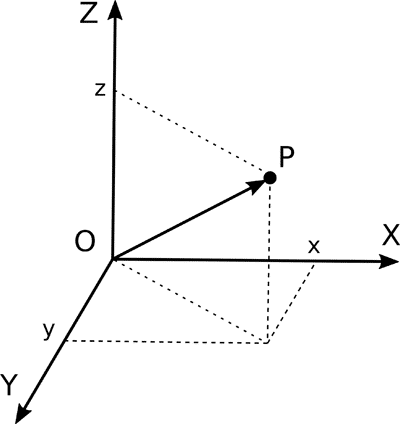
\includegraphics[width=0.3\linewidth]{Immagini/SdR.png}
    \caption{sistema di coordinate cartesiano.}
    \label{fig: SdR}
\end{figure}
Il vettore che unisce i punti $O$ e $P$ si indica con $\vr(t)$, questo permette di calcolare la posizione di $P$ al variare di $t$ sfruttando la scomposizione di $\vr(t)$ lungo gli assi cartesiani
\begin{equation}
    \vr(t)=x(t)\hatu_x+y(t)\hatu_y+z(t)\hatu_z.
\end{equation}
\section{Moto ad una dimensione}
Ci si limita al momento allo studio del moto di corpi puntiformi che si muovono in linea retta.

\begin{defn}[velocità media]
    La velocità media $v_m$ è definita come il rapporto incrementale tra la variazione di posizione e l'intervallo temporale in cui avviene lo spostamento, in formule 
    \begin{equation}
    \label{eq: velocità media}
        v_m=\frac{\Delta x}{\Delta t}=\frac{x_2-x_1}{t_2-t_1}.
    \end{equation}
\end{defn}
Considerando il limite della velocità media $v_m$ si ottiene la velocità istantanea del corpo.
\begin{defn}[velocità istantanea]
    La velocità istantanea $v$ è definita come il limite per $\Delta t\to0$ del rapporto incrementale \eqref{eq: velocità media}, in formule
    \begin{equation}
    \label{eq: velocità istantanea}
        v=\lim_{\Delta t\to0}{\frac{\Delta x}{\Delta t}}=\frac{dx}{dt}.
    \end{equation}
\end{defn}
\begin{obs}
    Considerando l'equazione \eqref{eq: velocità istantanea} e supponendo un moto lungo l'asse $x$, questo avviene nel verso positivo dell'asse se $v>0$ e nel verso negativo se $v<0$.
\end{obs}
A questo punto si è ottenuta una formula della velocità istantanea,
\begin{equation}
    v(t)=\frac{dx}{dt},
\end{equation}
che è a tutti gli effetti un'equazione differenziale risolvibile con il metodo della separazione delle variabili. Quindi si può scrivere
\begin{equation}
    v\,dt=dx.
\end{equation}
Integrando il primo membro tra $t_0$ e $t$ e il secondo tra $x_0$ e $x$ si ottiene
\begin{equation}
    \Delta x=\int_{x_0}^{x}{dx}=\int_{t_0}^{t}{v(t)dt},
\end{equation}
da cui si ricava la legge oraria del moto rettilineo
\begin{equation}\label{eq: legge oraria moto rettilineo}
    x(t)=x_0+\int_{t_0}^{t}{v(t)dt}.
\end{equation}
Analogamente, è possibile definire l'accelerazione media $a_m$.
\begin{defn}[accelerazione media]
    L'accelerazione media $a_m$ è definita come il rapporto incrementale tra la variazione di velocità e l'intervallo temporale in cui avviene questa variazione, in formule 
    \begin{equation}
    \label{eq: accelerazione media}
        a_m=\frac{\Delta v}{\Delta t}=\frac{v(t_2)-v(t_1)}{t_2-t_1}.
    \end{equation}
\end{defn}
Considerando il limite dell'accelerazione media $a_m$ si ottiene l'accelerazione istantanea del corpo.
\begin{defn}[accelerazione istantanea]
    L'accelerazione istantanea $a$ è definita come il limite per $\Delta t\to0$ del rapporto incrementale \eqref{eq: accelerazione media}, in formule
    \begin{equation}
    \label{eq: accelerazione istantanea}
        a=\lim_{\Delta t\to0}{\frac{\Delta v}{\Delta t}}=\frac{dv}{dt}.
    \end{equation}
\end{defn}
\begin{obs}
    Considerando l'equazione \eqref{eq: accelerazione istantanea} e supponendo un moto lungo l'asse $x$, si ha $a>0$ se $v>0$ e $a<0$ se $v<0$.
\end{obs}
A questo punto si è ottenuta una formula dell'accelerazione istantanea,
\begin{equation}
    a(t)=\frac{dv}{dt},
\end{equation}
che è risolvibile nuovamente con il metodo della separazione delle variabili. Quindi si può scrivere
\begin{equation}
    a\,dt=dv.
\end{equation}
Integrando il primo membro tra $t_0$ e $t$ e il secondo tra $v_0$ e $v$ si ottiene
\begin{equation}
    \Delta v=\int_{v_0}^{v(t)}{dv}=\int_{t_0}^{t}{a(t)dt},
\end{equation}
da cui si ricava la formula per la velocità
\begin{equation}
\label{eq: velocità moto rellineo}
    v(t)=v_0+\int_{t_0}^{t}{a(t)dt}.
\end{equation}
Nel caso in cui l'accelerazione $a(t)$ sia una funzione della posizione $a(x)=a(x(t))$ si può scrivere
\begin{equation}
    a=\frac{dv}{dt}=\frac{dv}{dx}\frac{dx}{dt}=v\frac{dv}{dx},
\end{equation}
da cui, usando il metodo di separazione delle variabili, si ottiene
\begin{equation}
    a\,dx=v\,dv.
\end{equation}
Integrando il primo membro tra $x_0$ e $x$ e il secondo tra $v_0$ e $v$ si ottiene
\begin{equation}
    \int_{v_0}^{v}v\,dv=\int_{x_0}^{x}a(x)\,dx,
\end{equation}
da cui
\begin{equation}
\label{eq: v^2 moto rettilineo}
    v^2=v_0^2+2\int_{x_0}^{x}a(x)\,dx.
\end{equation}

\subsection{Moto rettilineo uniforme}
Un corpo si muove di moto rettilineo uniforme (MRU) se si sposta lungo una retta con velocità $v$ costante nel tempo. La legge oraria del MRU si può ricavare dall'equazione \eqref{eq: legge oraria moto rettilineo} considerando appunto $v(t)$ indipendente dal tempo e pertanto ottenendo
\begin{equation}
\label{eq: legge oraria MRU}
    x(t)=x_0+v(t-t_0).
\end{equation}
Ponendo per semplicità $t_0=0$ e $x_0=0$ si ottiene
\begin{equation}
    x(t)=vt.
\end{equation}

\subsection{Moto rettilineo uniformemente accelerato}
Un corpo si muove di moto rettilineo uniformemente accelerato (MRUA) se si sposta lungo una retta con accelerazione $a$ costante nel tempo. La legge oraria del MRUA si può ricavare partendo dall'equazione \eqref{eq: velocità moto rellineo} considerando appunto $a(t)$ indipendente dal tempo e pertanto ottenendo
\begin{equation}\label{eq: v(t) MRU}
    v(t)=v_0+a(t-t_0).
\end{equation}
Si procede ora riconsiderando l'equazione \eqref{eq: legge oraria moto rettilineo} e sostituendo l'equazione \eqref{eq: v(t) MRU} ottenendo
\begin{equation}
    x(t)=x_0+\int_{v_0}^{v}{v_0+a(t-t_0)dt},
\end{equation}
da cui
\begin{equation}\label{legge oraria MRUA}
    x(t)=x_0+v_0(t-t_0)+\frac{1}{2}a(t-t_0)^2.
\end{equation}
Ponendo per semplicità $t_0=0$ e $x_0=0$ si ottiene
\begin{equation}
    x(t)=v_0t+\frac{1}{2}at^2.
\end{equation}
Inoltre, dall'equazione \eqref{eq: v^2 moto rettilineo} si trova
\begin{equation}
    v^2=v_0^2+2a(x-x_0).
\end{equation}

\subsection{Moto armonico semplice}
Un corpo si muove di moto armonico semplice (MAS) se si sposta oscillando con una certa frequenza attorno ad un punto secondo la legge oraria
\begin{equation}
    \label{eq: legge oraria MAS}
    x(t)=A\sin{(\omega t+\phi)},
\end{equation}
dove $\omega$ è la pulsazione e $\phi$ è la fase.
Partendo dall'equazione \eqref{eq: legge oraria MAS} si può ricavare la legge della velocità
\begin{equation}
    \label{eq: v(t) MAS}
    v(t)=\frac{dx(t)}{dt}=\omega A\cos{(\omega t+\phi)}.
\end{equation}
Ponendo $T=t'-t$ e $x(t)=x(t')$ si trova
\begin{equation}
    \omega t'+\phi=\omega t+\phi+2\pi,
\end{equation}
da cui
\begin{equation}
    \omega(t'-t)=\omega T=2\pi,
\end{equation}
dove $T$ è il periodo di oscillazione. Ponendo $t=0$ si trova
\begin{equation}
\label{eq: fase MAS}
    x(0)=A\sin{\phi}\Rightarrow\phi=\arcsin{\left(\frac{x(0)}{A}\right)}.
\end{equation}
Nel caso in cui $\phi=0$ si ha $x(t)=A\sin{\omega t}$, quindi il moto parte dall'origine del sistema di riferimento.

Partendo ora dall'equazione \eqref{eq: v(t) MAS} si può ricavare la legge dell'accelerazione
\begin{equation}
    \label{eq: a(t) MAS}
    a(t)=\frac{dv(t)}{dt}=-A\omega^2\sin{(\omega t+\phi)}=-\omega^2x(t).
\end{equation}
Dall'equazione \eqref{eq: a(t) MAS} si deduce che l'accelerazione è sempre proporzionale allo spostamento, infatti
\begin{equation}
    a(t)=-\omega^2x(t)=\frac{d^2x(t)}{dt^2},
\end{equation}
da cui si ricava l'equazione differenziale di secondo grado del MAS
\begin{equation}
    \label{eq: eq. diff. MAS}
    \frac{d^2x(t)}{dt^2}+\omega^2x(t)=0,\quad x(t)=A\sin{(\omega t+\phi)}.
\end{equation}
Le condizioni al contorno dell'equazione \eqref{eq: eq. diff. MAS} sono per $t=0$
\begin{equation}
    \label{eq: condizioni contorno MAS}
    \begin{cases}
        x_0=A\sin{\phi} \\
        v_0=A\omega\cos{\phi}
    \end{cases}
    \Rightarrow\phi=\arctan{\left(\frac{\omega x_0}{v_0}\right)}.
\end{equation}
Ora dividendo la seconda equazione del sistema \eqref{eq: condizioni contorno MAS} per $\omega$, effettuando il quadrato delle due equazioni e sommandoli si ottiene
\begin{equation}
    A^2=x_0^2+\frac{v_0^2}{\omega^2}.
\end{equation}

\section{Moto in due dimensioni}
La posizione di un corpo in un piano è descritto da un vettore $\vr$ che unisce la posizione del punto all'origine del sistema di riferimento.
\begin{figure}[h]
    \centering
    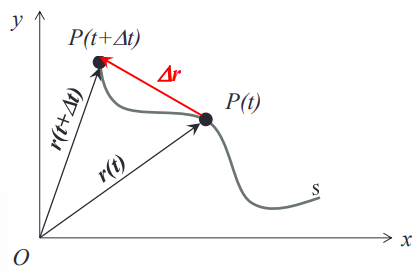
\includegraphics[width=0.5\linewidth]{Immagini/moto in due dimensioni.png}
    \caption{moto in due dimensioni.}
    \label{fig: moto in due dimensioni}
\end{figure}
La velocità istantanea è definita analogamente al caso del moto in una dimensione da
\begin{equation}
\label{eq: velocità moto in due dimensioni}
    \vv=\frac{d\vr}{dt}=\frac{ds}{dt}\hatu_T=v\hatu_T,
\end{equation}
dove $\hatu_T$ è il versore tangente alla traiettoria nel punto $r(t)$. Inoltre, sapendo che $\vr(t)=x(t)\hatu_x+y(t)\hatu_y$, si trova
\begin{equation}
    \vv=\frac{dx}{dt}\hatu_x+\frac{dy}{dt}\hatu_y=v_x\hatu_x+v_y\hatu_y.
\end{equation}
\'E possibile definire la posizione del corpo in coordinate polari, sfruttando l'angolo $\theta(t)$ tra l'asse $x$ e il vettore $\vr(t)$ e il versore radiale $\hatu_r$ parallelo al vettore $\vr(t)$, con cui si può scrivere $\vr(t)=r\hatu_r$. 
\begin{figure}[h]
    \centering
    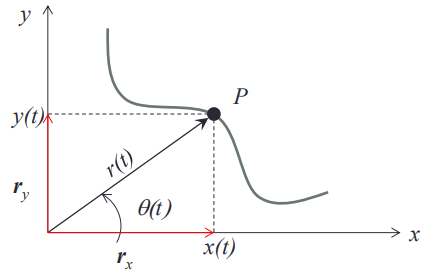
\includegraphics[width=0.55\linewidth]{Immagini/moto in due dimensioni polari.png}
    \caption{moto in due dimensioni in coordinate polari.}
    \label{fig: moto in due dimensioni in coordinate polari}
\end{figure}
La velocità in coordinate polari diventa quindi
\begin{equation}
    \vv=\frac{d\vr}{dt}=\frac{d(r\hatu_r)}{dt}=\frac{d\vr}{dt}\hatu_r+r\frac{d\hatu_r}{dt},\quad\frac{d\hatu_r}{dt}=\frac{d\theta}{dt}\hatu_{\theta}.
\end{equation}
Dunque, la velocità in coordinate polari è data da
\begin{equation}
    \vv=\frac{d\vr}{dt}\hatu_r+r\frac{d\theta}{dt}\hatu_{\theta}=\vv_r+\vv_{\theta},
\end{equation}
dove la prima componente, detta radiale, descrive di quanto si allontana il corpo, mentre la seconda componente, detta trasversa, di quanto esso ruoti.
\begin{figure}[h]
    \centering
    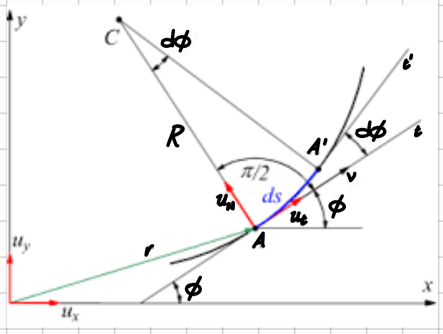
\includegraphics[width=0.6\linewidth]{Immagini/moto 2D diagramma.png}
    \caption{diagramma del moto in due dimensioni in coordinate polari.}
    \label{fig: diagramma del moto in due dimensioni in coordinate polari}
\end{figure}

Conoscendo la legge della velocità si può ricavare la legge dell'accelerazione semplicemente derivando rispetto al tempo l'equazione \eqref{eq: velocità moto in due dimensioni}
\begin{equation}
    \va=\frac{d\vv}{dt}=\frac{d}{dt}(v\hatu_T)=\frac{dv}{dt}\hatu_T+\frac{d\hatu_T}{dt}v,\quad\frac{d\hatu_T}{dt}=\frac{d\varphi}{dt}\hatu_N.
\end{equation}
Dunque, l'accelerazione è data da
\begin{equation}
    \va=\underbrace{\frac{dv}{dt}\hatu_T}_{\substack{\parallel \vv}}+\underbrace{v\frac{d\varphi}{dt}\hatu_N}_{\substack{\perp \vv}}=\va_T+\va_N,
\end{equation}
dove la prima componente esprime la variazione del modulo della velocità, mentre la seconda dipende dalla variazione della direzione di $\vv$, in particolare $\dot{\varphi}$ descrive quanto rapidamente varia la direzione di $\hatu_T$ e quindi di $\hatu_N$. Infine, è possibile riscrivere $\dot{\varphi}$ in funzione di $R$ e $v$. Considerando il differenziale $d\varphi$ si ha
\begin{equation}
    d\varphi=\frac{ds}{R}\Rightarrow\frac{d\varphi}{ds}=\frac{1}{R},
\end{equation}
quindi,
\begin{equation}
    \frac{d\varphi}{dt}=\frac{d\varphi}{ds}\frac{ds}{dt}=\frac{v}{R}.
\end{equation}
Dunque,
\begin{equation}
    \va=\frac{dv}{dt}\hatu_T+\frac{v^2}{R}\hatu_N=\va_T+\va_N.
\end{equation}
\'E possibile distinguere alcuni casi di moto in due dimensioni secondo i valori di $\va_T$ e $\va_N$:
\begin{itemize}
    \item Se $\va_T\neq0$ e $\va_N\neq0$ significa che sta cambiando sia il modulo che la direzione della velocità.
    \item Se $\va_T=0$ e $\va_N\neq0$ significa che il modulo della velocità è costante e varia solo la sua direzione, quindi si ha moto circolare uniforme.
    \item Se $\va_T\neq0$ e $\va_N=0$ significa che la direzione della velocità è costante e varia solo il suo modulo, quindi si ha moto rettilineo vario.
    \item Se $\va_T=0$ e $\va_N=0$ significa che sia il modulo che la direzione della velocità sono costanti, quindi si ha MRU.
\end{itemize}

\subsection{Moto circolare uniforme}
Un corpo si muove di moto circolare uniforme (MCU) se orbita lungo una circonferenza di raggio $R$ a velocità costante. Per studiare questo moto è conveniente usare le coordinate polari
\begin{equation}
    \begin{cases}
        x(t)=R\cos{\theta(t)} \\
        y(t)=R\sin{\theta(t)}
    \end{cases},\quad\theta(t)=\omega t.
\end{equation}
Se il moto non è uniforme allora si hanno
\begin{equation}
    a_T=\frac{dv}{dt},\quad\omega=\frac{v}{R},\quad\alpha=\frac{d\omega}{dt}=\frac{a_T}{R}.
\end{equation}
Dunque, sapendo che $\theta=S/R$ e se $\vv=\vom\times\vr$, si ha
\begin{equation}
    \begin{split}
        \va&=\frac{d\vv}{dt}=\frac{d}{dt}(\vom\times\vr)=\frac{d\vom}{dt}\times\vr+\frac{d\vr}{dt}\times\vom \\
        &=\alpha\times\vr+\vom\times\frac{d\vr}{dt}=\va_T+\va_N.
    \end{split}
\end{equation}
\begin{obs}
    La pulsazione $\omega$ in generale può essere una funzione del tempo anche rispetto alla direzione, in tal caso la legge continua ad essere valida cambiando l'asse di rotazione.
\end{obs}

\subsection{Moto parabolico}
Un corpo si muove di moto parabolico se, partendo con una certa velocità iniziale $v_0$ e un certo angolo $\theta$, percorre una traiettoria sotto l'azione della sola forza di gravità.
\begin{figure}[h]
    \centering
    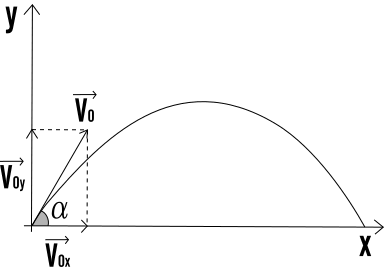
\includegraphics[width=0.4\linewidth]{Immagini/moto parabolico.png}
    \caption{diagramma del moto parabolico.}
    \label{fig: moto parabolico}
\end{figure}
L'accelerazione di gravità è $\va=-g\hatu_y$, la velocità iniziale si scompone lungo gli assi cartesiani come $\vv_0=v_{0x}\hatu_x+v_{0y}\hatu_y$, dove $v_{0x}=v_0\cos{\theta}$ e $v_{0y}=v_0\sin{\theta}$. Quindi, la velocità è data da
\begin{equation}
    \vv=\vv_0+\int_0^t\va(t)\,dt=\vv_0-gt\hatu_y.
\end{equation}
La posizione del corpo è data da
\begin{equation}
    \vr(r)=\vr_0(t)+\int_0^t\vv(t)\,dt=\vv_0t-\frac{1}{2}gt^2\hatu_y=v_{0x}t\hatu_x+(v_{0y}-\frac{1}{2}gt^2)\hatu_y.
\end{equation}
Quindi, le leggi orarie dei moti proiettati sono
\begin{equation}
    \begin{cases}
        x(t)=v_{0x}t \\
        y(t)=v_{0y}t-\dfrac{1}{2}gt^2
    \end{cases}.
\end{equation}
Dalla prima equazione si ricava il tempo $t$ come
\begin{equation}
    t=\frac{x}{v_{0x}}=\frac{x}{v_0\cos{\theta}},
\end{equation}
che sostituito nell'equazione di $y(t)$ restituisce la traiettoria del corpo
\begin{equation}
    y(x)=v_0\sin{\theta}\frac{x}{v_0\cos{\theta}}-\dfrac{1}{2}g\bigg(\frac{x}{v_0\cos{\theta}}\bigg)^2=x\tan{\theta}-\frac{g}{2v_0^2\cos^2{\theta}}x^2.
\end{equation}
\chapter{Dinamica del punto materiale}
La dinamica è la branca della Fisica classica che si occupa di determinare perché un corpo si muove, a differenza della cinematica che descrive unicamente il moto senza occuparsi delle cause che lo hanno generato. L'intera dinamica si basa sui tre principi di Newton.
\begin{axiom}[principi di Newton]\hfill
    \begin{enumerate}
        \item Un corpo non soggetto a forze esterne, o tale che la risultante delle forze esterne agenti su di esso è pari a zero, permane nello stato di quiete o di moto rettilineo uniforme.
        \item La risultante delle forze applicate su un corpo è uguale in modulo al prodotto della massa del corpo per l'accelerazione, ed ha direzione e verso dell'accelerazione.
        \item Quando due corpi interagiscono, la forza che il primo corpo esercita sul secondo è uguale e opposta alla forza che il secondo esercita sul primo.
    \end{enumerate}
\end{axiom}
Secondo tali principi, la forza risultante è data da
\begin{equation}
    \vF=m\va=m\frac{d^2\vr}{dt^2},
\end{equation}
dove $m$ è la massa inerziale che rappresenta la tendenza di un corpo a preservare il proprio stato di quiete o di moto. 
\begin{defn}[sistema di riferimento]
    Un sistema di riferimento inerziale è un sistema che si muove di moto rettilineo uniforme rispetto a un altro e in cui vale il primo principio di Newton.
\end{defn}
\begin{obs}
    Un limite del secondo principio di Newton è che vale per velocità molto inferiori alla velocità della luce. Avvicinandosi a questo limite, gli effetti relativistici sono sempre meno trascurabili. 
\end{obs}
\begin{defn}[forza]
    La forza è la grandezza che esprime e misura l'interazione tra sistemi fisici.
\end{defn}
Nel caso di un moto uniformemente accelerato la risultante delle forze è diversa da zero. In particolare, agisce una forza costante $\vF$ e in generale la componente del moto parallela a $\vF$ è uniformemente accelerata con $\va=\vF/m$. Nelle altre direzioni ortogonali, non c'è moto se le componenti della velocità iniziale lungo tali direzioni sono nulle, oppure si ha un moto rettilineo uniforme se tali velocità sono diverse da zero.

Quando $\vF$ è variabile si ha un moto vario. In particolare, per il moto circolare si ha
\begin{equation}
    \vF=m\vaT+m\vaN=m\frac{dv}{dt}\huT+\frac{mv}{R^2}\huN=\vF_T+\vF_N.
\end{equation}
La risultante delle forze ha una componente ortogonale alla traiettoria $\vF_N$ che fa variare la direzione di $\vv$ e $\vF_T$ ne fa variare il modulo. 
La forza $\vF_N$ non è un tipo diverso di forza, ma è il nome che si dà alla componente ortogonale della risultante. 
\begin{defn}[quantità di moto]
    La quantità di moto (o il momento o l'impulso) di un corpo di massa $m$ che si muove di velocità $\vv$ è definita da 
    \begin{equation}
        \vp=m\vv.
    \end{equation}
\end{defn}
Dalla definizione di quantità di moto è immediato ricavare, se la massa $m$ è costante, che
\begin{equation}
    \vF=\frac{d\vp}{dt}.
\end{equation}
Quindi, l'azione di una forza $\vF$ in un tempo $dt$ produce una variazione $d\vp$ della quantità di moto. 
\begin{teo}[teorema dell'impulso]
    L'impulso di una forza che si esercita su un punto materiale in un intervallo di tempo è uguale alla variazione della quantità di moto del punto in quell'intervallo di tempo. L'impulso $J$ di tale forza è
    \begin{equation}
        J=\int_0^t\vF\,dt=\int_{\vp_0}^{\vp}d\vp=\vp-\vp_0=\Delta\vp.
    \end{equation}
\end{teo}
Da questo teorema si ricava immediatamente che
\begin{equation}
    \vF\Delta t=\Delta\vp.
\end{equation}
Quindi, la variazione dell'impulso $\Delta\vp$ è proporzionale all'intervallo di tempo $\Delta t$ in cui agisce la forza $\vF$. Quando $\vF=0$, allora $\Delta\vp=0$ e l'impulso è costante, ovvero si conserva.
\begin{ex}
    Come primo esempio di applicazione dei principi di Newton, si considerino due corpi di massa $m_1$ e $m_2$ posti a contatto su un piano orizzontale. Su ciascuno dei due corpi agisce una forza peso, $\vN_1=m_1\vg$ e $\vN_2=m_2\vg$ rispettivamente. Si supponga ora di applicare una forza $\vF$ sul corpo di massa $m_1$. Di conseguenza, sul secondo corpo agisce una forza $\vF_{1,2}$ indotta dal primo e, per il terzo principio di Newton, sul primo corpo agisce una forza uguale e opposta $\vF_{2,1}$. Calcolando la risultante delle forze per ciascun corpo si ottengono
\begin{equation}
    \begin{cases}
        F-F_{2,1}=m_1a_1 \\
        F_{1,2}=m_2a_2.
    \end{cases}
\end{equation}
Chiaramente, essendo i corpi a contatto, la loro accelerazione è la stessa, quindi $\va_1=\va_2=\va$. Sommando membro a membro le due equazioni si ottiene
\begin{equation}
    F-F_{1,2}+F_{2,1}=a(m_1+m_2),
\end{equation}
ma dato che $|\vF_{1,2}|=|\vF_{2,1}|$, si ha
\begin{equation}
    F=(m_1+m_2)a\iff\vF=(m_1+m_2)\va.
\end{equation}
\begin{obs}
    Si osservi che le uniche forze che hanno effetto sul moto del sistema sono quelle esterne.
\end{obs}
\end{ex}

\section{Forza d'attrito}
L'attrito è una forza che si oppone al movimento o allo spostamento di un corpo relativo alla superficie su cui si trova: se si manifesta tra superfici in quiete relativa si parla di attrito statico, se invece si manifesta tra superfici in moto relativo si parla di attrito dinamico. Secondo l'interpretazione classica, esistono tre diversi tipi di attrito: radente, volvente e viscoso. 

\subsection{Attrito radente}
L'attrito radente è dovuto allo strisciamento; ad esempio, l'interazione tra due superfici piane che rimangono a contatto mentre scorrono l'una rispetto all'altra. La forza di attrito radente è data da 
\begin{equation}
    \vF_r=\mu_{s,d}\vN,
\end{equation}
dove $\mu_{s}$ è il coefficiente di attrito statico, mentre $\mu_{d}$ è quello di attrito dinamico, e $\vN$ è la forza normale alla superficie di contatto. 

Sperimentalmente, si osserva che il corpo non entra in moto fintanto che la forza applicata non supera $\mu_{s}\vN$. Quando il corpo entra in movimento, comincia ad agire la forza di attrito dinamico $\mu_{d}\vN$ che si oppone a tale moto. Per i coefficienti di attrito radente è sempre verificata la relazione $\mu_{d}<\mu_{s}$.
\begin{ex}
    Si consideri un corpo di massa $m=\SI{3}{\kg}$, coefficiente di attrito dinamico $\mu_{d}=0.04$ e accelerazione $\va=\SI{1.2}{\m/\s^2}$. Le forze agenti sul corpo sono la forza peso $\vF_g=m\vg$, la forza normale $\vN$, la forza di attrito $\vF_{att}=\mu_{d}\vN$ e una forza $\vF$ applicata con un angolo di $\theta$ rispetto all'asse orizzontale. 
    
    Dopo aver scelto un sistema di riferimento con origine coincidente con il centro di massa del corpo, si scompongono le forze lungo gli assi e si scrive la risultante delle forze agenti per ogni asse. In questo modo si ottengono
    \begin{equation}
        \begin{cases}
            \hatu_x:\vN-m\vg+\vF\sin{\theta}=0 \\
            \hatu_y:\vF\cos{\theta}-\mu_{d}\vN=m\va
        \end{cases}.
    \end{equation}
    Dalla prima equazione si ricava
    \begin{equation}
        \vN=m\vg-\vF\sin{\theta},
    \end{equation}
    che sostituita nella seconda restituisce 
    \begin{equation}
        \vF(\theta)=\frac{m(\va+\mu_{d}\vg)}{\cos{\theta}+\mu_{d}\sin{\theta}}.
    \end{equation}
    La forza $\vF(\theta)$ è costante se 
    \begin{equation}
        \frac{d\vF(\theta)}{d\theta}=m(\va+\mu_{d}\vg)\frac{-\sin\theta+\mu_{d}\cos{\theta}}{(\cos{\theta}+\mu_{d}\sin{\theta})^2}=0\iff\tan{\theta}=\mu_{d}.
    \end{equation}
\end{ex}

\subsection{Attrito volvente}
La forza di attrito volvente è una forza resistente che si oppone al moto di rotolamento di un corpo su una superficie. A differenza dell'attrito radente, che agisce tra due superfici che strisciano l'una sull'altra, l'attrito volvente è dovuto alla deformazione del corpo e della superficie di contatto, generando una coppia di forze che tende a rallentare il moto. Per un punto materiale, che idealmente non ha estensione spaziale, l'attrito volvente viene spesso trascurato, poiché dipende da fattori come il raggio e la rigidità del corpo in rotolamento.

\subsection{Attrito viscoso}
La forza di attrito viscoso è una forza dissipativa che agisce su un corpo in movimento all'interno di un fluido, come un liquido o un gas. Essa è proporzionale alla velocità del corpo e dipende dalle proprietà del fluido, come la viscosità, e dalla forma del corpo stesso. Nel caso di un punto materiale, l'attrito viscoso viene modellato come una forza che si oppone al moto e la cui intensità è spesso descritta dalla legge di Stokes per bassi numeri di Reynolds o dalla legge di resistenza quadratica per regimi turbolenti. Questo tipo di attrito è responsabile del rallentamento e dell'eventuale arresto del corpo nel fluido, trasformando parte dell'energia cinetica in calore.

In generale, un corpo immerso in un fluido è soggetto ad una forza di attrito viscoso proporzionale alla velocità $\vv$, ovvero
\begin{equation}
    \vF_v=-b\vv.
\end{equation}
Supponendo che sul corpo agisca verso il basso solamente la forza peso, mentre $\vF_v$ agisce in verso opposto, dal bilancio delle forze si ha
\begin{equation}
    m\vg-b\vv=m\va.
\end{equation}
Scegliendo un sistema di riferimento avente il semiasse $z$ positivo concorde con la forza peso e ponendo $b=Km$, passando ai moduli, si ha l'equazione differenziale
\begin{equation}
    \frac{dv}{dt}=g-Kv.
\end{equation}
Questa si risolve per separazione delle variabili
\begin{equation}
    \begin{split}
        \int_0^v\frac{1}{g-Kv}\,dv&=\int_0^t\,dt \\
        \int_0^v\frac{-K}{g-Kv}\,dv&=-K\int_0^t\,dt \\
        \ln{\bigg|\frac{g-Kv}{g}\bigg|}&=-Kt \\
    \end{split}
\end{equation}
da cui
\begin{equation}
    v(t)=\frac{g}{K}(1-e^{-Kt}).
\end{equation}
La velocità limite è
\begin{equation}
    v_{lim}=\lim_{t\to\infty}v(t)=\frac{g}{K}.
\end{equation}
\begin{obs}
    Allo stesso risultato per la velocità limite ci si può arrivare ponendo $a=dv/dt=0$ dato che il corpo non può accelerare all'infinito.
\end{obs}

\subsection{Piano inclinato}
Si consideri un corpo appoggiato su un piano inclinato ad un angolo $\theta$ rispetto all'orizzontale. Sul corpo agiscono due forze: la forza peso $\vF=m\vg$ e la forza vincolare $\vN$. Scegliendo un sistema di riferimento tale che l'asse $x$ sia parallelo al lato inclinato del piano e l'asse $y$ perpendicolare a tale lato, la forza peso si può scomporre in due componenti $\vF_x=\vF\cos{\theta}=m\vg\cos{\theta}$ e $\vF_y=\vF\sin{\theta}=m\vg\sin{\theta}$. Calcolando la risultante per ogni asse si ottengono
\begin{equation}
    \begin{cases}
        N-mg\cos{\theta}=0 \\
        mg\sin{\theta}=ma
    \end{cases}.
\end{equation}
Dalla seconda equazione si trova immediatamente che
\begin{equation}
    \va=g\sin{\theta}=a\hatu_x.
\end{equation}
Quindi, in assenza di attrito l'accelerazione del corpo non dipende dalla sua massa. Invece, considerando la forza di attrito statico $\vF_{att}=\mu_{s}\vN=-\mu_{s}N\hatu_x$, si hanno
\begin{equation}
    \begin{cases}
        N-mg\cos{\theta}=0 \\
        mg\sin{\theta}-\mu_{s}N=ma
    \end{cases}.
\end{equation}
Dalla prima equazione si ricava $N=mg\cos{\theta}$ che, sostituita nella seconda, restituisce 
\begin{equation}
    a=g(\sin{\theta}-\mu_{d}\cos{\theta}).
\end{equation}
Affinché il moto avvenga, necessariamente la componente lungo l'asse $x$ della forza peso deve superare la forza di attrito statico, ovvero $F_x\ge F_{att}$, da cui si ricava la condizione
\begin{equation}
    \tan{\theta}\le\mu_{s}.
\end{equation}
\begin{figure}[H]
    \centering
    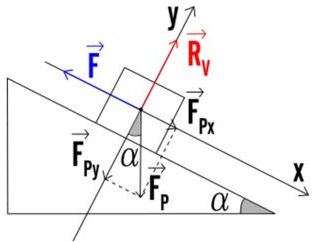
\includegraphics[width=0.4\linewidth]{Immagini/piano inclinato.png}
    \caption{diagramma delle forze di un piano inclinato.}
    \label{fig: piano inclinato}
\end{figure}
Riassumendo, se il corpo è fermo sul piano inclinato esso resta fermo per tutti gli angoli di inclinazione compresi tra zero e $\theta_s$ tale che $\tan{\theta_s}=\mu_{s}$; per $\theta>\theta_s$ il corpo non può restare fermo e scende lungo il piano inclinato. Però, una volta in moto, poiché $\mu_{d}<\mu_{s}$, si può avere moto anche per angoli minori di $\theta_s$, precisamente compresi tra $\theta_s$ e $\theta_d<\theta_s$ tale che $\tan{\theta_d}=\mu_{d}$.

Se invece il corpo all'istante iniziale sta scendendo lungo il piano con velocità $v_0$, esso si ferma se $mg\sin{\theta}<\mu_{d}mg\cos{\theta}$, cioè se $\tan{\theta}<\mu_{d}$, mentre si muove di moto uniformemente accelerato se $\tan{\theta}>\mu_{d}$ e prosegue con velocità $v_0$ se $\tan{\theta}=\mu_{d}$. L'unica differenza rispetto alla partenza da fermo è che si può avere moto anche se $\tan{\theta}<\mu_{d}$ proprio perché c'è una velocità iniziale.

\section{Forza elastica}
La forza elastica (unidimensionale) è una forza di direzione costante con verso rivolto sempre verso la posizione di equilibrio e con modulo proporzionale alla distanza da esso. Pertanto, la forza elastica è data da
\begin{equation}
    \vF_e=-k\vx.
\end{equation}
Dal secondo principio di Newton si ha che l'accelerazione vale
\begin{equation}
    a=-\frac{k}{m}x=-\omega^2x.
\end{equation}
Quindi il moto è armonico semplice con pulsazione $\omega$ e periodo
\begin{equation}
    T=\frac{2\pi}{\omega}=2\pi\sqrt{\frac{m}{k}}.
\end{equation}
Per verificarlo, si parte dal secondo principio di Newton $ma=-kx$ e si riscrive come
\begin{equation}
        \frac{d^2x}{dt^2}+\frac{k}{m}x=0,
\end{equation}
la quale non è altro che l'equazione dell'oscillatore armonico con soluzione
\begin{equation}
    x(t)=A\sin{(\omega t+\phi)}.
\end{equation}
I valori delle costanti $A$ e $\phi$ si ricavano dalle condizioni iniziali
\begin{equation}
    x_0=A\sin{\phi},\quad 0=\omega A\cos{\phi},
\end{equation}
dato che $v(t)=A\omega\cos{(\omega t+\phi)}$. Per $\phi\in(0,2\pi)$ sono possibili due soluzioni: $A=x_0$ per $\phi=\pi/2$ e $A=-x_0$ per $\phi=3\pi/2$; in ogni caso si hanno
\begin{equation}
    x(t)=x_0\cos{(\omega t)},\quad v(t)=-x_0\omega\sin{(\omega t)}.
\end{equation}
Se le condizioni iniziali sono diverse si ottiene sempre un moto armonico con la medesima $\omega$, però il valore dell'ampiezza è in generale diverso da $x_0$. Per esempio, con $x=x_0$ e $v=v_0$ per $t=0$, si ottiene
\begin{equation}
    A=\sqrt{x_0^2+\frac{v_0^2}{\omega^2}},\quad\tan{\phi}=\omega\frac{x_0}{v_0}.
\end{equation}
L'ampiezza $A$ è maggiore di $x_0$ a causa della velocità iniziale diversa da zero. Se in fatti si pone $v_0=0$ si ritrova il risultato precedente. 

\subsection{Tensione dei fili}
Si consideri un elemento infinitesimo $ds$ di un filo teso in quiete. Tale è ``tirato'' dalle due parti restanti di filo e l'equilibrio statico richiede che le due forze agenti sull'elemento di filo siano uguali in modulo e direzione, ma verso opposto.  Questo vale per ogni elemento di filo e il valore della tensione è lo stesso ovunque, altrimenti non ci sarebbe equilibrio. In particolare, ad un estremo $\vT=-\vF$. Per il filo $\overline{AB}$ nel suo insieme deve valere $F_A=F_B=T$: per tendere il filo si applicano le forze $\vF$ e $-\vF$ e la tensione, in modulo, è uguale al modulo di $\vF$. 

Si consideri ora un filo teso in movimento. L'ipotesi che il filo sia inestensibile comporta che tutti i punti del filo, compresi gli estremi, abbiano la stessa accelerazione. Pertanto, due corpi in movimento collegati da un filo teso devono avere la stessa accelerazione. L'ipotesi che il filo abbia massa trascurabile fa sì che il prodotto $ma$ risulti nullo per il filo e per qualsiasi suo elemento, quindi il valore della tensione durante il moto è lo stesso in qualunque punto del filo, come nel caso statico. Lo stesso succede, ovviamente, se il moto è uniforme; in tal caso $a=0$. 

Riassumendo, il filo teso esercita agli estremi la tensione $\vT$, il cui valore dipende dalle forze applicate e che deve essere pensata come la reazione del filo alla forza che lo tende. 

\subsubsection{Due corpi connessi da un filo}
Si considerino due corpi di massa $m_1$ e $m_2$ connessi da un filo di massa $m_f$ posti su un piano orizzontale. Si supponga l'azione di una forza $\vF$ sul corpo di massa $m_2$. 

In questa situazione, studiando il bilancio delle forze per i due corpi e il filo si ottengono
\begin{equation}
    \begin{cases}
        F-T_2=m_2a \\
        T_2-T_1=m_fa \\
        T_1=m_1a
    \end{cases}.
\end{equation}
Quindi, sostituendo la terza equazione nella seconda si ottiene
\begin{equation}
    T_2=(m_1+m_2)a.
\end{equation}
Sostituendo questa nella prima equazione si trova che la forza $F$ vale
\begin{equation}
    F=(m_1+m_2+m_f)a.
\end{equation}
Risolvendo per l'accelerazione e sostituendola nell'espressione delle due tensioni si ottengono
\begin{equation}
    T_1=\frac{m_1}{\sum_im_i},\quad T_2=\frac{m_f+m_1}{\sum_im_i},\quad i=1,2,f.
\end{equation}
\begin{obs}
    Se il filo è ideale, ossia se $m_f=0$, si ha $T_1=T_2$.
\end{obs}

\subsubsection{Pendolo semplice}
Si consideri un pendolo composto da una massa $m$ 
appesa ad un'estremità di un filo ideale di lunghezza $T$. La posizione di equilibrio statico è quella verticale, con la massa ferma e il filo teso. Se si inizia a spostare la massa di un certo angolo $\theta$ rispetto alla verticale, questa comincia ad oscillare intorno alla posizione di equilibrio. Le forze agenti su $m$ sono la forza peso $\vF=m\vg$ e la tensione del filo $\vT$, per cui il moto è regolato da $m\vg+\vT=\va$.
\begin{figure}[h]
    \centering
    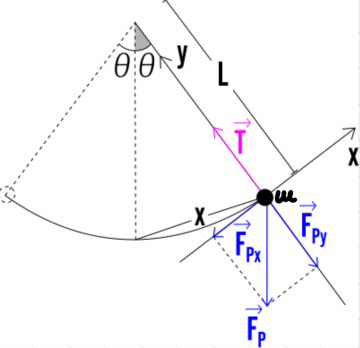
\includegraphics[width=0.4\linewidth]{Immagini/pendolo semplice.png}
    \caption{diagramma delle forze del pendolo semplice.}
    \label{fig: pendolo semplice}
\end{figure}

Scegliendo un sistema di riferimento adeguato, come quello in figura \ref{fig: pendolo semplice}, si può scomporre la forza peso nelle sue componenti
\begin{equation}
    F_x=-mg\sin{\theta},\quad F_y=mg\cos{\theta}.
\end{equation}
\begin{obs}
    Il segno negativo di $F_x$ è dovuto al fatto che la componente tangenziale della forza peso si oppone al moto della massa e tende sempre a riportarla alla posizione di equilibrio. Forze di questo genere sono dette forze di richiamo.
\end{obs}
Quindi, il bilancio delle forze sui due assi è
\begin{equation}
    \begin{cases}
        T-mg\cos{\theta}=ma_c=m\dfrac{v^2}{L} \\
        -mg\sin{\theta}=ma_T
    \end{cases}.
\end{equation}
Dalla seconda equazione si ricava l'equazione differenziale del moto del pendolo
\begin{equation}
    \frac{d^2\theta}{dt^2}+\frac{g}{L}\sin{\theta}=0.
\end{equation}
Tuttavia, per qualunque $\theta$ la soluzione è analiticamente complessa. Per semplificare il problema, si considerano angoli piccoli e si espande il seno in serie di Taylor 
\begin{equation}
    \sin{\theta}=\theta-\frac{\theta}{3!}+\cdots.
\end{equation}
Quantitativamente, per $\theta\le\SI{7}{\degree}$ si può approssimare $\sin{\theta}\simeq\theta$. Quindi, per piccole oscillazioni, l'equazione differenziale si riduce a
\begin{equation}
    \frac{d^2\theta}{dt^2}+\frac{g}{L}\theta=0,
\end{equation}
e coincide con quella del moto armonico semplice, ponendo $\omega^2=g/L$. Dunque, il moto del pendolo è oscillatorio armonico quando l'ampiezza delle oscillazioni è tale da poter approssimare $\sin{\theta}\simeq\theta$. La legge oraria del moto è
\begin{equation}
    \theta(t)=\theta_0\sin{(\omega t+\phi)},
\end{equation}
dove $\theta_0$ è l'ampiezza dell'oscillazione e $\phi$ è la fase iniziale, le quali dipendono dalle condizioni iniziali. Il periodo del moto è
\begin{equation}
    T=2\pi\sqrt{\frac{L}{g}},
\end{equation}
che è indipendente dall'ampiezza (isocronia delle piccole oscillazioni). La legge oraria dello spostamento lungo l'arco di circonferenza $s$ è
\begin{equation}
    s(t)=L\theta(t)=L\theta_0\sin{(\omega t+\phi)}.
\end{equation}
La velocità angolare $\omega(t)$ e la velocità lineare $v(t)$ hanno espressioni
\begin{equation}
    \omega(t)=\frac{d\theta}{dt}=\omega\theta_0\cos{(\omega t+\phi)},\quad v(t)=\frac{ds}{dt}=L\omega\theta_0\cos{(\omega t+\phi)}.
\end{equation}
Note $\theta(t)$ e $v(t)$, si può tornare all'equazione delle forze agenti lungo l'asse $y$ e trovare la tensione del filo
\begin{equation}
    T=m\bigg[g\cos{\theta(t)}+\frac{v^2(t)}{L}\bigg].
\end{equation}

\section{Lavoro, potenza ed energia cinetica}
Si è visto come il secondo principio di Newton si possa esprimere in termini di integrali attraverso il teorema dell'impulso, rivelando che si può calcolare una variazione finita della quantità di moto solo se si è capaci di calcolare l'integrale $\int_{t_0}^{t_1}F(t)\,dt$. Ora si estende il ragionamento considerando la forza come funzione della posizione occupata dal corpo. 

Si consideri un corpo puntiforme $P$ soggetto ad una forza $\vF$ che subisce uno spostamento $\Delta s$. Il lavoro $W$ compiuto dalla forza per lo spostamento $\Delta s$ è definito come il prodotto scalare della forza per lo spostamento, ovvero
\begin{equation}
\label{eq: definizione lavoro}
    W=\vF\cdot\Delta s=F\Delta s\cos{\theta}=F_T\Delta s,
\end{equation}
dove $\theta$ è l'angolo tra $\vF$ e $\Delta s$ e $F_T$ è la proiezione di $\vF$ lungo la direzione dello spostamento. Si possono presentare tre casi:
\begin{enumerate}
    \item Se $\theta<\pi/2$, allora l'accelerazione tangente è concorde con la velocità e la fa aumentare, quindi il lavoro risulta positivo e prende il nome di lavoro motore.
    \item Se  $\theta>\pi/2$, allora l'accelerazione tangente è discorde con la velocità e la fa diminuire, quindi il lavoro risulta positivo e prende il nome di lavoro resistente.
    \item Se $\theta=\pi/2$, allora la forza è ortogonale allo spostamento e il lavoro è nullo, in tal caso la forza è puramente centripeta e non fa variare il modulo della velocità.
\end{enumerate}
Per uno spostamento finito dal punto $A$ al punto $B$ lungo un percorso $C$, il lavoro si ottiene suddividendo tale percorso in una serie di $n$ segmenti $\Delta s_i$ e calcolando per ognuno di essi il lavoro $W_i=\vF_i\cdot\Delta s_i$. Sommando tutti i contributi si ottiene il lavoro totale $W=\sum_iW_i=\sum_i(\vF_i\cdot\Delta s_i)$. Questa è solo un'approssimazione del lavoro reale associato allo spostamento effettivo $C$, ma aumentando il numero di segmenti $n$ questa diventa sempre più accurata. Passando al limite $n\to\infty$, ogni segmento $\Delta s_i$ si confonde con lo spostamento infinitesimo $d\vs$ tangente in ogni punto a $C$, dunque il lavoro totale diventa
\begin{equation}
\label{eq: definizione lavoro spostamento finito}
    W=\int_A^B\vF\cdot d\vs=\int_A^BF\cos{\theta}\,ds.
\end{equation}
In altre parole, il lavoro è l'integrale di linea della forza.

Quando $\vF$ è la somma di $n$ forze $\vF_i$, per ciascuna si può calcolare il corrispondente lavoro e risulta
\begin{equation}
    \begin{split}
        W&=\int_A^B\vF\cdot d\vs=\int_A^B(\vF_1+\cdots+\vF_n)\cdot d\vs \\
        &=\int_A^B\vF_1\cdot d\vs+\cdots+\int_A^B\vF_n\cdot d\vs=W_1+\cdots+W_n.
    \end{split}
\end{equation}
Dunque, il lavoro è pari alla somma dei lavori delle singole forze agenti, ciascuno dei quali può essere positivo, negativo o nullo. 
\begin{defn}[potenza istantanea]
    Si definisce la potenza istantanea $P$ come il lavoro per unità di tempo
    \begin{equation}
        P=\frac{dW}{dt}=\vF\cdot\frac{d\vr}{dt}=\vF\cdot\vv=Fv\cos{\theta}.
    \end{equation}
\end{defn}
In generale, la potenza istantanea è variabile durante il moto e caratterizza la rapidità di erogazione del lavoro. Invece, la potenza media è il rapporto $W/\Delta t$, ossia è il rapporto tra il lavoro totale e l'intervallo di tempo in cui tale lavoro è stato svolto. Questa grandezza è fondamentale per descrivere le prestazioni di una macchina: a parità di lavoro totale svolto, ha maggiore potenza quella che lo eroga nel minor tempo. L'espressione del lavoro può essere scritta in forma infinitesima ottenendo
\begin{equation}
    dW=F_Tds=ma_T\,ds=m\frac{dv}{dt}\,ds=m\frac{ds}{dt}\,dv=mv\,dv.
\end{equation}
Si è trovato il legame esplicito tra il lavoro infinitesimo e la variazione infinitesima del modulo della velocità. Per un percorso finito dal punto $A$ al punto $B$ il lavoro vale
\begin{equation}
    W=\int_A^Bmv\,dv=\frac{1}{2}m(v_B^2-v_A^2)=K_B-K_A=\Delta K,
\end{equation}
dove la quantità $K=mv^2/2$ prende il nome di energia cinetica. Questo è il contenuto del teorema dell'energia cinetica.
\begin{teo}[teorema dell'energia cinetica]
    Qualunque sia la forza che agisce nello spostamento di un corpo puntiforme dal punto $A$ al punto $B$, il lavoro svolto dalla forza è uguale alla variazione dell'energia cinetica del corpo stesso.
\end{teo}

\subsection{Lavoro della forza peso}
Si calcola ora il lavoro della forza peso per uno spostamento generico dal punto $A$ al punto $B$. L'asse $z$ è orientato dal basso verso l'alto ed ha quindi verso opposto alla forza peso. Quindi, da \eqref{eq: definizione lavoro spostamento finito} si ha
\begin{equation}
    W=-mg\int_A^B\hatu_z\cdot d\vs=-mg\int_A^Bdz=-mg(z_B-z_A),
\end{equation}
dato che la forza peso ha come unica componente non nulla quella lungo l'asse $z$ e la componente di $\vr_{AB}$ lungo tale asse è $(z_B-z_A)$. Questo lavoro, dato che dipende unicamente dallo stato iniziale e finale, può essere scritto in termini di una funzione di stato $U(z)$. Dunque,
\begin{equation}
    W=-mg(z_B-z_A)=-[U(z_B)-U(z_A)]=-\Delta U(z)_{AB},
\end{equation}
dove $U(z)$ prende il nome di energia potenziale gravitazionale. 
\newpage
\noindent
Si presentano due casi:
\begin{enumerate}
    \item Se $z_A>z_B$, allora il lavoro svolto è positivo e per far avvenire lo spostamento è sufficiente la sola forza peso.
    \item Se $z_A<z_B$, allora il lavoro svolto è negativo e per fa avvenire lo spostamento è necessaria una forza esterna il cui lavoro superi quello resistente della forza peso oppure che abbia una velocità iniziale tale che la diminuzione di energia cinetica eguagli il lavoro.
\end{enumerate}

\subsection{Lavoro della forza elastica}
Il lavoro della forza elastica (unidimensionale) $\vF=-kx\hatu_x$ per uno spostamento finito lungo l'asse $x$ vale
\begin{equation}
    W=-k\int_A^Bx\hatu_x\cdot d\vs=-k\int_A^Bx\,dx=-\frac{1}{2}k(x_B^2-x_A^2).
\end{equation}
Come per la forza peso, dato che che dipende unicamente dallo stato iniziale e finale, può essere scritto in termini di una funzione di stato $U(x)$. Dunque, 
\begin{equation}
    W=-\frac{1}{2}k(x_B^2-x_A^2)=-[U(x_B)-U(x_A)]=-\Delta U(x)_{AB},
\end{equation}
dove $U(x)$ prende il nome di energia potenziale elastica. I casi che si presentano sono analoghi a quanto detto per la forza peso. 

\subsection{Lavoro della forza d'attrito radente}
Il lavoro della forza di attrito radente $\vF_{att}=-\mu_dN\hatu_s$, dove $\hatu_s$ è parallelo allo spostamento, vale
\begin{equation}
    W=\int_A^B-\mu_dN\hatu_s\cdot d\vs=-\mu_dN\int_A^Bds.
\end{equation}
L'integrale $\int_A^Bds$ non è altro che la lunghezza del percorso da $A$ e $B$ misurata lungo la traiettoria effettiva del corpo puntiforme. Pertanto, per la forza di attrito radente il lavoro dipende dal percorso seguito dal corpo e non è esprimibile in termini di una funzione di stato. Inoltre, il lavoro della forza di attrito è sempre negativo: se cambia il verso del moto, cambia anche quello della forza. Perché il moto possa avvenire o deve agire una forza che produca un lavoro superiore a quello di attrito o il corpo deve possedere una certa energia cinetica iniziale. L'energia cinetica diminuisce lungo il percorso e in $B$ la velocità è minore che in $A$. 

\section{Forze conservative}
Le forze per cui il lavoro non dipende dal percorso prendono il nome di forze conservative. Per il calcolo del lavoro si può considerare qualsiasi percorso che colleghi $A$ e $B$. Il lavoro è pertanto esprimibile in termini dei valori che una funzione di stato agli estremi $A$ e $B$. Questo implica che se si inverte il senso di percorrenza cambia solo il segno del lavoro
\begin{equation}
    \int_A^B\vF\cdot d\vs=-\int_A^B\vF\cdot d\vs.
\end{equation}
Per un percorso chiuso $ABA$ lungo la traiettoria $I$ e $-II$ percorsa in senso inverso si ha
\begin{equation}
    \int_A^B(\vF\cdot d\vs)_I+\int_A^B(\vF\cdot d\vs)_{-II}=\int_A^B(\vF\cdot d\vs)_I-\int_A^B(\vF\cdot d\vs)_{II}=0.
\end{equation}
Dunque, il lavoro svolto da una forza conservativa lungo qualsiasi percorso chiuso è nullo, ovvero
\begin{equation}
    \oint_\gamma\vF\cdot d\vs=0,\quad\forall\gamma.
\end{equation}
Riassumendo:
\begin{enumerate}
    \item per tutte le forze conservative il lavoro esprimere sempre come l'opposto della variazione o dell'energia potenziale relativa alla specifica forza
    \begin{equation}
        W=-\Delta U;
    \end{equation}
    \item non esiste una formula generale dell'energia potenziale, ma l'espressione esplicita dipende dalla particolare forza conservativa associata;
    \item nei casi della forza peso e della forza elastica l'energia potenziale è
    \begin{equation}
        U_p(z)=mgz,\quad U_e(x)=\frac{kx^2}{2}.
    \end{equation}
\end{enumerate}
\begin{obs}
    La relazione $W=\Delta K$ vale per qualsiasi forza agente, non solo per le forze conservative, a differenza di $W=-\Delta U$.
\end{obs}
Se agiscono solo conservative valgono sia $W=-\Delta U$ che $W=\Delta K$, quindi eguagliando le relazioni si ha
\begin{equation}
    U_A+K_A=U_B+K_B,
\end{equation}
ovvero la somma dell'energia cinetica e dell'energia potenziale di un corpo puntiforme che si muove sotto l'azione di forze conservative resta costante durante il moto, ossia si conserva. Tale somma prende il nome di energia meccanica. Pertanto, l'equazione trovata esprime il principio di conservazione dell'energia meccanica 
\begin{axiom}[principio di conservazione dell'energia meccanica]
    In presenza di sole forze conservative, l'energia meccanica di un corpo puntiforme si conserva, ovvero
    \begin{equation}
        E=K+U=costante.
    \end{equation}
\end{axiom}
In generale, quando agiscono sia forze conservative che non conservative, il lavoro complessivo è dato dalla somma del lavoro delle forze conservative $W_C$ e quello delle forze non conservative $W_{NC}$. Quindi, esprimendo $W_C=-\Delta U$, si ha
\begin{equation}
    W_{NC}=\Delta K+\Delta U=(K_B+U_B)-(K_A-U_A)=E_B-E_A=\Delta E.
\end{equation}
Dunque, in presenza di forze non conservative l'energia meccanica non si conserva, bensì la sua variazione è uguale al lavoro svolto dalle forze non conservative. 
\begin{ex}
    Considerando la situazione mostrata in figura \ref{fig: doppio piano inclinato} e, supponendo che $\tan{\theta}>\mu_d$, si vuole determinare la velocità con la quale il corpo arriva al punto $O$. 
    \begin{figure}[h]
        \centering
        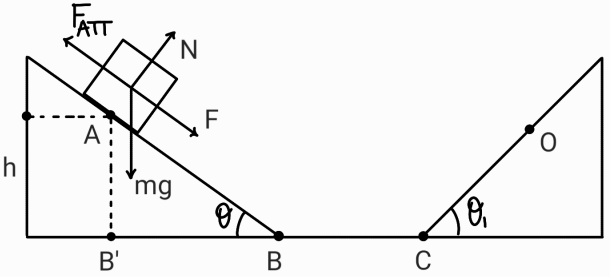
\includegraphics[width=0.57\linewidth]{Immagini/doppio piano inclinato.png}
        \caption{doppio piano inclinato in presenza di attrito.}
        \label{fig: doppio piano inclinato}
    \end{figure}
    
    Il lavoro della forza d'attrito lungo il tratto $\overline{PO}$ è
    \begin{equation}
        W_{att}=-\mu_dN|\overline{PO}|=-\mu_d(mg\cos{\theta})\frac{h}{\sin{\theta}}.
    \end{equation}
    Questo lavoro è uguale alla variazione di energia meccanica, quindi
    \begin{equation}
        -\mu_d(mg\cos{\theta})\frac{h}{\sin{\theta}}=\frac{mv_f^2}{2}-mgh,
    \end{equation}
    da cui si ricava la velocità finale 
    \begin{equation}
        v_f=\sqrt{2gh\bigg(1-\frac{\mu_d}{\tan{\theta}}\bigg)}.
    \end{equation}
\end{ex}
\begin{ex}
    Si consideri il moto di un pendolo semplice che parte dall'angolo di inversione $\theta_0$. Si assuma nulla l'energia potenziale nel punto più basso raggiunto dal pendolo (dove $P$ passa per la verticale). L'altezza di $P$, rispetto al livello zero, è $L(1-\cos{\theta})$. Le energie sono:
    \begin{enumerate}
        \item $U=mgL(1-\cos{\theta_0})$ e $K=0$ nel punto di inversione (il più alto raggiunto);
        \item $U=mgL(1-\cos\theta)$ e $K=mv^2/2$ in punto generico;
        \item $U=0$ e $K=mv_0^2/2$.
    \end{enumerate}
    Dal principio di conservazione dell'energia meccanica si ha
    \begin{equation}
        mgL(1-\cos{\theta})+mv^2/2=mgL(1-\cos{\theta_0}),
    \end{equation}
    da cui si ricava
    \begin{equation}
        v(\theta)=\sqrt{2gL(\cos{\theta}-\cos{\theta_0})}.
    \end{equation}
    In particolare, se $\theta=\pi/2$ si ha $v=\sqrt{2gL}$. Sostituendo $v(\theta)$ a $T-mg\cos{\theta}=mv^2/L$ si ha
    \begin{equation}
        T=mg(3\cos{\theta}-2\cos{\theta_0}),\quad\forall\theta_0.
    \end{equation}
\end{ex}
\begin{obs}
    La relazione integrale $-\Delta U=\int_A^B(F\hatu_x)\cdot d\vx$ può essere resa differenziale in $-dU=Fdx$, da cui si ricava
    \begin{equation}
        F=-\frac{dU}{dx}.
    \end{equation}
    Nel caso tridimensionale si hanno
    \begin{equation}
        F_x=-\frac{\p U}{\p x},\quad F_y=-\frac{\p U}{\p y},\quad F_z=-\frac{\p U}{\p z}.
    \end{equation}
    Usando la nozione di gradiente si ottiene
    \begin{equation}
        \vF=-\nabla U.
    \end{equation}
\end{obs}

\section{Momenti}
\begin{defn}[momento della forza]
    Si definisce il momento della forza come
    \begin{equation}
        \vM=\vr\times\vF.
    \end{equation}
\end{defn}
In generale, per calcolare un momento è necessario definire un polo $O$ rispetto a cui calcolarlo. Quindi, se il momento della forza rispetto al polo $O$ è $\vM=\bm{OP}\times\vF$ e la forza è applicata nel punto $P$, se si cambia polo in $O'$, allora il momento diventa
\begin{equation}
    \vM'=\bm{O'P}\times\vF.
\end{equation}
Dato che $\bm{O'P}=\bm{O'O}+\bm{OP}$, il momento $\vM'$ diventa
\begin{equation}
    \vM'=(\bm{O'O}+\bm{OP})\times\vF=\bm{O'O}\times\vF+\bm{OP}\times\vF=\bm{O'O}\times\vF+\vM.
\end{equation}
Quindi, in generale cambiando polo il momento della forza cambia anch'esso, e $\vM'=\vM$ se $\vF=m\va=0$ o se $\bm{O'O}\parallel\vF$.

Quando ad un punto sono applicate più forze con risultante $\vR=\sum_i\vF_i$, si ha
\begin{equation}
    \vM=\vr\times\vF_1+\cdots+\vr\times\vF_n=\vr\times(\vF_1+\cdots+\vF_n)=\vr\times\vR.
\end{equation}  
Quindi, il momento complessivo è uguale al momento della forza risultante. Pertanto, un sistema di forze applicate nello stesso punto può essere sempre sostituito, nel calcolo dell'accelerazione, del lavoro e del momento complessivo, dalla forza risultante. Questa proprietà non è valida se il punto di applicazione non è lo stesso per ogni forza.
\begin{defn}[momento angolare]
    Si definisce il momento angolare $\vL$ il momento del vettore quantità di moto, ovvero
    \begin{equation}
        \vL=\vr\times\vp=\vr\times m\vv.
    \end{equation}
\end{defn}
Analogamente al caso del momento della forza, se si cambia polo in $O'$, il momento angolare diventa
\begin{equation}
    \vL'=\bm{O'O}\times m\vv+\vL.
\end{equation}
\begin{obs}
    Dalla definizione di momento angolare, usando  $\vv=\vv_r+\vv_\theta$, questo si può riscrivere come
\begin{equation}
    \vL=\vr\times m(\vv_r+\vv_\theta)=m(\vr\times \vv_\theta),
\end{equation}
dove si è usato il fatto che $\vr\parallel\vv_r$ e $\vr\perp\vv_\theta$. Quindi
\begin{equation}
    L=mrv_\theta=mr(r\frac{d\theta}{dt})=mr^2\frac{d\theta}{dt}.
\end{equation}
\end{obs}
Dalla definizione di momento angolare si può ricavare un risultato importante. Derivando tale relazione si ha
\begin{equation}
\label{eq: derivata momento angolare}
    \frac{d\vL}{dt}=\frac{d\vr}{dt}\times m\vv+\vr\times m\frac{d\vv}{dt}.
\end{equation}
Ora si scelga un sistema di riferimento tale per cui il polo $O$ rispetto a cui si calcola il momento angolare sia fermo. Definendo $\vr$ come la distanza tra $O$ e la posizione del corpo puntiforme $P$, questa si può scrivere come $\vr=\vr_P-\vr_O$, dove $\vr_O$ e $\vr_P$  sono la distanza dall'origine del sistema di riferimento, rispettivamente, a $O$ e a $P$. Sostituendo la scomposizione di $\vr$ in \eqref{eq: derivata momento angolare} si ha
\begin{equation}
    \frac{d\vL}{dt}=\frac{d}{dt}(\vr_P-\vr_O)\times m\vv+\vr\times m\frac{d\vv}{dt},
\end{equation}
la quale, dato che $O$ è fermo rispetto al sistema di riferimento scelto, diventa
\begin{equation}
    \frac{d\vL}{dt}=\frac{d\vr_P}{dt}\times m\vv+\vr\times m\frac{d\vv}{dt},
\end{equation}
ma la derivata $d\vr_P/dt$ non è altro che la velocità $v$ del corpo puntiforme in $P$, che è la stessa per ogni sistema di riferimento inerziale, infatti $d\vr_P/dt=d\vr/dt$. Quindi, usando che $\vv\times \vv=0$, si ha
\begin{equation}
    \frac{d\vL}{dt}=\vr\times m\frac{d\vv}{dt}=r\times m\va=\vr\times\vF=\vM.
\end{equation}
Il risultato ottenuto costituisce il teorema del momento angolare.
\begin{teo}[teorema del momento angolare]
    La derivata temporale del momento angolare è uguale al momento della forza se entrambi i momenti sono riferiti allo stesso polo fisso in un sistema di riferimento inerziale, ovvero
    \begin{equation}
    \label{eq: relazione tra momento angolare e momento forze}
        \frac{d\vL}{dt}=\vM.
    \end{equation}
\end{teo}
Il momento della forza può essere nullo sia perché la forza applicata è nulla sia quando $\vr$ e $\vF$ sono paralleli. In questi casi si ha
\begin{equation}
    \frac{d\vL}{dt}=0\Rightarrow L=costante
\end{equation}
Dunque, se il momento delle forze è nullo, il momento angolare di un corpo puntiforme si conserva nel tempo. Integrando l'equazione \eqref{eq: relazione tra momento angolare e momento forze} si ha
\begin{equation}
    \int_0^t\vM\,dt=\Delta\vL.
\end{equation}
Quindi per produrre una variazione finita di momento angolare di un corpo puntiforme è necessaria l'azione, per un certo intervallo di tempo, di una forza. Questa proprietà è analoga al teorema dell'impulso. 
\begin{teo}[teorema del momento dell'impulso]
    Se la forza viene applicata per un intervallo di tempo molto breve, allora $\vr$ è praticamente costante e pertanto 
\begin{equation}
    \vr\times\vJ=\Delta \vL.
\end{equation}
In altre parole, la variazione di momento angolare è uguale al momento dell'impulso applicato.
\end{teo}
\begin{proof}
Dall'integrazione di \eqref{eq: relazione tra momento angolare e momento forze} si ha
    \begin{equation}
        \int_0^t\vM\,dt=\int_0^t\vr\times\vF\,dt=r\times\int_0^t\vF\,dt=\vr\times\vJ,
    \end{equation}
    ma dato che $\int_0^t\vM\,dt=\Delta L$, si trova $\vr\times\vJ=\Delta\vL$
\end{proof}
\begin{obs}
    Facendo riferimento al moto circolare, anche il lavoro può essere espresso in termini del modulo del momento della forza. Infatti
    \begin{equation}
        W=\int_A^B\vF\cdot d\vs=\int_{\theta_A}^{\theta_B}rF_T\,d\theta=\int_{\theta_A}^{\theta_B}M\,d\theta,
    \end{equation}
    dove si è usato il fatto che $ds=r\,d\theta$.
\end{obs}

\section{Forze centrali}
\begin{defn}[forza centrale]
    Una forza centrale è una qualsiasi forza che presenta le seguenti caratteristiche:
    \begin{enumerate}
        \item la direzione della forza deve passare per un punto fisso detto ``centro'';
        \item il modulo della forza deve dipendere esclusivamente dalla distanza dal centro.
    \end{enumerate}
\end{defn}
Un corpo puntiforme soggetto ad una forza centrale $\vF(\vr)$ può compiere una traiettoria qualsiasi, come mostrato in figura \ref{fig: forza centrale}. Per tale corpo, il momento angolare è conservato, infatti
\begin{equation}
    \vM=\vr\times\vF(\vr)=\vr\times(F\hatu_r)=F(\vr\times\hatu_r)=0,
\end{equation}
e pertanto $L=costante$. 
\begin{figure}[H]
    \centering
    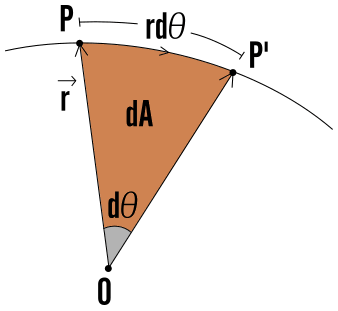
\includegraphics[width=0.4\linewidth]{Immagini/forze centrali.png}
    \caption{corpo puntiforme soggetto ad una forza centrale.}
    \label{fig: forza centrale}
\end{figure}

Quindi, in un intervallo di tempo $dt$, il vettore $\vr$ spazza un'area $dA$ approssimabile ad un triangolo di base $ds=r\,d\theta$ e di altezza $r$ (la differenza tra i lati e l'altezza è trascurabile), ossia
\begin{equation}
    dA=\frac{1}{2}r^2d\theta.
\end{equation}
Derivando rispetto al tempo questa relazione si ha
\begin{equation}
    \frac{dA}{dt}=\frac{1}{2}r^2\frac{d\theta}{dt}=\frac{L}{2m}=costante,
\end{equation}
dove si è usato che $L=mr^2(d\theta/dt)$. Il lavoro di una forza centrale è
\begin{equation}
    W=\int_A^B\vF(\vr)\cdot d\vs=\int_A^BF(r)\hatu_r\cdot d\vs=\int_A^BF(r)\,dr=F(r_B)-F(r_A),
\end{equation}
dove si è usato il fatto che $\hatu_r\cdot d\vs=\cos\theta\,d\vs=d\vr$. Dunque, dato che dipende unicamente dal valore della forza agli estremi, tutte le forze centrali sono conservative. 
\chapter{Moti relativi}
Si consideri un corpo puntiforme $P$ in movimento lungo una generica traiettoria. Il suo moto viene osservato da un sistema di riferimento con centro $O$, che per convezione si chiama fisso, e da un secondo sistema di riferimento con centro $O'$ di coordinate $O'\equiv(x_0,y_0,z_0)$ rispetto ad $O$, che per convezione si chiama mobile. L'origine del sistema mobile ha una velocità $v_{O'}$ rispetto al sistema fisso, inoltre l'insieme dei tre assi in generale ruota rigidamente con velocità angolare $\omega$. L'obiettivo è determinare quali sono le relazioni tra la posizione, la velocità e l'accelerazione del punto $P$, misurate da un osservatore solidale con il sistema fisso, e le corrispondenti grandezze misurate da un osservatore solidale con il sistema mobile. La relazione tra le posizioni del punto $P$, misurate rispetto ai due sistemi di riferimento, è
\begin{equation}
    \vr=\vr_{O'}+\vri,
\end{equation}
dove
\begin{equation}
    \begin{cases}
        \vr=x\hatu_x+y\hatu_y+z\hatu_z \\
        \vr_{O'}=x_0\hatu_x+y_0\hatu_y+z_0\hatu_z \\
        \vri=x'\hatu_{x'}+y'\hatu_{y'}+z'\hatu_{z'} \\
    \end{cases}.
\end{equation}
Quindi, le velocità $\vv$, $\vvi_r$ e $\vv_{O'}$ sono
\begin{equation}
    \begin{split}
        \vv&=\frac{d\vr}{dt}=\frac{d}{dt}(x\hatu_x+y\hatu_y+z\hatu_z) \\
        &=\frac{dx}{dt}\hatu_x+\frac{dy}{dt}\hatu_y+\frac{dz}{dt}\hatu_z+x\frac{d\hatu_x}{dt}+y\frac{d\hatu_y}{dt}+z\frac{d\hatu_z}{dt}\\
        &=\frac{dx}{dt}\hatu_x+\frac{dy}{dt}\hatu_y+\frac{dz}{dt}\hatu_z,
    \end{split}
\end{equation}
\begin{equation}
    \begin{split}
        \vv_{O'}&=\frac{d\vr_O'}{dt}=\frac{d}{dt}(x_0\hatu_x+y_0\hatu_y+z_0\hatu_z) \\
        &=\frac{dx_0}{dt}\hatu_x+\frac{dy_0}{dt}\hatu_y+\frac{dz_0}{dt}\hatu_z+x_0\frac{d\hatu_x}{dt}+y_0\frac{d\hatu_y}{dt}+z_0\frac{d\hatu_z}{dt} \\
        &=\frac{dx_0}{dt}\hatu_x+\frac{dy_0}{dt}\hatu_y+\frac{dz_0}{dt}\hatu_z,
    \end{split}   
\end{equation}
e
\begin{equation}
    \begin{split}
        \vvi_r&=\frac{d\vri}{dt}=\frac{d}{dt}(\xp\hatu_\xp+\yi\hatu_\yi+\zi\hatu_\zi) \\
        &=\frac{d\xp}{dt}\hatu_\xp+\frac{d\yi}{dt}\hatu_\yi+\frac{d\zi}{dt}\hatu_\zi+\xp\frac{d\hatu_\xp}{dt}+\yi\frac{d\hatu_\yi}{dt}+\zi\frac{d\hatu_\zi}{dt},
    \end{split}
\end{equation}
dove si è usato il fatto che $\hatu_x$, $\hatu_y$ e $\hatu_z$ hanno modulo e direzione costante. Usando $\vr=\vr_{O'}+\vri$, la velocità $\vv$ diventa
\begin{equation}
    \begin{split}
        \vv&=\frac{d}{dt}(\vr_{O'}+\vri)=\frac{d\vr_{O}}{dt}+\frac{d\vri}{dt} \\
        &=\frac{dx_0}{dt}\hatu_x+\frac{dy_0}{dt}\hatu_y+\frac{dz_0}{dt}\hatu_z+ \\
        &+\frac{d\xp}{dt}\hatu_\xp+\frac{d\yi}{dt}\hatu_\yi+\frac{d\zi}{dt}\hatu_\zi+\xp\frac{d\hatu_\xp}{dt}+\yi\frac{d\hatu_\yi}{dt}+\zi\frac{d\hatu_\zi}{dt} \\
        &=\vv_{O'}+\vvi+(\xp\vom\times\hatu_\xp+\yi\vom\times\hatu_\yi+\zi\vom\times\hatu_\zi) \\
        &=\vv_{O'}+\vvi+\vom\times(\xp\hatu_\xp+\yi\hatu_\yi+\zi\hatu_\zi) \\
        &=\vv_{O'}+\vvi+\vom\times\vri.
    \end{split}
\end{equation}
La velocità $\vvi$ non è altro che la velocità del punto $P$ rispetto al sistema di riferimento mobile. Dunque, la relazione tra la velocità osservata nel sistema di riferimento fisso $\vv$ e quella osservata nel sistema di riferimento mobile $\vvi$ è data dal teorema delle velocità relative
\begin{equation}
\label{eq: teorema delle velocità relative}
    \vv=\vvi+\vv_{O'}+\vom\times\vri.
\end{equation}
Il termine correttivo $\vv_t=\vv-\vvi=\vv_{O'}+\vom\times\vri$ è detto velocità di trascinamento e dipende dai parametri del sistema di riferimento mobile e dalla posizione del punto $P$ rispetto a tale sistema: corrisponde alla velocità assoluta di un punto solidale con il sistema mobile. Si presentano due casi base:
\begin{enumerate}
    \item Se il sistema mobile non ruota rispetto a quello fisso, ossia $\vom=0$, allora l'equazione \eqref{eq: teorema delle velocità relative} diventa $\vv=\vvi+\vv_{O'}$. In questo caso si parla di moto di trascinamento traslatorio.
    \item Se il sistema mobile non si muove rispetto a quello fisso, ossia $\vv_{O'}$, allora l'equazione \eqref{eq: teorema delle velocità relative} diventa $\vv=\vvi+\vom\times\vri$. In questo caso si parla di moto di trascinamento rotatorio.
\end{enumerate}
Il caso generale può essere pensato come somma di un moto relativo traslatorio e uno rotatorio tra i due sistemi. 

Partendo da $\eqref{eq: teorema delle velocità relative}$ si può ricavare una relazione analoga tra le accelerazioni osservate nei due sistemi di riferimento. Quindi, le accelerazioni $\va$, $\vai_r$ e $\va_{O'}$ sono
\begin{equation}
    \begin{split}
        \va&=\frac{d\vv}{dt}=\frac{d}{dt}\bigg(\frac{dx}{dt}\hatu_x+\frac{dy}{dt}\hatu_y+\frac{dz}{dt}\hatu_z\bigg)=\frac{d^2x}{dt^2}\hatu_x+\frac{d^2y}{dt^2}\hatu_y+\frac{d^2z}{dt^2}\hatu_z,
    \end{split}
\end{equation}
\begin{equation}
    \va_{O'}=\frac{d\vv_{O'}}{dt  }=\frac{d^2x_0}{dt^2}\hatu_x+\frac{d^2y_0}{dt^2}\hatu_y+\frac{d^2z_0}{dt^2}\hatu_z,
\end{equation}
\begin{equation}
    \begin{split}
        \vai_r&=\frac{d\vvi_r}{dt}=\frac{d}{dt}\bigg(\frac{d\xp}{dt}\hatu_\xp+\frac{d\yi}{dt}\hatu_\yi+\frac{d\zi}{dt}\hatu_\zi+\xp\frac{d\hatu_\xp}{dt}+\yi\frac{d\hatu_\yi}{dt}+\zi\frac{d\hatu_\zi}{dt}\bigg) \\
        &=\bigg(\frac{d^2\xp}{dt^2}\hatu_\xp+\frac{d^2\yi}{dt^2}\hatu_\yi+\frac{d^2\zi}{dt^2}\hatu_\zi\bigg)+\frac{d\xp}{dt}\frac{d\hatu_\xp}{dt}+\frac{d\yi}{dt}\frac{d\hatu_\yi}{dt}+\frac{d\zi}{dt}\frac{d\hatu_\zi}{dt}+ \\
        &+\frac{d\xp}{dt}\frac{d\hatu_\xp}{dt}+\frac{d\yi}{dt}\frac{d\hatu_\yi}{dt}+\frac{d\zi}{dt}\frac{d\hatu_\zi}{dt}+\xp\frac{d^2\hatu_\xp}{dt^2}+\yi\frac{d^2\hatu_\yi}{dt^2}+\zi\frac{d^2\hatu_\zi}{dt^2} \\
        &=\va'+2\bigg(\frac{d\xp}{dt}\frac{d\hatu_\xp}{dt}+\frac{d\yi}{dt}\frac{d\hatu_\yi}{dt}+\frac{d\zi}{dt}\frac{d\hatu_\zi}{dt}\bigg)+\xp\frac{d^2\hatu_\xp}{dt^2}+\yi\frac{d^2\hatu_\yi}{dt^2}+\zi\frac{d^2\hatu_\zi}{dt^2} \\
        &=\va'+2\vom\times\bigg(\frac{d\xp}{dt}\hatu_\xp+\frac{d\yi}{dt}\hatu_\yi+\frac{d\zi}{dt}\hatu_\zi\bigg)+\frac{d\vom}{dt}\times(\xp\hatu_\xp+\yi\hatu_\yi+\zi\hatu_\zi) \\
        &+\vom\times[\vom\times(\xp\hatu_\xp+\yi\hatu_\yi+\zi\hatu_\zi)]\\
        &=\va'+2\vom\times\vvi+\frac{d\vom}{dt}\times\vri+\vom\times(\vom\times\vri),
    \end{split}
\end{equation}
dove si è usato che
\begin{equation}
    \begin{split}
        \frac{d^2\hatu_\xp}{dt^2}&=\frac{d}{dt}\bigg(\frac{d\hatu_\xp}{dt}\bigg)=\frac{d}{dt}(\vom\times\hatu_\xp)=\frac{d\vom}{dt}\times\hatu_\xp+\vom\times\frac{d\hatu_\xp}{dt} \\
        &=\frac{d\vom}{dt}\times\hatu_\xp+\vom\times(\omega\times\hatu_\xp),
    \end{split} 
\end{equation}
e così anche per $\hatu_\yi$ e $\hatu_\zi$. Usando $\vr=\vr_{O'}+\vri$, l'accelerazione $\va$ diventa
\begin{equation}
    \begin{split}
        \va&=\frac{d^2\vr_{O'}}{dt^2}+\frac{d^2\vri}{dt^2} \\
        &=\frac{d^2x_0}{dt^2}\hatu_x+\frac{d^2y_0}{dt^2}\hatu_y+\frac{d^2z_0}{dt^2}\hatu_z+\frac{d\vvi}{dt} \\
        &=\va_{O'}+\va'+2\vom\times\vvi+\vom\times(\vom\times\vri)+\frac{d\vom}{dt}\times\vri.
    \end{split}
\end{equation}
L'accelerazione $\vai$ non è altro che l'accelerazione del punto $P$ rispetto al sistema di riferimento mobile. Dunque, la relazione tra l'accelerazione osservata nel sistema di riferimento fisso $\va$ e quella osservata nel sistema di riferimento mobile $\vai$ è data dal teorema delle accelerazioni relative
\begin{equation}
\label{eq: teorema delle accelerazioni relative}
    \va=\va'+\va_{O'}+2\vom\times\vvi+\vom\times(\vom\times\vri)+\frac{d\vom}{dt}\times\vri.
\end{equation}
Il termine correttivo $\va_t=\va_{O'}+2\vom\times\vvi+\vom\times(\vom\times\vri)+(d\vom/dt)\times\vri$ è detto accelerazione di trascinamento e dipende dai parametri del sistema di riferimento mobile e dalla posizione del punto $P$ rispetto a tale sistema. Inoltre, il termine $a_{Cor}=2\vom\times\vvi$ prende il nome di accelerazione complementare o di Coriolis e il termine $\va_{centr}=\vom\times(\vom\times\vri)+(d\vom/dt)\times\vri$ prende il nome di termine centrifugo. Si presentano due casi base:
\begin{enumerate}
    \item Se il sistema mobile non ruota rispetto a quello fisso, ossia $\vom=0$, allora l'equazione \eqref{eq: teorema delle accelerazioni relative} diventa $\va=\vai+\va_{O'}$. In tal caso si parla di moto di trascinamento traslatorio.
    \item Se il sistema di riferimento non accelera rispetto a quello fisso, ossia $\va_{O'}=0$, allora si parla di moto di trascinamento rotatorio e l'equazione \eqref{eq: teorema delle accelerazioni relative} diventa 
    \begin{equation}
        \va=\vai+2\vom\times\vvi+\vom\times(\vom\times\vri)+(d\vom/dt)\times\vri.
    \end{equation}
\end{enumerate}
Il caso generale può essere pensato come somma di un moto relativo traslatorio e uno rotatorio tra i due sistemi. 
\begin{obs}
    Si può presentare anche un altro caso. Se il vettore $\vom$ è costante in modulo, allora $d\vom/dt=0$ e l'equazione \eqref{eq: teorema delle accelerazioni relative} diventa 
    \begin{equation}
        \va=\va'+\va_{O'}+2\vom\times\vvi+\vom\times(\vom\times\vri).
    \end{equation}
\end{obs}

\section{Relatività galileiana}
Si definisce un sistema di riferimento inerziale un sistema in cui valga rigorosamente la legge di inerzia, ossia il primo principio di Newton, in cui un corpo puntiforme non soggetto a forze mantenga il suo stato di quiete o di moto rettilineo uniforme. 

Chiaramente, questa definizione di sistema inerziale ha significato solo se si è in grado di verificare in modo diverso che il corpo non è soggetto a forze. \'E ragionevole supporre che questa interazione si verifichi sia quando il corpo è sufficientemente lontano da qualsiasi altro in modo da poter trascurare ogni interazione, sia quando è possibile bilanciare le forze agenti in modo che la risultante sia nulla. Si supponga di trovarsi in uno di questi casi e di poter verificare se il sistema di riferimento in cui si osserva il moto è inerziale o meno. 

In un sistema di riferimento inerziale il secondo principio di Newton ha l'espressione più semplice: le forze a primo membro sono le ``forze vere'' ovvero quelle che derivano dalle interazioni fondamentali, e la risultante è proporzionale all'accelerazione misurata in quel sistema di riferimento.

Si consideri ora un altro sistema di riferimento che si muove di moto traslatorio rettilineo uniforme rispetto ad un certo sistema di riferimento inerziale. In tal caso si ha $v_{O'}=costante$, $\va_{O'}=0$ e $\vom=0$. Da \eqref{eq: teorema delle accelerazioni relative} si ricava immediatamente che $\va=\vai$: le accelerazioni di un corpo puntiforme misurate nei due sistemi di riferimento sono uguali. Se $\va=0$, allora anche $\vai=0$ e pure il secondo sistema di riferimento è inerziale. 

Dunque, definito un sistema di riferimento inerziale, tutti gli altri sistemi di riferimento in moto rettilineo uniforme rispetto a questo sono anch'essi inerziali. Per tali sistemi il secondo principio di Newton ha la stessa forma, cioè se in $O$ si misura $\va$, e quindi la forza agente è $\vF=m\va$, allora in $O'$ si misura sempre $\va$, e quindi la forza è sempre $\vF=m\va$. Una conseguenza importante è che, essendo la dinamica la stessa, non è possibile stabilire, tramite misure effettuate in questi diversi sistemi di riferimento, se uno di essi è in quiete o in moto. Non ha senso quindi il concetto di moto assoluto. Questi concetti sono alla base della relatività galileiana. 

Se il moto del secondo sistema è accelerato rispetto al sistema inerziale, ovvero sia perché $\vai\neq0$ oppure $\vom\ne0$ o per entrambe le ragioni, si osserva che il secondo principio di Newton non è proporzionale all'accelerazione del punto, misurata nel sistema accelerato. Infatti, se si moltiplica \eqref{eq: teorema delle accelerazioni relative} per la massa $m$ del corpo, e si ricorda che $\vF=m\va$, si ottiene 
\begin{equation}
\label{eq: forza in un SdRNI}
    \vF'=m\vai=\vF-m\va_t-m\va_{Cor}.
\end{equation}
Quindi, in un sistema di riferimento non inerziale il prodotto della massa del corpo puntiforme per l'accelerazione misurata in quel sistema è uguale alla forza vera agente sul punto più le forze apparenti. Queste ultime, essendo sempre proporzionali alla massa del corpo e pertanto vengono anche chiamate forze di inerzia, appaiono solo nel sistema non inerziale, dove costituiscono il termine correttivo che permette di tornare all'espressione $\vF'=m\vai$. Le forze apparenti non derivano dalle interazioni fondamentali e non esistono in un sistema di riferimento inerziale. Da questo risulta chiara l'importanza di riferire le misure ad un sistema di riferimento inerziale. In tale sistema infatti la descrizione di un fenomeno dinamico è più semplice e più aderente a quelli che si suppone siano i meccanismi di base. Ad esempio, se si osserva in un sistema inerziale un corpo puntiforme che descrive una traiettoria curva, allora si può affermare che su di esso agisce una forza vera, mentre se $\vF=0$, allora il moto è rettilineo, e viceversa. Invece, se in un sistema non inerziale si osserva che $\vF=0$, da \eqref{eq: forza in un SdRNI} si vede come ciò non comporti $\vai=0$ e quindi l'osservazione di un moto rettilineo uniforme. Analogamente, una traiettoria curva non implica la presenza di una forza vera, ma potrebbe essere l'effetto di una forza apparente. 

Tutto ciò non significa che la descrizione del moto in un sistema inerziale sia corretta, mentre quella in un sistema non inerziale sia errata. In entrambi i sistemi, note le condizioni iniziali e le forze agenti, le previsioni tramite $\vF=m\va$ e \eqref{eq: forza in un SdRNI} sono corrette, ma la descrizione non inerziale è più complessa. 

\section{Moto di trascinamento traslatorio}
Si consideri la situazione in figura \ref{fig: MTTR}. Si presentano due possibilità: 
\begin{enumerate}
    \item Il moto di $O'$ è uniforme, ossia $\va_{O'}=0$, e quindi anche $O'$ è inerziale.
    \item Il moto di $O'$ non è uniforme, ossia $\va_{O'}\neq0$, e quindi $O'$ non è inerziale.
\end{enumerate}
\begin{figure}[H]
    \centering
    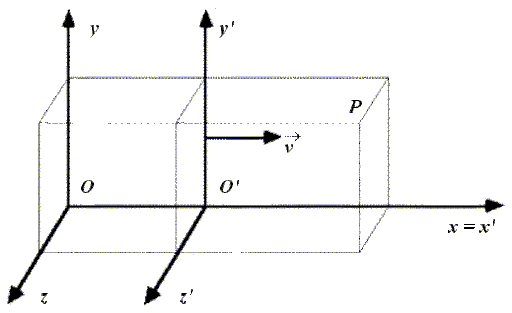
\includegraphics[width=0.45\linewidth]{Immagini/MTTR.png}
    \caption{un sistema fisso $O$ e un sistema mobile $O'$ in moto di trascinamento traslatorio rettilineo lungo l'asse $x$.}
    \label{fig: MTTR}
\end{figure}
Nel primo caso, le relazioni per la velocità e l'accelerazione sono 
\begin{equation}
    \vv=\vvi+\vv_{O'},\quad\va=\vai,
\end{equation}
mentre il legame tra i raggi vettori è 
\begin{equation}
    \vr=\vr_{O'}+\vri=\vv_{O'}t+\vri,
\end{equation}
infatti $\vr_{O'}=\vv_{O'}t$ nell'ulteriore ipotesi che per $t=0$ le origini coincidano. Le relazioni vettoriali possono essere proiettate sugli assi cartesiani fornendo le relazioni tra le componenti dei vettori. Le relazioni che si ottengono prendono il nome di trasformazione galileiane e sono
\begin{equation}
\label{eq: trasformazioni di Galileo}
    \begin{cases}
        x'=x-v_{O'}t \\
        v_x'=v_x-v_{O'} \\
        a_x'=a_x
    \end{cases},\quad
    \begin{cases}
        y'=y \\
        v_y'=v_y \\
        a_y'=a_y
    \end{cases},\quad
    \begin{cases}
        z'=z \\
        v_z'=v_z \\
        a_z'=z_z
    \end{cases}.
\end{equation}
Nel secondo caso, supponendo che $O'$ abbia un'accelerazione costante $\va_{O'}=\va_t$ e una velocità iniziale $\vv_{i}$, ambedue parallele e concordi all'asse $x\equiv x'$. Quindi, la posizione e la velocità $O'$ sono espresse da
\begin{equation}
    x_{O'}=v_it+\frac{1}{2}a_tt^2,\quad v_{O'}=v_i+a_tt,
\end{equation}
e le relazioni per la velocità e l'accelerazione sono
\begin{equation}
    \vv=\vvi+\vv_{O'},\quad\va=\vai+\va_{O'}.
\end{equation}
Dunque, le relazioni \eqref{eq: trasformazioni di Galileo} diventano
\begin{equation}
    \begin{cases}
        x'=x-v_it-\dfrac{1}{2}a_tt^2 \\
        v_x'=v_x-v_i-a_tt \\
        a_x'=a_x-a_t
    \end{cases},\quad
    \begin{cases}
        y'=y \\
        v_y'=v_y \\
        a_y'=a_y
    \end{cases},\quad
    \begin{cases}
        z'=z \\
        v_z'=v_z \\
        a_z'=z_z
    \end{cases}.
\end{equation}

\section{Moto di trascinamento rotatorio uniforme}
Si consideri la situazione mostrata in figura \ref{fig: MTRU}. In questo caso si ha che $\vr=\vri$ (origini coincidenti), $\vv_{O'}=0$, $\va_{O'}=0$, $\vom=costante$ e le relazioni per la velocità e l'accelerazione sono
\begin{equation}
    \vv=\vvi+\vom\times\vr,\quad\va=\vai+\vom\times(\vom\times\vr)+2\vom\times\vvi.
\end{equation}
Quindi, l'equazione \eqref{eq: forza in un SdRNI} diventa
\begin{equation}
    \vF+\vF_{centr}+\vF_{Cor}=m\vai,
\end{equation}
dove $\vF_{centr}=-m\vom\times(\vom\times\vr)$ è la forza centrifuga e $\vF_{Cor}=-2\vom\times\vvi$ è la forza di Coriolis, le quali hanno lo stesso ruolo della forza $-m\va_t$ visto in precedenza.  
\begin{figure}[h]
    \centering
    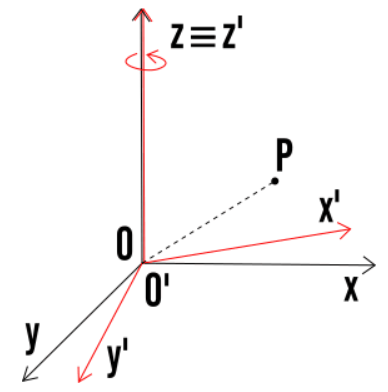
\includegraphics[width=0.3\linewidth]{Immagini/MTRU.png}
    \caption{un sistema fisso $O$ e un sistema mobile $O'$ in moto di trascinamento rotatorio uniforme.}
    \label{fig: MTRU}
\end{figure}
\begin{ex}
    Si consideri un filo a piombo su una piattaforma orizzontale ruotante attorno ad un asse con il punto di sospensione fuori dall'asse di rotazione. Il filo si inclina di un angolo $\theta$ rispetto alla verticale crescente con $\vom$ e con la distanza $r$ dall'asse di rotazione. Il corpo puntiforme non si muove rispetto alla piattaforma, quindi $\vvi=0$ e $\vF_{Cor}=0$.
    \begin{figure}[H]
        \centering
        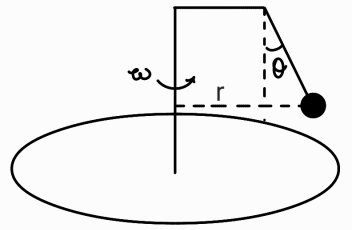
\includegraphics[width=0.37\linewidth]{Immagini/pendolo relativo.png}
        \caption{filo a piombo ruotante.}
        \label{fig: filo a piombo ruotante}
    \end{figure}
    
    Per un osservatore inerziale, il moto di rotazione del corpo è determinato dalle forze vere, ovvero dalla forza peso $m\vg$ e dalla tensione del filo $\vT$. Quindi
    \begin{equation}
        \vT+m\vg=m\va=m\omega^2r\hatu_r.
    \end{equation}
    Dalla figura \ref{fig: filo a piombo ruotante}, si hanno
    \begin{equation}
        T\sin{\theta}=m\omega^2r,\quad T\cos{\theta}=mg,\quad \tan{\theta}=\frac{a}{g}=\frac{\omega^2r}{g}.
    \end{equation}
    La forza centripeta richiesta per mantenere in rotazione il corpo su una circonferenza di raggio $r$ è fornita dalla componente orizzontale della tensione. 
    
    Invece, per un osservatore solidale alla piattaforma il corpo puntiforme è fermo, per cui 
    \begin{equation}
        \vT+m\vg+\vF_{centr}=0\Rightarrow\vF_{centr}=m\omega^2r\hatu_r.
    \end{equation}
    Le forze sono equilibrate dalla forza centrifuga apparente. In ogni caso, misurato $\theta$ è possibile calcolare l'accelerazione centrifuga, ovvero l'accelerazione con cui ruota il sistema non inerziale, usando $\tan{\theta}=\omega^2r/g$.
\end{ex}
\chapter{Dinamica dei sistemi di punti materiali}
Si consideri un sistema di $n$ punti materiali, con $n>1$, interagenti tra di loto e con il resto dell'Universo. La forza $\vF_i$ agente sull'i-esimo punto è la somma delle forze interne degli altri $n-1$ punti e delle forze esterne agenti sul punto, quindi
\begin{equation}
    \vF_i=m_i\va_i=\vF_i^{int}+\vF_i^{ext}.
\end{equation}
Questa scomposizione è molto utile, ma dal moto del punto $P$ non è possibile evidenziare i due tipi di forze, in quanto il suo moto è determinato dalla risultante $\vF_i$. La distinzione tra forze interne ed esterne dipende da come viene definito il sistema di punti. Alle forze interne si applica il terzo principio di Newton: se il punto i-esimo esercita sul punto j-esimo una forza $\vF_{i,j}$, allora il punto j-esimo esercita una forza $\vF_{j,i}$ sul punto i-esimo, e tali forze hanno la stessa retta d'azione, stesso modulo, ma verso opposto e possono essere attrattive o repulsive. La somma delle forze che agiscono su tutti i punti del sistema è data da
\begin{equation}
    \nsum_i\vF_i=\nsum_i\vF_i^{int}+\nsum_i\vF_i^{ext}.
\end{equation}
Tuttavia, anche se in generale la risultante $\vF_i^{int}$ delle forze interne agenti  sull'i-esimo punto è diversa da zero, la risultante di tutte le forze interne del sistema è nulla perché, in base al terzo principio di Newton, esse sono a due uguali ed opposte. Quindi, la somma delle forze agenti su tutti i punti del sistema è data da
\begin{equation}
    \nsum_i\vF_i=\nsum_i\vF_i^{ext}.
\end{equation}
\begin{obs}
    Si osservi che il terzo principio di Newton si applica a qualsiasi interazione, anche alle forze esterne. In tal caso, la reazione si applica al resto dell'Universo e non al sistema, di cui si vuole studiare il moto. 
\end{obs}
Per ciascun punto $P_i$ di massa $m_i$ sottoposto alla forza $\vF_i$ si possono definire: la posizione $\vr_i$, la velocità $\vv_i$, l'accelerazione $\va_i$, la quantità di moto $\vp_i=m\vv_i$, il momento angolare $\vL_i=\vr_i\times m\vv_i$ e l'energia cinetica $K_i=m_i\vv_i^{\,2}/2$.

Per il sistema complessivo si possono definire: la quantità di moto totale $\vp=\nsum_i\vp_i=\sum_im_i\vv_i$, il momento angolare totale $\vL=\sum_i\vL_i=\sum_i\vr_i\times m_i\vv_i$ e l'energia cinetica totale $K=\sum_iK_i=\sum_im_i\vv_i^{\,2}/2$.

\section{Centro di massa}
\begin{defn}[centro di massa]
    Si definisce il centro di massa di un sistema di punti materiali il punto geometrico la cui posizione è individuata, nel sistema di riferimento considerato, dal raggio vettore
    \begin{equation}
        \vr_{CM}=\frac{\sum_im_i\vr_i}{\sum_im_i}=\frac{m_1\vr_1+\cdots+m_n\vr_n}{m_1+\cdots+m_n}.
    \end{equation}
\end{defn}
Le componenti di $\rcm$, ovvero le coordinate del centro di massa in un sistema di coordinate cartesiane con origine $O$, sono
\begin{equation}
    \xcm=\frac{\sum_im_ix_i}{\sum_im_i},\quad\ycm=\frac{\sum_im_iy_i}{\sum_im_i},\quad\zcm=\frac{\sum_im_iz_i}{\sum_im_i}.
\end{equation}
Da queste definizioni, si vede che la ``posizione'' del centro di massa non dipende dal sistema di riferimento, mentre le sue coordinate variano a seconda del sistema prescelto. Se si considera un secondo sistema di riferimento $O'$, le posizioni dei punti $P_i$ sono individuate rispettivamente dai raggi $\vr_i$ e $\vri_i$ con
\begin{equation}
    \vr_i=\vri_i+\vr_{O'}.
\end{equation}
La posizione del centro di massa rispetto ad $O'$ quindi è
\begin{equation}
    \vricm=\frac{\sum_im_i\vri_i}{\sum_im_i}=\frac{\sum_im_i(\vr_i-\vr_{O'})}{\sum_im_i}=\frac{\sum_im_i\vr_i}{\sum_im_i}-\vr_{O'}=\rcm-\vr_{O'}.
\end{equation}
Se gli $n$ punti sono in movimento, la posizione del centro di massa varia. In base a tale definizione, la velocità del centro di massa è
\begin{equation}
    \vcm=\frac{d\rcm}{dt}=\frac{\sum_im_i\dfrac{d\vr_i}{dt}}{\sum_im_i}=\frac{\sum_im_i\vv_i}{\sum_im_i}=\frac{\vp}{m},
\end{equation}
dove $m=\sum_im_i$ è la massa totale del sistema di punti materiali. Dunque, la quantità di moto di un sistema di punti materiali è uguale alla quantità di moto $m\vcm$ del centro di massa, considerato come un punto materiale che abbia  posizione $\rcm$, velocità $\vcm$ e massa pari alla massa totale $m$ del sistema. Analogamente, l'accelerazione del centro di massa è
\begin{equation}
    \acm=\frac{d\vcm}{dt}=\frac{\sum_im_i\dfrac{d\vv_i}{dt}}{\sum_im_i}=\frac{\sum_im_i\va_i}{\sum_im_i}=\frac{\sum_im_i\va_i}{m}.
\end{equation}
Se il sistema di riferimento è inerziale, allora 
\begin{equation}
    m_i\va_i=\vF_i=\vF_i^{int}+\vF_i^{ext},
\end{equation}
che sostituita nell'espressione di $\acm$, moltiplicandola per $m$, restituisce
\begin{equation}
    m\acm=\sum_im_i\va_i=\sum_i(\vF_i^{int}+\vF_i^{ext})=\sum_i\vF_i^{ext}=\vR^{ext},
\end{equation}
dato che la risultante delle forze interne è nulla. Si arriva al seguente teorema.
\begin{teo}[teorema del centro di massa]
    Il centro di massa si muove come un punto materiale in cui sia concentrata tutta la massa del sistema e a cui sia applicata la risultante delle forze esterne, ovvero
    \begin{equation}
    \label{eq: teorema del centro di massa}
        \vR^{ext}=m\acm.
    \end{equation}
\end{teo}
Da \eqref{eq: teorema del centro di massa} si ricava anche che
\begin{equation}
    \vR^{ext}=m\acm=m\frac{d\vcm}{dt}=\frac{d(m\vcm)}{dt}=\frac{d\vp}{dt},
\end{equation}
ovvero che la risultante delle forze esterne è uguale alla derivata temporale della quantità di moto totale del sistema. 

Dunque, il moto del centro di massa è determinato unicamente dalle forze esterne. L'accelerazione delle forze interne non può modificare la stato di moto del centro di massa; invece il moto di ciascun punto dipende dall'azione delle forze esterne ed interne agenti su di esso.

La definizione introdotta di centro di massa è matematica, nel senso che non esiste il punto materiale centro di massa, ma quest'ultima è distribuita nei singoli punti che si muovono sotto l'azione delle forze esterne ed interne. Tuttavia, questo punto matematico gode di notevoli proprietà. Facendo riferimento a $\vp$ e $\vR^{ext}$, si può dire che il centro di massa rappresenta il moto globale o di insieme dei punti materiali. Il fatto che ad un certo istante $\vcm$ abbia un determinato valore significa solamente che il sistema in media si sta spostando in quella data direzione, anche se nessuna delle singole $\vv_i$ coincide con $\vcm$. Analogamente, il fatto che $\acm$ abbia un certo valore a causa dell'azione di $\vR^{ext}$ indica che in media il sistema sta accelerando in quella data direzione. In effetti, $\rcm$, $\vcm$ e $\acm$ sono le medie pesate sulle masse dei raggi vettori, velocità e accelerazioni dei singoli punti e pertanto forniscono informazioni di proprietà medie e non sul moto dei singoli punti. 
\begin{obs}
    Si osservi che le relazioni $\vR^{ext}=m\acm$ e $\vp=m\vcm$ del centro di massa coincidono con quelle del punto materiale ideale, di cui il centro di massa è l'esempio migliore, senza approssimazioni sulle dimensioni o sul tipo di moto.
\end{obs}

\section{Conservazione della quantità di moto}
Se il sistema di punti è isolato, ossia non è soggetto a forze esterne, oppure l'azione di queste forze è tale che la loto risultante sia nulla, si hanno
\begin{equation}
\label{eq: conervazione della quantità di moto}
    \acm=0,\quad\vcm=costante,\quad\vp=costante.
\end{equation}
Questo risultato esprime il seguente teorema.
\begin{teo}[principio della conservazione della quantità di moto]
    Quando la risultante della forze esterne è nulla, la quantità di moto totale del sistema rimane costante nel tempo e il centro di massa si muove di moto rettilineo uniforme o resta in quiete. 
\end{teo}
L'equazione $\vp=costante$ è una legge vettoriale e si può scomporre in tre relazioni valide per i moti proiettati sugli assi, $p_x=costante$, $p_y=costante$ e $p_z=costante$. Anche se $\Rext=0$, le quantità di moto dei vari punti $m_i\vv_i$ in generale variano nel tempo, mentre resta costante solo la loro somma $\sum_im_i\vv_i$.
\begin{obs}
    La conservazione della quantità di moto può avvenire anche solo per una o due delle componenti di $\vp$. 
\end{obs}
Si considerino ora due punti isolati che possono interagire solo tra loro, in questo caso
\begin{equation}
    \vp=\vp_1+\vp_2=m_1\vv_1+m_2\vv_2.
\end{equation}
Derivando $\vp$ rispetto al tempo si ha
\begin{equation}
    \frac{d\vp}{dt}=\frac{d}{dt}(m_1\vv_1+m\vv_2)=m_1\va_1+m_2\va_2=\vF_1+\vF_2=0\Rightarrow \vF_1=-\vF_2.
\end{equation}
Dunque, il principio di conservazione della quantità di moto per un sistema isolato di due punti ha come conseguenza che le forze tra i due punti sono uguali in modulo ma opposte in verso. Questo risultato non è completamente equivalente al terzo principio di Newton in quanto $\vF_1=-\vF_2$ non implica che le due forze agiscano sulla stessa retta d'azione. Con questa osservazione, si può dire che c'è un'equivalenza tra il principio di conservazione della quantità di moto e il terzo principio di Newton, generalizzabile a sistemi più complessi. 
\begin{obs}
    In realtà il principio di conservazione della quantità di moto per un sistema isolato è di portata più generale: si dimostra che questo discende dall'omogeneità dello spazio, ossia dal fatto che non esiste un'origine privilegiata per i sistemi di riferimento. 
\end{obs}
Il principio di conservazione della quantità di moto permette anche di definire dinamicamente la massa, indipendentemente dalla forza peso. Si considerino due punti materiali fermi agli estremi di una molla compressa. Dato che il centro di massa è in quiete, la quantità di moto del sistema dei due punti è nulla, $\vp=0$. Lasciando espandere la molla, i due punti si muovono in versi opposti e dato che agiscono durante il moto solo forze interne, continua a valere $\vp=0$. Pertanto, si ha
\begin{equation}
    \vp=m_1\vv_1+m_2\vv_2=0\Rightarrow m_2=m_1\frac{\vv_1}{\vv_2}.
\end{equation}
Dunque, è possibile misurare il valore di una qualsiasi massa, rispetto ad un campione, tramite misure di velocità. 

\section{Conservazione del momento angolare}
Si consideri il momento angolare totale di un sistema di punti materiali rispetto ad un polo $O$. Detto $\vr_i$ il raggio vettore $\overline{OP_i}$ si ha
\begin{equation}
    \vL=\nsum_i\vr_i\times m\vv_i.
\end{equation}
In generale, il polo $O$ può non coincidere con l'origine del sistema di riferimento e può non essere fisso, quindi $\vr_i$ può avere entrambi gli estremi in movimento, con velocità $\vv_i$ e $\vv_O$ nel sistema di riferimento inerziale da cui si osserva il sistema di punti. Derivando $\vL$ rispetto al tempo si ottiene
\begin{equation}
    \frac{d\vL}{dt}=\nsum_i\frac{d\vr_i}{dt}\times m_i\vv_i+\nsum_i\vr_i\times m_i\frac{\vv_i}{dt}.
\end{equation}
Dato che $\vr_i$ restituisce la posizione di $P_i$ rispetto ad $O$ ed entrambi possono essere in movimento, si ha
\begin{equation}
    \frac{d\vr_i}{dt}=\vv_i-\vv_O.
\end{equation}
Inoltre, essendo il sistema inerziale si ha 
\begin{equation}
    m_i\frac{d\vv_i}{dt}=m_i\va_i=\vF_i^{int}+\vF_i^{ext}.
\end{equation}
Ne segue che
\begin{equation}
    \begin{split}
        \frac{d\vL}{dt}&=\nsum_i(\vv_i-\vv_O)\times m_i\vv_i+\nsum_i\vr_i\times(\vF_i^{int}+\vF_i^{ext}) \\
        &=\nsum_i\vv_i\times m_i\vv_i-\nsum_i\vv_O\times m_i\vv_i+\nsum_i\vr_i\times\vF_i^{int}+\nsum_i\vr_i\times\vF_i^{ext} \\
        &=-\vv_O\times\vcm+\vM^{int}+\vM^{ext}.
    \end{split}
\end{equation}
Il vettore $\vM^{int}=\nsum_i\vr_i\times\vF_i^{int}$ è il momento delle forze interne, mentre $\vM^{ext}=\nsum_i\vr_i\times\vF_i^{ext}$ è il momento delle forze esterne, entrambi rispetto al polo $O$. 

Si dimostra ora che $\vM^{int}=0$. Considerando due punti $P_i$ e $P_j$, la somma dei momenti delle due forze interne $\vF_{i,j}$ e $\vF_{j,i}$ rispetto al polo $O$ è
\begin{equation}
    \vM_{i,j}^{int}=\vr_j\times\vF_{i,j}+\vr_i\times\vF_{j,i}=(\vr_j-\vr_i)\times\vF_{i,j}=\vr_{i,j}\times\vF_{i,j}.
\end{equation}
Il vettore $\vr_{i,j}$ è parallelo a $\vF_{i,j}$ e quindi $\vM_{i,j}^{int}=0$. Il momento delle forze interne è costituito dalla somma di tutti i possibili $\vM_{i,j}^{int}=0$ e pertanto risulta anch'esso nullo, $\vM^{int}$, qualunque sia la scelta del polo. Quindi, si ha
\begin{equation}
    \frac{d\vL}{dt}=\vM^{ext}-\vv_O\times m\vcm.
\end{equation}
\newpage
\noindent
Il termine $\vv_O\times m\vcm$ è nullo se:
\begin{enumerate}
    \item il polo $O$ è fisso nel sistema di riferimento inerziale, ossia se $\vv_O=0$;
    \item il centro di massa è in quiete nel sistema di riferimento inerziale, ossia se $\vcm=0$;
    \item il polo $O$ coincide con il centro di massa, per cui $\vv_O=\vcm$ e $\vv_O\times\vcm=0$;
    \item $\vv_O\parallel\vcm$.
\end{enumerate}
In questi casi si ha
\begin{equation}
    \frac{d\vL}{dt}=\vM^{ext}.
\end{equation}
Questo risultato costituisce il seguente teorema.
\begin{teo}[teorema del momento angolare]
    Se il polo $O$ è fisso nel sistema di riferimento inerziale o coincide con il centro di massa, anche se quest'ultimo non è in generale un punto fisso, l'evoluzione nel tempo del momento angolare del sistema di punti è determinata dal momento delle forze esterne rispetto ad $O$; le forze interne non influenzano $\vL$.
\end{teo} 
Se anche il momento delle forze esterne è nullo, risulta
\begin{equation}
    \frac{d\vL}{dt}=0\Rightarrow\vL=costante.
\end{equation}
Questo risultato costituisce il seguente principio.
\begin{teo}[principio di conservazione del momento angolare]
     Se il momento delle forze che agiscono sul sistema è nullo, il momento angolare totale si conserva. 
\end{teo}
La condizione $\vM^{ext}=0$ si verifica quando:
\begin{enumerate}
    \item non agiscono forze esterne, il sistema è isolato: allora $\vL$ si conserva rispetto a qualsiasi polo per il quale $\vv_O\times m\vcm=0$; in questa situazione, in cui si ha anche $\Rext=0$, si ha pure la conservazione della quantità di moto totale, $\vp=costante$ ($\Rext=0$ non ha come conseguenza, in generale, $\vM^{ext}=0$).
    \item il momento delle forze esterne è nullo rispetto ad un determinato  polo, ma non rispetto a qualsiasi polo, pure in presenza di forze esterne; pertanto si ha conservazione del momento angolare solo se calcolato rispetto a quel polo (mentre, in generale, non si conserva in tali casi la quantità di moto).
\end{enumerate}
L'osservazione sperimentale che, per un sistema isolato, si conserva il momento angolare (rispetto ad un polo per cui $\vv_O\times m\vcm=0$) conferma la validità del teorema del momento angolare e quindi che sia $\vM^{ext}=0$. Infatti, se fosse $\vM^{int}\neq0$, anche in un sistema isolato il momento angolare potrebbe non conservarsi. Di conseguenza, è corretto assumere che le forze interne a due a due abbiano la stessa retta d'azione e quindi costituiscano coppie di forze con braccio nullo. 
\begin{obs}
    Il principio di conservazione del momento angolare per un sistema isolato è una proprietà molto generale: si dimostra che discende dalla caratteristica dello spazio di essere isotropo, ossia dal fatto che non esiste una direzione privilegiata.
\end{obs}

\section{Sistema di riferimento del centro di massa}
Il sistema di riferimento del centro di massa è uno strumento fondamentale per lo studio della dinamica dei sistemi di punti materiali. Tale sistema ha le seguenti caratteristiche:
\begin{enumerate}
    \item l'origine è nel centro di massa;
    \item gli assi mantengono sempre la stessa direzione rispetto agli assi del sistema inerziale e, in particolare, possono essere assunti a questi;
    \item si tratta in generale di un sistema non inerziale: infatti il moto del sistema del centro di massa è traslatorio, ma non necessariamente rettilineo e uniforme, ciò avviene solo se $\Rext=0$ cosicché $\acm=0$.
\end{enumerate}
\begin{notz}
    Si indicano con un apice le grandezze relative al sistema del centro di massa.
\end{notz}
Per il punto $P_i$ si ha
\begin{equation}
    \vr_i=\vri_i+\rcm.
\end{equation}
Dal teorema delle velocità relative \eqref{eq: teorema delle velocità relative}, con $\vom=0$, si ha
\begin{equation}
    \vv_i=\vvi_i+\vcm.
\end{equation}
Avendo assunto il centro di massa come riferimento, evidentemente la posizione e la velocità del centro di massa rispetto a se stesso sono nulle, ossia
\begin{equation}
    \vricm=0,\quad\vcm'=0.
\end{equation}
Dalla definizione di $\rcm$ e $\vcm$, valide in qualunque sistema di riferimento, segue che
\begin{equation}
    \nsum_im_i\vri_i=0,\quad\nsum_im_i\vvi_i=\vpi=0.
\end{equation}
Pertanto, la quantità di moto totale $\vpi$ del sistema risulta nulla se misurata nel sistema di riferimento del centro di massa, anche se i singoli termini $m_i\vvi_i$ sono in generale diversi da zero. 

Essendo il sistema del centro di massa non inerziale, sui singoli punti sembra agire anche la forza d'inerzia $-m_i\va_t=-m_i\acm$, in quanto l'accelerazione di trascinamento è pari a quella dell'origine, ossia del centro di massa. Per ogni punto quindi si ha
\begin{equation}
    \vF_i^{ext}+\vF_i^{int}-m_i\acm=m_i\vai_i,
\end{equation}
da cui, sommando su tutti i punti, si ottiene
\begin{equation}
    \Rext-\nsum_im_i\acm=\Rext-m\acm=\nsum_im_i\vai_i=0,
\end{equation}
in base a \eqref{eq: teorema del centro di massa}. Quindi, a $\vr_i=\vri_i+\rcm$ e $\vv_i=\vvi_i+\vcm$ si deve aggiungere $\nsum_im_i\vai_i=0$. 
\newpage
\noindent
Infine, per quanto riguarda i momenti si dimostra che:
\begin{enumerate}
    \item il momento risultante rispetto al centro di massa nel sistema del centro di massa delle forze interne e di inerzia è uguale al solo momento delle forze esterne $\vM^{'ext}=\sum_i\vr_i\times\vF_i^{ext}$, senza contributi dalle forze di inerzia, dato che il polo è lo stesso (centro di massa). Infatti,
    \begin{equation}
        \begin{split}
            \vM'&=\nsum_i\vri_i\times m_i\vai_i \\
            &=\nsum_i\vri_i\times(\vF_i^{ext}+\vF_i^{int}-m_i\acm) \\
            &=\vM'^{ext}-\nsum_im_i\vri_i\times\acm=\vM'^{ext};
        \end{split}
    \end{equation}
    \item dato $\vL'=\sum_i\vri_i\times m_i\vvi_i$, momento angolare rispetto al centro di massa nel sistema del centro di massa, vale la relazione
    \begin{equation}
        \frac{d\vL'}{dt}=\vM^{'ext}=\vM^{ext}=\frac{d\vL}{dt}.
    \end{equation}
    Quindi, il teorema del momento angolare sussiste anche per le grandezze calcolate nel sistema non inerziale del centro di massa purché come polo si assuma il centro di massa. Infatti,
    \begin{equation}
        \begin{split}
            \vL&=\nsum_i\vri_i\times m_i\vv_i \\
            &=\nsum_i\vri_i\times m_i(\vvi_i+\vcm) \\
            &=\nsum_i\vri_i\times m_i\vvi_i+\nsum_i\vri_i\times m_i\vcm \\
            &=\vL'+\nsum_i\vri_i\times m_i\vcm =\vL'.
        \end{split}
    \end{equation}
\end{enumerate}

\section{Teoremi di K\"onig}
La conseguenza più importante della definizione del sistema di riferimento del centro di massa sono i teoremi di K\"onig, i quali forniscono, sia per il momento angolare che per l'energia cinetica, una relazione tra il sistema misurato in un sistema inerziale e quello del centro di massa. 

Si assuma per semplicità come polo l'origine del sistema inerziale. Il momento angolare è dato da
\begin{equation}
    \vL=\nsum_i\vr_i\times m_i\vv_i.
\end{equation}
Usando $\vr_i=\vri_i+\rcm$ e $\vv_i=\vvi_i+\vcm$, questa diventa
\begin{equation}
    \begin{split}
        \vL&=\nsum_i(\vri_i+\rcm)\times m_i(\vvi_i+\vcm) \\
        &=\nsum_i\vri_i\times m_i\vvi_i+\nsum_i\vri_i\times m_i\vcm+ \\
        &+\nsum_i\rcm\times m_i\vvi_i+\nsum_i\rcm\times m_i\vcm.
    \end{split}
\end{equation}
Delle quattro sommatorie: la prima corrisponde al momento angolare rispetto al centro di massa $\vL'=\nsum_i\vri_i\times m_i\vvi_i$; la seconda e la terza sono nulle; la quarta rappresenta il momento angolare rispetto all'origine del sistema inerziale, di un punto materiale che ha una massa pari a quella del sistema, coincide con il centro di massa e ha la velocità dello stesso. Pertanto, $\vL_{CM}=\nsum_i\rcm\times m_i\vcm$ viene chiamato momento angolare del centro di massa. Si è arrivati al primo dei teoremi di K\"onig. 
\begin{teo}[primo teorema di K\"onig]
    Il momento angolare del sistema si può scrivere, nel sistema di riferimento inerziale, come somma del momento angolare dovuto al moto del centro di massa e di quello del sistema rispetto al centro di massa, ovvero
    \begin{equation}
    \label{eq: primo teo. konig}
        \vL=\vL'+\nsum_i\rcm\times m_i\vcm=\vL'+\vL_{CM}.
    \end{equation}
\end{teo}
L'energia cinetica calcolata nel sistema di riferimento inerziale è
\begin{equation}
    K=\nsum_i\frac{1}{2}m_iv_i^2.
\end{equation}
Usando $\vv_i=\vvi_i+\vcm$ si ottiene
\begin{equation}
    \begin{split}
         K&=\nsum_i\frac{1}{2}m_i(\vvi_i+\vcm)^2 \\
         &=\nsum_i\frac{1}{2}m_i(v'_i)^2+\nsum_i\frac{1}{2}m_iv_{CM}^2+\nsum_i\frac{1}{2}m_i(\vvi_i\cdot\vcm).
    \end{split}
\end{equation}
Delle tre sommatorie: la prima rappresenta l'energia cinetica calcolata nel sistema di riferimento del centro di massa $K'=\nsum_im_i(v'_i)^2/2$, ossia l'energia cinetica rispetto al centro di massa; la terza è nulla dato che corrisponde a $(\nsum_im_i\vvi_i)\cdot\vcm=\vpi\cdot\vcm=0$; la seconda rappresenta l'energia cinetica di un punto materiale che possiede tutta la massa del sistema e si muove con la velocità del centro di massa. Pertanto, $K_{CM}=\nsum_im_iv_{CM}^2/2$ viene chiamata energia cinetica del centro di massa. Si è arrivati al secondo dei teoremi di K\"onig.
\begin{teo}[secondo teorema di K\"onig]
    L'energia cinetica del sistema di punti si può scrivere, nel sistema di riferimento inerziale, come la somma dell'energia cinetica dovuta al moto del centro di massa e di quella del sistema rispetto al centro di massa, ovvero
    \begin{equation}
    \label{eq: secondo teo. konig}
        K=K'+\nsum_i\frac{1}{2}m_iv_{CM}^2=K'+K_{CM}.
    \end{equation}
\end{teo}
\begin{obs}
    Per la quantità di moto relazioni come quelle dei teoremi di K\"onig non sussistono, infatti la quantità di moto totale di un sistema è uguale alla quantità di moto del centro di massa, mentre la quantità di moto rispetto al centro di massa è nulla, $\vp=m\vcm$ e $\vp^{\,\prime}=0$. 
\end{obs}
Quindi, non è sufficiente conoscere il moto del centro di massa, ossia $\vp$ e $\Rext$, per ricavare $\vL$ e $K$, ma bisogna tenere in conto anche il moto rispetto al centro di massa. Ossia, il moto globale e il moto medio coincidono solo per quanto riguarda la quantità di moto, che è nulla nel moto interno, mentre per quanto riguarda $\vL$ e $K$ si hanno contributi sia dal moto medio che da quello interno. 

Riprendendo le formule \eqref{eq: primo teo. konig} e \eqref{eq: secondo teo. konig}, si discutono i casi di nullità delle varie grandezze. Nel caso del momento angolare, $\vL=\vL'+\rcm\times \vp$ e quindi la nullità di $\vp$ non comporta sempre quella di $\vL$, a differenza di quanto accade per un singolo punto materiale. Il sistema può essere mediamente fermo, $\vcm=0$, però i singoli punti possono essere in moto e può risultare $\vL=0$ come conseguenza di un momento angolare rispetto al centro di massa. Viceversa, $\vL=0$ non implica $\vp=0$, ma soltanto $\vL_{CM}=-\vL'$.

Nel caso dell'energia cinetica, se $\vcm=0$, l'energia cinetica del sistema non è necessariamente nulla, a differenza di quanto avviene per un singolo punto materiale.  Il movimento dei singoli punti può rendere $K'\neq0$. Se però $K=0$, allora devono necessariamente essere nulle sia $K'$ che $K_{CM}$ dato che l'energia cinetica non può essere negativa. 

\section{Teorema dell'energia cinetica}
L'obiettivo adesso è calcolare il lavoro associato al moto di un sistema di punti materiali. Il lavoro per uno spostamento $\vr_i$ del punto $P_i$ è
\begin{equation}
    dW_i=\vF_i\cdot d\vr_i=\vF_i^{int}\cdot d\vr_i+\vF_i^{ext}\cdot d\vr_i=dW_i^{int}+dW_i^{ext}.
\end{equation}
Sommando su tutti i punti e integrando lungo le traiettorie $C_i$ percorse si ottiene il lavoro totale come somma del lavoro delle forze interne e quello delle forze esterne, ovvero
\begin{equation}
    W=W^{int}+W^{ext}.
\end{equation}
In questo caso il contributo delle forze interne non scompare: infatti $dW_i^{int}$ è formato da termini del tipo
\begin{equation}
    \vF_{i,j}\cdot d\vr_j+\vF_{j,i}\cdot d\vr_i=\vF_{i,j}\cdot(d\vr_j-d\vr_i)=\vF_{i,j}\cdot\vr_{i,j},
\end{equation}
in generale non nulli e con somma diversa da zero. La struttura di $dW^{int}$ implica che al al lavoro delle forze interne è legato un cambiamento delle distanze mutue tra i vari punti. Se queste non potessero cambiare, come avviene per i corpi rigidi, sarebbe $W^{int}=0$. 

Sapendo che $dW_i=m_iv_i\,dv_i$, sommando su tutti su tutti i punti e integrando si ha
\begin{equation}
    W_i=\nsum_i\frac{1}{2}m_iv_{i,B}^2-\nsum_i\frac{1}{2}miv_{i,A}^2=K_A-K_B=\Delta K,
\end{equation}
che confrontata con la relazione trovata prima si ottiene
\begin{equation}
    W^{int}+W^{ext}=\Delta K.
\end{equation}
Questo risultato costituisce il teorema seguente.
\begin{teo}[teorema dell'energia cinetica]
    Il lavoro complessivo fatto dalle forze esterne ed interne che agiscono su un sistema di punti materiali è uguale alla variazione dell'energia cinetica dello stesso sistema tra la configurazione finale e quella iniziale, ovvero
    \begin{equation}
    \label{eq: teo. energia cinetica}
        W^{int}+W^{ext}=\Delta K.
    \end{equation}
\end{teo}
Se le forze interne sono conservative, il loro lavoro è dato da $W^{int}=-\Delta U^{int}$, analogamente, se anche quelle esterne sono conservative si ha $W^{ext}=-\Delta U^{ext}$. In quest'ultimo caso, si ottiene il principio di conservazione dell'energia meccanica del sistema, infatti, sostituendo queste espressioni in \eqref{eq: teo. energia cinetica}, si ha
\begin{equation}
    \begin{split}
        -\Delta U^{int}-\Delta U^{ext}&=\Delta K\\
        -\Delta U&=\Delta K \\
        -U_B+U_A&=K_B-K_A \\
        U_A+K_A&=U_B+K_B \\
        E_A&=E_B,
    \end{split}
\end{equation}
dove $\Delta U$ è la variazione dell'energia potenziali di tutte le forze agenti, sia esterne che interne. Se non tutte le forze sono conservative si ha 
\begin{equation}
    E_B-E_A=(K_B+U_B)-(K_A+U_A)=W_{NC}.
\end{equation}
Anche in assenza di forze esterne non è ovvio che l'energia meccanica si conservi: dipende dalle caratteristiche delle forze interne. 
\begin{obs}
    Se si considera tutto ciò che partecipa allo svolgimento di un fenomeno meccanico macroscopico, in generale non si verifica mai che l'energia meccanica si conservi. Tuttavia, nel processo intervengono scambi di energia di altro tipo e, prendendo in esame ogni forma possibile di energia, si trova che l'energia complessiva si conserva. Questo è il contenuto del primo principio della Termodinamica. Invece, nei fenomeni microscopici la situazione è diversa: tutte le interazioni fondamentali sono conservative. Questo fatto si manifesta con la conservazione dell'energia senza eccezioni. Questa legge fondamentale si dimostra discendere dal fatto che non esiste un'origine privilegiata per la misura del tempo.
\end{obs}

\section{Equazioni cardinali della dinamica}
Le equazioni del moto di un sistema di punti materiali sono date dal teorema del centro di massa e dal teorema del momento angolare. Queste equazioni prendono il nome di equazioni cardinali della dinamica e, come visto, sono 
\begin{equation}
\label{eq: eq. cardinali della dinamica}
    \Rext=m\acm=\frac{d\vp}{dt},\quad\vM^{ext}=\frac{d\vL}{dt}.
\end{equation}
Da queste si possono ricavare informazioni sull'evoluzione temporale di $\vp$ e $\vL$, dovuta rispettivamente all'azione delle forze esterne e dei momenti esterni, riferita a tutto il sistema, ma non sul moto dei singoli punti. Le equazioni \eqref{eq: eq. cardinali della dinamica} sono indipendenti, in quanto per un sistema di forze applicate in punti distinti la risultante e il momento risultante sono grandezze indipendenti. 

Riassumendo, per il teorema dell'energia cinetica, la variazione di energia cinetica è uguale al lavoro compiuto dalle forze agenti, interne ed esterne; se tra queste ce ne sono di non conservative, il corrispondente lavoro è uguale alla variazione dell'energia cinetica. Invece, il calcolo del momento angolare e dell'energia cinetica del sistema viene eseguito tramite i due teoremi di K\"onig, basati sulla scomposizione del moto in moto rispetto al centro di massa e moto del centro di massa. Dalle equazioni \eqref{eq: eq. cardinali della dinamica} e dal teorema dell'energia cinetica derivano tre leggi di conservazione:
\begin{enumerate}
    \item se $\Rext=0$, allora si conserva $\vp$;
    \item se $\vM^{ext}=0$, allora si conserva $\vL$;
    \item se tutte le forze agenti sono conservative, allora si conserva l'energia meccanica.
\end{enumerate}
Queste tre leggi sono indipendenti tra di loro (le prime due proprio perché \eqref{eq: eq. cardinali della dinamica} sono indipendenti): se si conserva una grandezza, non è ovvio che le altre si conservino.
\chapter{Dinamica del corpo rigido}
Un corpo rigido è un sistema di punti materiali in cui le distanze tra tutte le possibili coppie di punti non possono variare. Chiaramente, il corpo rigido è un modello ideale, quello del corpo indeformabile, al quali si avvicinano i corpi solidi ordinari, nella pratica sempre deformabili. Nel moto di un corpo rigido è possibile individuare un moto d'insieme, riconducibile al moto del centro di massa, il quale è in una posizione immutabile rispetto a tutti i punti del corpo rigido, date le caratteristiche di quest'ultimo. Tuttavia, è facile vedere come i vari punti che compongono il corpo possano descrivere traiettorie diverse tra loro e da quella del centro di massa. Questo significa che il moto d'insieme non contiene e non può rappresentare tutta la dinamica del corpo rigido, ovvero che questo non può essere trattato come se fosse un punto materiale. Quindi, per studiare la dinamica del corpo rigido è necessario il sistema di riferimento del centro di massa del corpo rigido; poiché la distanza dei singoli punti non cambia mai, ciascun punto è visto dal centro di massa o in quiete o in moto lungo un arco di circonferenza. Inoltre, si può considerare un sistema di riferimento $(x^*,y^*,z^*)$ con gli assi solidali al corpo rigido. Tale sistema, in cui ciascun punto è fermo, è utile per visualizzare il moto del corpo rigido rispetto agli altri due sistemi di riferimento (quello inerziale e quello del centro di massa). 

Un corpo rigido è formato da $n$ punti, i quali possono essere un insieme discreto o distribuiti con continuità, in ogni caso è un corpo esteso. Il suo moto è determinato dalle forze esterne che, in generale, sono più di una e possono essere applicate in punti diversi. Si parla quindi di sistemi di forze con una risultante $\Rext$ e un momento $\Mext$, indipendenti tra di loro. In un corpo rigido, il lavoro delle forze interne è nullo, $W^{int}=0$, dato che i punti mantengono invariate le distanze mutue. Pertanto, la variazione di energia dell'energia cinetica di un corpo rigido è uguale al lavoro delle sole forze esterne. Dunque, le leggi fondamentali della dinamica del corpo rigido sono
\begin{equation}
    \vR=m\acm,\quad\vM=\frac{d\vL}{dt},\quad\Delta K=W.
\end{equation}
\begin{notz}
    In questo capitolo si tralascia l'apice ``ext'' per le grandezze $\vR$, $\vM$ e $W$ dato che non può esserci confusione. 
\end{notz}

\section{Proprietà del corpo rigido}
Un corpo esteso appare avere una struttura continua rispetto a qualsiasi suddivisione macroscopica, d'altra parte è noto che qualsiasi corpo esteso è costituito da molecole o atomi. Il singolo punto materiale va quindi pensato come un volume $dV$ contenente una massa $dm$. Il volume $dV$ è piccolo rispetto alla scala macroscopica, ma piccolo grande a quella microscopica. Questa suddivisione permette di estendere al continuo i risultati trovati per i sistemi discreti di punti materiali. Questo passaggio implica la sostituzione delle somme con gli integrali, pertanto è possibile usare tutte le proprietà del calcolo integrale per determinare certe grandezze. 
\begin{obs}
    Il fatto che questa suddivisione ignori l'effettiva composizione atomica del corpo è irrilevante ai fini dello studio della dinamica macroscopica. 
\end{obs}
Si definisce la densità $\rho$ del corpo rigido come il rapporto
\begin{equation}
    \rho=\frac{dm}{dV}.
\end{equation}
Anche supponendo che i volumi infinitesimi siano tutti uguali, non è ovvio che ciascuno contenga la stessa quantità di massa. Da questa definizione, la massa del corpo rigido è espressa in termini della funzione densità, quindi
\begin{equation}
    m=\int dm=\int_V\rho(x,y,z)\,dV.
\end{equation}
Un corpo del quale la densità è costante viene detto omogeneo. In tal caso, la sua massa è
\begin{equation}
    m=\rho V.
\end{equation}
I corpi in cui questo non avviene sono detti non omogenei. In questi casi è comunque possibile definire la densità media come $\bar{\rho}=m/V$. 

Nel caso la massa sia distribuita su una superficie o una lunghezza, invece che su un volume, si definiscono la densità superficiale $\rho_S$ e la densità lineare $\rho_L$ come
\begin{equation}
    \rho_S=\frac{dm}{dS},\quad\rho_L=\frac{dm}{dl}.
\end{equation}
La grandezza $v=1/\rho$ prende il nome di volume specifico: mentre la densità può essere pensata come la massa contenuta nell'unità di volume, il volume specifico rappresenta il volume occupato dall'unità di massa. 

Dato che la posizione di ciascun punto di un corpo rigido di massa $dm=\rho\,dV$ è individuata da un raggio vettore $\vr$, la posizione del centro di massa, in analogia con quanto detto per i sistemi discreti di punti, è
\begin{equation}
    \rcm=\frac{\int\vr\,dm}{\int dm}=\frac{\int_V\vr\rho\,dV}{\int_V\rho\,dV}=\frac{1}{m}\int_V\vr\rho\,dV.
\end{equation}
Se il corpo è omogeneo, $\rcm$ è
\begin{equation}
    \rcm=\frac{\rho}{m}\int\vr\,dV=\frac{1}{V}\int\vr\,dV.
\end{equation}
Da questa espressione è evidente che la posizione del centro di massa di un corpo rigido omogeneo è la media integrale della funzione vettoriale $\vr(x,y,z)$ nel volume $V$, non dipende dal valore della massa del corpo, ma solo dalla sua forma. Ad esempio, il centro di massa di un'asta omogenea è sempre nel centro qualunque sia il materiale costituente. Anche se meno evidente, ciò continua ad essere vero per un corpo non omogeneo se la distribuzione di massa è la stessa indipendentemente dal materiale costituente. 
\begin{obs}
    In generale, $\vr=\vr(x,y,z)$ e $\rho=\rho(x,y,z)$ sono funzioni dipendenti dalle coordinate ed anche $dV=dxdydz$ è esprimibile in questi termini. 
\end{obs}
In generale, se un corpo omogeneo è simmetrico rispetto ad un punto o ad un piano, il centro di massa rispettivamente coincide con il centro di simmetrica o è un punto sull'asse o del piano di simmetria. Se esistono più assi o piani di simmetria, allora il centro di massa sta sulla loro intersezione. 

Si consideri un corpo continuo soggetto alla forza peso. Su ciascun elemento agisce la forza $\vg\,dm$ e la risultante di tutte queste forze parallele è
\begin{equation}
    \int\vg\,dm=\vg\int dm=m\vg,
\end{equation}
applicata nel centro di massa. Rispetto ad un polo fisso, che potrebbe essere l'origine delle coordinate, il momento risultante è
\begin{equation}
    \vM=\int\vr\times\vg\,dm=\bigg(\int\vr\,dm\bigg)\times\vg=m\rcm\times\vg=\rcm\times m\vg,
\end{equation}
il quale è uguale al momento della risultante, ossia della forza peso, rispetto allo stesso polo. L'energia potenziale quindi è
\begin{equation}
    U(z)=\int g z\,dm=g\int z\,dm=mg\zcm.
\end{equation}
Se il corpo è libero e agisce solo la forza peso, la traiettoria del centro di massa è verticale rettilinea oppure parabolica a seconda delle condizioni iniziali.

\section{Moto del corpo rigido}
Per determinare quale sia il moto più generale di un corpo rigido si deve prima partire dallo studio di due moti più semplici: la traslazione e la rotazione. 

Nel moto di traslazione tutti i punti descrivono traiettorie uguali, in generale curvilinee, percorse con la stessa velocità $\vv$, che può variare nel tempo in modulo, direzione e verso. Tale $\vv$ coincide con $\vcm$. Pertanto, nel moto di traslazione, che può essere uniforme o vario, se è noto il moto del centro di massa è noto anche quello di qualsiasi altro punto. La dinamica è quella di un punto materiale e non c'è movimento rispetto al centro di massa, quindi
\begin{equation}
    \vL'=0,\quad K'=0.
\end{equation}
Le grandezze significative sono: la quantità di moto $\vp=m\vcm$ e l'energia cinetica $K=K_{CM}=m\vcm^{\ 2}/2$. L'equazione del centro di massa è
\begin{equation}
    \vR=m\acm.
\end{equation}
Il momento angolare si ricava dalla conoscenza di $\vp$ e $\rcm$, infatti
\begin{equation}
    \vL=\vL_{CM}=\rcm\times m\vcm=\rcm\times\vp.
\end{equation}
Da ciò si vede che $\vL$ non è indipendente da $\vp$. Di conseguenza, anche l'equazione $\vM=d\vL/dt$ non aggiunge alcuna informazione.

Nel moto di rotazione tutti i punti descrivono un moto circolare, le traiettorie sono archi di circonferenze diverse che stanno su piani tra loro paralleli e hanno il centro sull'asse di rotazione.
L'equazione del moto di rotazione è
\begin{equation}
\label{eq: eq. moto rotazione corpo rigido}
    \vM=\frac{d\vL}{dt}.
\end{equation}
La rigidità del corpo implica che tutti i punti abbiano in un dato istante la stessa velocità angolare $\vom$, che è parallela all'asse di rotazione; le velocità $\vv$ dei singoli punti sono diverse, a seconda della distanza $R_i$ dall'asse di rotazione, in modulo $v_i=\omega R_i$. Se l'asse di rotazione è fisso nel tempo $\vom$ può cambiare solo in modulo e verso e si ha un moto circolare vario, che è uniforme se $\vom$ è costante. In generale, $\vom$ può cambiare anche in direzione. 

In conclusione, i due tipi di moto considerati sono gli unici da studiare in dettaglio dato che si dimostra che il moto di un corpo rigido è in generale una rototraslazione: ogni spostamento infinitesimo può essere essere considerato come somma di una traslazione e di una rotazione infinitesime, individuate da $\vv$ e $\vom$ variabili nel tempo. 

\subsection{Rotazioni rigide attorno ad un asse fisso}
Si consideri la rotazione di un corpo rigido attorno ad un asse fisso in un sistema di riferimento inerziale. I punti dell'asse di rotazione sono fissi e quindi possono essere utilizzati come poli per il calcolo dei momenti. Inoltre, l'asse di rotazione può essere esterno al corpo e il centro di massa non è detto che sia un punto dell'asse stesso. Il vettore $\vom$ ha direzione fissa, quella dell'asse di rotazione, mentre il suo modulo è in generale variabile nel tempo. Il verso di $\vom$ indica il verso della rotazione. Se $\vom$ varia, il vettore accelerazione angolare $\alpha=d\vom/dt$ è diverso da zero, anch'esso parallelo all'asse di rotazione. Si ricordi che in una rotazione rigida ciascun punto $P_i$ descrive in un piano ortogonale all'asse di rotazione una traiettoria circolare con centro sull'asse e raggio $R_i$ pari alla distanza di $P_i$ dall'asse. La velocità del punto è $\vv_i$, di modulo $\omega R_i$, mentre l'accelerazione è $\va_i$, con componente normale $\omega^2R_i$ e tangente $\alpha R_i$. 

Si assuma, con riferimento alla figura \ref{fig: rotazione rigida}, che l'asse $z$ sia l'asse di rotazione, quindi $\vom$ è parallelo all'asse $z$. Il raggio vettore $\vr_i$ del punto $P_i$ forma un angolo $\theta_i$ con l'asse $z$ e un angolo di $\pi/2$ con $\vv_i$. Dalla stessa figura si nota come la traiettoria abbia raggio $R_i=r_i\sin{\theta}$. Il momento angolare del punto $P_i$ rispetto al polo $O$ è dato da $\vL_i=\vr_i\times m_i\vv_i$, il quale forma un angolo $\pi/2-\theta$ con l'asse $z$. Il modulo di $\vL_i$ è
\begin{equation}
    L_i=m_ir_iv_i=m_ir_iR_i\omega.
\end{equation}
\begin{figure}[h]
    \centering
    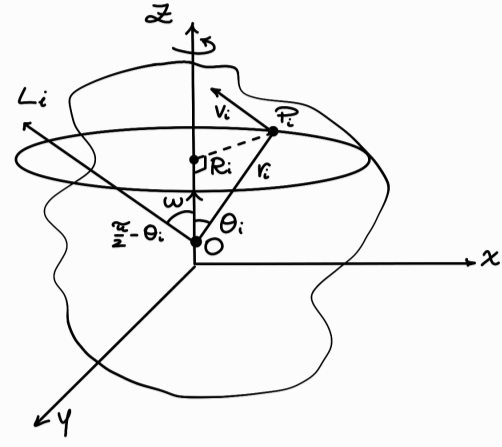
\includegraphics[width=0.5\linewidth]{Immagini/rotazioni rigide.png}
    \caption{vettore momento angolare per una rotazione rigida.}
    \label{fig: rotazione rigida}
\end{figure}

La proiezione angolare di $\vL_i$ sull'asse di rotazione, che prende il nome di momento assiale, è
\begin{equation}
    L_{iz}=L_i\cos{\bigg(\frac{\pi}{2}-\theta\bigg)}=L_i\sin{\theta_i}=m_ir_iR_i\omega\sin{\theta_i}=m_iR_i^2\omega.
\end{equation}
Il momento angolare del corpo è $\vL=\sum_i\vL_i$, e, in generale, non è parallelo all'asse di rotazione. Questo implica che in generale non esiste una proporzionalità tra $\vL$ e $\vom$. La proiezione di $\vL$ sull'asse $z$ è
\begin{equation}
    L_z=\nsum_iL_{iz}=\bigg(\nsum_im_iR_i^2\bigg)\omega=I_z\omega.
\end{equation}
Il coefficiente $I_z$ prende il nome di momento di inerziale del corpo rigido rispetto all'asse $z$ ed è appunto dato da
\begin{equation}
\label{eq: momento di inerzia discreto}
    I_z=\nsum_im_iR_i^2=\nsum_im_i(x_i^2+y_i^2).
\end{equation}
Il momento di inerzia dipende dalle masse e dalla loro posizione rispetto all'asse di rotazione: non è una caratteristica del corpo che si possa calcolare nota la sua struttura, ma per definirlo è necessario conoscere anche la posizione rispetto al corpo dell'asse di rotazione. Quindi, la componente parallela all'asse può variare solo in modulo, è proporzionale a $\omega$ e non dipende dalla scelta del polo. Invece, la componente ortogonale all'asse $L_\perp$ varia in direzione, in modulo e dipende dalla scelta del polo; questa corrisponde alla somma vettoriale di contributi, ognuno dei quali vale in modulo
\begin{equation}
    L_{i,\perp}=L_i\cos{\theta_i}=m_ir_iR_i\cos{\theta_i}.
\end{equation}
Il momento angolare $\vL$ è sicuramente parallelo all'asse di rotazione, e quindi ad $\vom$, quando l'asse di rotazione è un asse di simmetria, o, più in generale, quando l'asse di rotazione coincide con un asse principale di inerzia. In tali condizioni, si hanno
\begin{equation}
\label{eq: relazioni momento angolare per asse rot. = asse princip. inerzia}
    \vL=I_z\vom,\quad L=L_z,\quad L_\perp=0.
\end{equation}
Se $\vL$ è variabile, le variazioni $d\vL/dt$ sono anch'esse parallele a $\vom$ e quindi il momento delle forze esterne $\vM$ che le provoca è parallelo a $\vom$. Se invece $\vL$ è costante, ovvero $\vom$ è costante, il moto si svolge senza momento esterno, salvo la presenza di attrito. Nel caso più semplice in cui $\vL\parallel\vom$, valgono le \eqref{eq: relazioni momento angolare per asse rot. = asse princip. inerzia}, per cui
\begin{equation}
    \frac{d\vL}{dt}=\frac{d}{dt}(I_z\vom)=I_z\frac{d\vom}{dt}=I_z\valpha.
\end{equation}
Dunque, l'equazione del moto di rotazione è
\begin{equation}
\label{eq: moto rotazione asse rot. = asse princip. inerzia}
    \vM=I_z\valpha.
\end{equation}
Sia $\valpha$ che $\vM$ sono paralleli all'asse di rotazione, ossia a $\vom$. Note le condizioni iniziali, cioè la velocità e la posizione iniziali angolari, da \eqref{eq: moto rotazione asse rot. = asse princip. inerzia} si può ricavare la legge oraria, infatti
\begin{equation}
    \alpha=\frac{M}{I_z}\Rightarrow\omega(t)=\omega_0+\int_0^t\alpha\,dt\Rightarrow\theta(t)=\theta_0+\int_0^t\omega\,dt.
\end{equation}
Se $M=0$ il corpo resta in quiete o si muove con moto circolare uniforme, in particolare
\begin{equation}
    \alpha=0,\quad\omega=\omega_0,\quad\theta=\theta_0+\omega t.
\end{equation}
Se $M=costante$ il moto è circolare uniformemente accelerato, in particolare
\begin{equation}
    \alpha=costante,\quad\omega=\omega_0+\alpha t,\quad\theta=\theta_0+\omega_0t+\frac{1}{2}\alpha t^2.
\end{equation}
Infine, con $M$ generico, $\alpha=\alpha(t)$ e il moto è circolare vario. Per quanto riguarda in particolare il moto del centro di massa, se questo non sta sull'asse di rotazione, ma ne dista $R_{CM}$, l'accelerazione $\acm$ si calcolo a partire da $\alpha$ e $\omega$. In particolare, la componente tangente è $\acm^{T}=\alpha R_{CM}$, quella normale è $\acm^N=\omega^2R_{CM}$. La velocità è $\vcm=\omega R_{CM}$. Invece, l'energia cinetica del corpo rigido in rotazione è data da
\begin{equation}
\label{eq: energia cinetica rotazione corpo rigido}
    K=\nsum_i\frac{1}{2}m_iv_i^2=\nsum_i\frac{1}{2}m_iR_i^2\omega^2=\frac{1}{2}I_z\omega^2.
\end{equation}
Anche l'energia cinetica dipende dal momento di inerzia rispetto all'asse di rotazione. Se $\vL\parallel\vom$, allora da \eqref{eq: relazioni momento angolare per asse rot. = asse princip. inerzia} si ha
\begin{equation}
    K=\frac{L^2}{2I_z}.
\end{equation}
Quando un corpo rigido in quiete o in rotazione viene portato a ruotare con una velocità angolare $\omega_f$ tramite l'applicazione di un momento esterno, l'energia cinetica subisce una variazione e quindi è stato applicato un lavoro. Tale lavoro è dato da
\begin{equation}
\label{eq: lavoro rotazione corpo rigido}
    W=\Delta K=\frac{1}{2}I_z(\omega^2_f-\omega^2_i).
\end{equation}
Scrivendo questa equazione in forma infinitesima si ha
\begin{equation}
    dW=dK=I_z\omega\,d\omega=I_z\frac{d\theta}{dt}\alpha\,dt=I_z\alpha\,d\theta=M\,d\theta,
\end{equation}
la quale integrata dalla posizione iniziale a quella finale restituisce 
\begin{equation}
    W=\int_0^\theta M\,d\theta.
\end{equation}
Quindi, la potenza istantanea è
\begin{equation}
    P=\frac{dW}{dt}=M\frac{d\theta}{dt}=M\omega.
\end{equation}
Per eseguire il calcolo del lavoro è necessario conoscere la dipendenza angolare del momento.

Si noti che le formule \eqref{eq: relazioni momento angolare per asse rot. = asse princip. inerzia} e \eqref{eq: moto rotazione asse rot. = asse princip. inerzia} valgono solo se $\vL\parallel\vom$. In caso contrario, il vettore $\vL$ ruota intorno all'asse di rotazione descrivendo un moto di precessione, in particolare di precessione uniforme se $\vom$ è costante. In questo caso, l'equazione del moto \eqref{eq: eq. moto rotazione corpo rigido} ha due componenti 
\begin{equation}
    \vM_z=\frac{d\vL_z}{dt},\quad\vM_\perp=\frac{d\vL_\perp}{dt},
\end{equation}
essendo $\vM_z$ e $\vM_\perp$ la componente del momento angolare delle forze esterne $\vM$ parallela e perpendicolare all'asse di rotazione. La prima equazione corrisponde a \eqref{eq: moto rotazione asse rot. = asse princip. inerzia}, e da questa tramite $\alpha$ e le condizioni iniziali si ricava la legge oraria vista in precedenza: il moto di rotazione è ancora regolato da $M_z$. In particolare, se $M_z=0$, il corpo ruota con $\omega$ costante e $L_z$ è anch'esso costante. Invece, $L_\perp$ in ogni caso ruota assieme al corpo, potendo restare di modulo costante, se $\omega$ è costante, ma variando sempre in direzione. Le variazioni di $L_\perp$ sono regolate da $M_z$. In generale, la strada da seguire è:
\begin{quote}
    ``quando un corpo rigido ruota attorno ad una asse è conveniente mettersi in una situazione tale che $\vL$ e $\vom$ siano paralleli.''
\end{quote}
\begin{ex}
    Per capire l'origine di $M_\perp$ si può considerare un corpo rigido formato da due masse uguali $m$ collegate da un'asta rigida di massa trascurabile che forma un angolo $\theta$ con l'asse di rotazione. Questo ruota con velocità angolare $\vom$ e questo moto è dovuto ad un momento $M_z$, eventualmente nullo se $\vom$ è costante. D'altra parte, le due masse descrivono un moto circolare e per questo sono necessarie due forze centripete $\vF_C$, esercitate dell'asta. Queste due forze costituiscono una coppia e si dimostra che il momento è proprio $dL_\perp/dt$. Le due forze peso invece hanno momento nullo rispetto al polo $O$, come si deduce dalla figura \ref{fig: asta con masse}. 
    \begin{figure}[h]
        \centering
        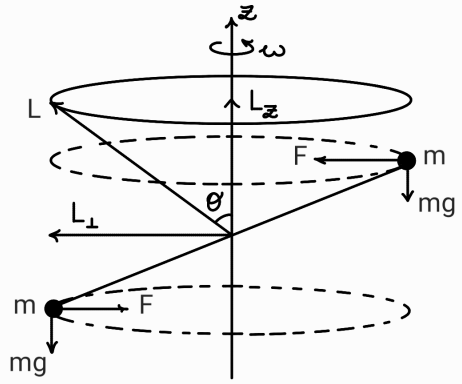
\includegraphics[width=0.5\linewidth]{Immagini/asta con masse.png}
        \caption{asta rigida in rotazione rigida.}
        \label{fig: asta con masse}
    \end{figure}
    Un effetto del momento delle $\vF_C$ è quello di far cambiare direzione all'asse di rotazione e quindi occorrono opportuni supporti in modo da mantenere l'asse in posizione verticale, i quali vengono sollecitati durante il moto. Se $\theta=\pi/2$, $\vL$ sarebbe parallelo a $\vom$ e questi effetti non si verificherebbero. 
\end{ex}
Per quanto riguarda energia cinetica e lavoro le equazioni \eqref{eq: energia cinetica rotazione corpo rigido} e \eqref{eq: lavoro rotazione corpo rigido} hanno validità generale. Invece, cambia il legame tra energia cinetica e momento angolare che diventa
\begin{equation}
    K=\frac{L_z^2}{2I_z}.
\end{equation}
Cambia anche l'espressione del lavoro tramite il momento $M_z$ che diventa
\begin{equation}
    W=\int_0^\theta M_z\,d\theta.
\end{equation}
Pertanto, quando $\vL$ non è parallelo a $\vom$, la legge oraria e il lavoro dipendono dalle componenti lungo l'asse di rotazione del momento angolare e del momento delle forze. Si vede come le corrispondenti formule nel caso del parallelismo tra $\vL$ e $\vom$ siano comprese nel caso generale, in quanto $M_z=M$ e $L_z=L$. 

\subsection{Momento di inerzia}
Il momento di inerzia ha un ruolo fondamentale, analogo a quello della massa nel secondo principio di Newton: a parità di momento applicato un corpo assume un'accelerazione angolare maggiore o minore a seconda del valore del momento di inerzia rispetto all'asse di rotazione. Tuttavia, c'è una profonda differenza tra i due concetti: mentre si può associare ad ogni corpo una massa, non ha senso parlare di momento di inerzia di un corpo di determinata forma, ma bisogna sempre specificare l'asse di rotazione a cui si fa riferimento. 

Il momento di inerzia di un corpo continuo si deduce da \eqref{eq: momento di inerzia discreto} effettuando il passaggio al continuo, quindi questo è
\begin{equation}
    I=\int R^2\,dm=\int_V\rho R^2\,dV=\int_V\rho(x^2+y^2)\,dV,
\end{equation}
dove $R$ è la distanza dell'elemento di massa $dm$ dall'asse $z$, assunto come asse di rotazione. Essendo il momento di inerzia additivo, se si suddivide un corpo in tante parti il momento di inerzia totale è la somma dei momenti di inerzia parziali, calcolati tutti rispetto allo stesso asse di rotazione. 
\begin{ex}
    Si consideri un disco omogeneo di massa $m$ e raggio $R$. La massa del disco è quindi esprimibile in termini di densità come $m=\rho_S\pi R^2$. Quindi, il momento di inerzia $I$ rispetto all'asse $z$ è
    \begin{equation}
        I_z=\int r^2\,dm=\int\rho_S r^2\,dS.
    \end{equation}
    Usando le coordinate polari $dS=r\,drd\phi$. Pertanto, si ha
    \begin{equation}
        I_z=\int\rho_S r^2\,dS=\rho_S\int_0^R\int_0^{2\pi}r^3\,drd\phi=\frac{1}{2}\pi\rho_SR^4=\frac{1}{2}mR^2.
    \end{equation}
\end{ex}
\begin{ex}
    Si consideri un'asta omogenea di massa $m$, lunghezza $d$ e sezione $S$. La massa dell'asta in termini di densità è $m=\rho Sd$, quindi un elemento infinitesimo a distanza $dx$ dall'asse è $dm=\rho S\,dx$. Quindi, il momento di inerzia rispetto ad un asse ortogonale all'asta passante per il suo centro è
    \begin{equation}
        I_z=\int_{-d/2}^{d/2}x^2\,dm=\rho S\int_{-d/2}^{d/2}x^2\,dx=\frac{1}{12}\rho Sd^3=\frac{1}{12}md^2.
    \end{equation}
    Invece, il momento di inerzia rispetto ad un asse passante per un estremo dell'asta è
    \begin{equation}
        I_z=\int_0^dx^2\,dm=\rho S\int_0^dx^2\,dx=\frac{1}{3}\rho Sd^3=\frac{1}{3}md^2.
    \end{equation}
\end{ex}
In generale, il momento di inerzia ha un'espressione del tipo 
\begin{equation}
    I=fmd^2,
\end{equation}
dove $m$ è la massa del corpo, $d$ una dimensione significativa (ad esempio il raggio per una sfera o la lunghezza per un'asta) e $f$ è un fattore numerico legato alla struttura del sistema. Pertanto, il momento di inerzia si può scrivere come
\begin{equation}
    I=mk^2,\quad k=d\sqrt{f}=\sqrt{\frac{I}{m}},
\end{equation}
dove $k$ è il raggio giratore del corpo. Dato un corpo con momento di inerzia $I$ rispetto ad un asse, si immagini di concentrarne la massa in un punto: $k$ rappresenta la distanza dall'asse a cui bisogna porre questo punto per avere lo stesso momento di inerzia $I$.

Se per il calcolo del momento di inerzia si dovesse scegliere un asse per il quale vengono meno le condizioni di simmetria, il calcolo dei vari integrali può risultare complicato. Il seguente teorema semplifica enormemente il problema. 
\begin{teo}[teorema di Huygens-Steiner]
    Il momento di inerzia di un corpo di massa $m$ rispetto ad un asse che si trova ad una distanza $a$ dal centro di massa del corpo è dato da
    \begin{equation}
        I=I_{CM}+ma^2,
    \end{equation}
    dove $I_{CM}$ è il momento d'inerzia del corpo rispetto ad un asse parallelo al primo e passante per il centro di massa.
\end{teo}
\begin{proof}
    In riferimento alla figura \ref{fig: THS proof}, si considerino due assi $z$ e $z'$, tra loro paralleli, distanti $a$. L'asse $z'$ passa per il centro di massa. La relazione tra le coordinate nei due sistemi, con centro in $O$ e nel centro di massa, è dato da
    \begin{equation}
        x=x',\quad y=y'+a,\quad z=z'.
    \end{equation}
    \begin{figure}[h]
        \centering
        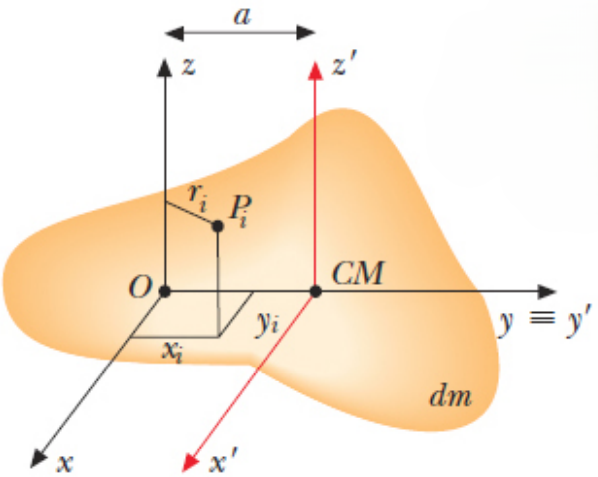
\includegraphics[width=0.4\linewidth]{Immagini/THS proof.png}
        \caption{schema per la dimostrazione del teorema di Huygens-Steiner.}
        \label{fig: THS proof}
    \end{figure}
    
    Il momento d'inerzia di un punto generico $P_i$ rispetto all'asse $z$ è dato da
    \begin{equation}
        I_{i}=m_i(x_i^2+y_i^2).
    \end{equation}
    Sommando su tutti i punti utilizzando le formule di trasformazione si ha
    \begin{equation}
        \begin{split}
            I_z&=\nsum_im_i(x_i^2+y_i^2)=\nsum_im_i[(x_i')^2+(y_i'+a)^2]\\
            &=\nsum_im_i[(x_i')^2+(y_i')^2]+\nsum_im_ia^2+2a\nsum_im_iy_i'.
        \end{split}
    \end{equation}
    Il primo termine è il momento di inerzia del corpo rispetto all'asse $z'$, il secondo è $ma^2$ e il terzo è nullo in quanto corrisponde a $m\ycm'$ e $\ycm'$, coordinata del centro di massa nel sistema del centro di massa, che è nulla. Si è quindi trovato
    \begin{equation}
         I_z=I_{z'}+ma^2=I_{CM}+ma^2.
    \end{equation}
\end{proof}
\begin{obs}
    Quindi $a$ non è altro che la distanza tra i due assi rispetto ai quali vengono calcolati i momenti d'inerzia.
\end{obs}
Si riconsideri l'equazione \eqref{eq: energia cinetica rotazione corpo rigido} e si applichi il teorema di Huygens-Steiner
\begin{equation}
    K=\frac{1}{2}(I_{CM}+ma^2)\omega^2=\frac{1}{2}I_{CM}\omega^2+\frac{1}{2}ma^2\omega^2.
\end{equation}
D'altra parte, $a\omega$ rappresenta la velocità $\vcm$, che percorre una traiettoria circolare di raggio $a$ rispetto all'asse $z$, quindi 
\begin{equation}
    K=\frac{1}{2}I_{CM}\omega^2+\frac{1}{2}m\vcm^{\ 2}.
\end{equation}
Questo risultato è in accordo con il secondo teorema di K\"onig e con le caratteristiche del moto di un corpo rigido: quando il centro di massa non è sull'asse di rotazione, l'energia cinetica è data dalla somma di $K'=I_{CM}\omega^2/2$, tipico della rotazione che costituisce il moto rispetto al centro di massa, e di $K_{CM}=m\vcm^{\ 2}/2$, energia cinetica del centro di massa. 

\subsection{Moto di puro rotolamento}
Si consideri la situazione in cui l'asse di rotazione non sia una asse materiale, ma un asse geometrico che si sposta insieme al corpo rigido. Questo si trova sopra ad un piano e si muove rispetto ad esso. Se le velocità di tutti i punti sono uguali tra loro e parallele al piano il moto è di traslazione. In generale, però il corpo in questione rotola sul piano e il punto di contatto $C$ ha velocità non nulla rispetto al piano, in tal caso il moto è di rotolamento e strisciamento. Se invece la velocità di $C$ è nulla, allora il moto è di puro rotolamento. 
\begin{figure}[h]
    \centering
    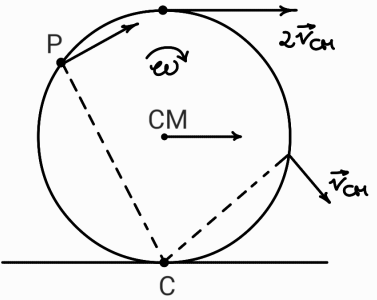
\includegraphics[width=0.4\linewidth]{Immagini/MPR.png}
    \caption{moto di puro rotolamento.}
    \label{fig: MPR}
\end{figure}
In ogni intervallo di tempo $dt$ il corpo che rotola senza strisciare può venir considerato come se ruotasse intorno ad un asse, fisso durante $dt$, passante per il punto di contatto $C$ e ortogonale al piano della figura \ref{fig: MPR}, con velocità angolare $\omega$. La velocità di ogni punto del corpo di conseguenza è ortogonale alla linea che congiunge $C$ con il punto ed è in modulo proporzionale alla distanza da $C$, quindi $v_P=\omega\overline{PC}$. In un intervallo successivo $dt$ il contatto avviene in un altro punto $C'$, infinitamente vicino $C$, e si ripete la rotazione attorno ad un altro asse fisso passante per $C'$, e così via. La velocità del punto $C$, distante $\vr$ dal centro di massa, si può sempre scrivere come $\vv_C=\vcm+\vom\times\vr$, mentre la condizione di puro rotolamento implica che $\vcm=-\vom\times\vr$. In modulo quindi si hanno
\begin{equation}
    v_{CM}=\omega r,\quad a_{CM}=\alpha r.
\end{equation}
Nel moto di puro rotolamento esiste una precisa relazione tra la velocità con cui avanza il centro di massa e  la velocità angolare, pertanto non sono indipendenti. Nel complesso la successione di rotazioni infinitesime attorno a $C$ equivale ad una rototraslazione in cui il centro di massa avanza con velocità $v_{CM}$ mentre il corpo ruota con velocità angolare $\omega$ rispetto ala centro di massa. 

Si consideri allora il caso di un corpo di massa $m$ e raggio $r$ che rotola senza strisciare su un piano orizzontale sotto l'azione di una forza orizzontale $\vF$ costante applicata all'asse. Sul corpo agisce anche la forza peso $m\vg$ e la reazione del piano $\vR$, che ha una componente normale $\vN$ e una tangenziale $\bm{f}$ corrispondente alla forza di attrito statico. La legge del moto del centro di massa è
\begin{equation}
    \vF+\vR+m\vg=m\acm,
\end{equation}
che proiettata sugli assi $x$ e $y$ restituisce rispettivamente
\begin{equation}
\label{eq: puro rot. 1}
    F-f=ma_{CM},\quad N=mg.
\end{equation}
Il teorema del momento angolare, scelto il centro di massa $O$ come polo, si scrive
\begin{equation}
    \vM=\vr\times\bm{f}=I\valpha,
\end{equation}
il cui modulo è
\begin{equation}
\label{eq: puro rot. 2}
     rf=I\alpha=I\frac{a_{CM}}{r}.
\end{equation}
Facendo sistema tra \eqref{eq: puro rot. 2} e la proiezione sull'asse $x$ \eqref{eq: puro rot. 1} si ricavano
\begin{equation}
    a_{CM}=\frac{F}{m\bigg(1+\dfrac{I}{mr^2}\bigg)},\quad f=\frac{F}{1+\dfrac{mr^2}{I}}.
\end{equation}
La forza $f$ non può assumere qualsiasi valore: non deve superare la massima forza di attrito statico, ovvero deve essere soddisfatta la disuguaglianza
\begin{equation}
    f\le\mu_sN=\mu_smg\Rightarrow F\le\mu_smg\bigg(1+\dfrac{mr^2}{I}\bigg)=F_{lim}.
\end{equation}
Pertanto, il moto può essere di puro rotolamento solo se la forza applicata non supera questa valore limite, altrimenti il corpo rotola e striscia. 

Invece di spingere il corpo, si può applicare all'asse un momento costante $\vM$. In questo caso, l'azione di $\vM$ tende a far slittare verso sinistra il punto di contatto e $\bm{f}$ è ora rivolta verso destra. Dalle equazioni
\begin{equation}
    \vR+m\vg=m\acm,\quad\vM+\vr\times\bm{f}=I\valpha,
\end{equation}
passando ai moduli si hanno
\begin{equation}
    N=mg,\quad f=ma_{CM},\quad M-rf=I\frac{a_{CM}}{r},
\end{equation}
da cui si ricavano
\begin{equation}
    a_{CM}=\frac{M}{mr^2\bigg(1+\dfrac{I}{mr^2}\bigg)},\quad f=\frac{M}{r\bigg(1+\dfrac{I}{mr^2}\bigg)}.
\end{equation}
Anche in questo caso si deve verificare
\begin{equation}
    f\le\mu_sN=\mu_smg\Rightarrow M\le\mu_smgr\bigg(1+\frac{I}{mr^2}\bigg)=M_{lim}.
\end{equation}
Mentre sotto l'azione di $\vF$ la reazione tangente $\bm{f}$ si oppone dal moto, a causa dell'azione di $\vM$, $\bm{f}$ favorisce il moto causando l'accelerazione del centro di massa. 

Nel caso più generale si ha l'azione contemporanea di una forza e di un momento. In tal caso non si può decidere a priori la direzione della forza $\bm{f}$, per cui la si assume parallela e concorde all'asse $x$. Le equazioni del moto sono
\begin{equation}
    F+f=ma_{CM},\quad M-rf=I\frac{a_{CM}}{r},
\end{equation}
da cui si ricavano
\begin{equation}
    a_{CM}=\frac{1}{m}\frac{F+\dfrac{M}{r}}{1+\dfrac{I}{mr^2}},\quad f=\frac{\dfrac{M}{r}-\dfrac{I}{mr^2}F}{1+\dfrac{I}{mr^2}}.
\end{equation}
con $f\le\mu_sN=\mu_smg$. La forza di attrito risulta concorde o discorde rispetto all'asse $x$ a seconda che $M$ sia maggiore o minore di $IF/mr$. In particolare, se $M=IF/mr$, la forza $f$ è nulla e $a_{CM}=F/m$: è possibile un moto accelerato anche in assenza di attrito. 

In conclusione, nel moto di rotolamento di un corpo rigido è possibile, con opportuni valori delle forze e dei momenti esterni, realizzare le condizioni per cui la reazione del piano è tale da mantenere fermo il punto di contatto., così che il corpo rotola senza strisciare. 

\subsubsection{Conservazione dell'energia e attrito volvente}
Al moto di puro rotolamento sotto l'azione di forze conservative si può applicare il principio di conservazione dell'energia meccanica. Infatti, la forza di attrito, che è normalmente diversa da zero, agisce su un punto fermo per cui lo spostamento è nullo e quindi è nullo il lavoro. Tuttavia, la conservazione dell'energia meccanica è un caso limite: sperimentalmente un corpo che rotola senza strisciare, in assenza di forze e momenti applicati, si arresta dopo un certo tempo. Pertanto, esiste un'altra forma di attrito, detta attrito volvente, che viene attribuito alla deformazione locale del piano ed è schematizzato con l'azione di un momento $M_v=hmg$ che si oppone al moto, dove $h$ è il coefficiente di attrito volvente. Per vincere tale momento, si deve applicare al corpo di massa $m$ e raggio $r$ una forza di trazione tale che $F\ge hmg/r$.
\begin{obs}
    Dato che l'effetto dell'attrito volvente è minimo rispetto a quello radente e dinamico, nel seguito lo si trascura.
\end{obs}

\subsection{Impulso angolare}
Come visto, la forma integrale del secondo principio di Newton è esprimibile tramite il teorema dell'impulso: l'impulso della forza è uguale alla variazione della quantità di moto. In modo analogo, si deduce il seguente teorema.
\begin{teo}[teorema dell'impulso angolare]
    L'azione di un momento durante un intervallo finito di tempo causa una variazione finita del momento angolare
    \begin{equation}
        \int_{t_1}^{t_2}\vM\,dt=\vL(t_2)-\vL(t_1)=\Delta\vL.
    \end{equation}
\end{teo}
Un modo per mettere in rotazione un corpo rigido rispetto ad un asse fisso consiste nell'applicazione di una forza intensa per un tempo molto breve in un dato punto. Prendendo come polo il punto di sospensione $O$ del corpo si ha
\begin{equation}
    \int\vM\,dt=\int(\vr\times\vF)\,dt=\vr\times\int\vF\,dt=\vr\times\vJ=\Delta\vL.
\end{equation}
Quindi, l'applicazione dell'impulso provoca, oltre ad una variazione di quantità di moto, una variazione di momento angolare uguale al momento dell'impulso. Si noti che nell'integrale non compaiono le forze di attrito, dato che hanno momento nullo in quanto applicate in $O$, e nemmeno la forza peso in quanto si assume trascurabile il suo impulso angolare rispetto a quello di $\vF$.
\begin{obs}
    Si erano già trovate espressioni analoghe e formalmente identiche per il punto materiale. La principale differenza sta nell'espressione del momento angolare.
\end{obs}

\subsection{Leggi di conservazione}
Se la risultante delle forze esterne è nulla, il centro di massa si muove di moto rettilineo uniforme, ma il moto dei singoli punti non è detto sia traslatorio rettilineo uniforme. In tal caso, la quantità di moto $\vp$ è costante e di conseguenza anche $\vcm$ è costante, con $\vp=m\vcm$. 

Assumendo come polo un punto fisso in un sistema di riferimento inerziale o il centro di massa, se $\vM=0$, allora il momento angolare $\vL$ resta costante in modulo, direzione e verso. Questo però non comporta $\vom=costante$, in quanto non è detto che il moto di rotazione avvenga attorno ad un asse principale di inerzia, ovvero che sia $\vL=I\vom$.

La legge di conservazione dell'energia meccanica nel moto di un corpo è valida quando non ci sono attriti o quando, come nel moto di puro rotolamento, le forze di attrito non compiono lavoro, pur essendo presenti. Inoltre, le reazioni vincolari che tengono fissi uno o più punti, non compiono lavoro, mentre la presenza di momenti di attrito che agiscono sull'asse di rotazione determina un lavoro che provoca una diminuzione dell'energia meccanica. 

\subsection{Equilibrio statico}
La condizione di equilibrio statico per un punto materiale è che la risultante delle forze applicate al punto sia nulla, ossia $\vR=0$. Se il punto è inizialmente in quiete, rimane in tale stato. Per un corpo rigido inizialmente in quiete si ha l'equilibrio statico se
\begin{equation}
    \vR=0,\quad\vM=0.
\end{equation}
La prima realizza l'equilibrio statico del centro di massa, ossia $\vcm=0$, mentre con la seconda non si ha moto rotatorio, ossia $\vom=0$. In questo caso, $\vM$ è indipendente dal polo, quindi se quest'ultimo è nullo rispetto ad un polo, lo è rispetto a qualsiasi altro. 

Si consideri infine l'equilibrio dei corpi sospesi, tipo pendolo composto, sottoposti alla forza peso. In qualsiasi posizione in cui il centro di massa non si trova sulla verticale passante per il centro di sospensione $O$, il momento della forza peso rispetto ad $O$ è diverso da zero e si compone di un'accelerazione angolare. Il centro di massa ha accelerazione diversa da zero, determinata dalla risultante della forza peso e della reazione vincolare in $O$. In tal caso non può esserci equilibrio statico se non agiscono altre forze. Se invece il centro di massa sta sulla verticale passante per $O$ e ha velocità nulla, la posizione è di equilibrio: il momento è nullo e la risultante delle forze è nulla (la reazione vale $m\vg$). Ci sono due posizioni possibili di questo tipo: il centro di massa sta sotto oppure sopra $O$. Nel primo caso se si allontana il corpo dalla posizione di equilibrio la forza peso tende a riportarlo, per cui l'equilibrio è stabile; nel secondo caso, il corpo si allontana ulteriormente dalla posizione di equilibrio, la forza peso lo fa ruotare portandolo verso il basso con il centro di massa sotto $O$, per cui l'equilibrio è instabile. Se il centro di sospensione coincide con il centro di massa, il momento della forza peso sarebbe sempre nullo e il corpo starebbe in quiete in qualsiasi posizione angolare: l'equilibrio è indifferente. 
\chapter{Fenomeni d'urto}
Si consideri l'urto tra due punti materiali. Durante il fenomeno si possono sviluppare forze molto intense che modificano la quantità di moto di ciascun punto. Queste forze, che agiscono per un breve intervallo di tempo rispetto a quello di osservazione del fenomeno, prendono il nome di forze impulsive. L'azione della forza si esplica nell'intervallo $\tau=t_1-t_1$. Le forze che si manifestano durante il processo d'urto sono forze interne. Quindi, in assenza di forze esterne, durante l'urto si verifica la conservazione della quantità di moto totale.

Indicando con $\vv_{1,i}$ e $\vv_{2,i}$ le velocità nell'istante precedente all'urto dei due punti materiali, di masse $m_1$ e $m_2$, e con $\vv_{1,f}$ e $\vv_{2,f}$ le corrispondenti velocità successive all'urto, la conservazione di $\vp$ si esprime come
\begin{equation}
    \vp_i=m_1\vv_{1,i}+m_2\vv_{2,i}=m_1\vv_{1,f}+m_2\vv_{2,f}=\vp_f.
\end{equation}
La quantità di moto del centro di massa rimane invariata
\begin{equation}
\label{eq: conservazione impulso CM urto 2 punti}
    \vp=(m_1+m_2)\vcm=\vp_i=\vp_f=costante.
\end{equation}
Quindi, il moto del centro di massa non viene modificato dall'urto dei due punti. Invece, variano le quantità di moto di ciascun punto materiale per effetto dell'impulso della forza di interazione secondo
\begin{align}
    \Delta\vp_1&=m_1\vv_{1,f}-m_1\vv_{1,i}=\int_{t_1}^{t_2}\vF_{2,1}\,dt=\vJ_{2,1} \\
    \Delta\vp_2&=m_1\vv_{2,f}-m_1\vv_{2,i}=\int_{t_1}^{t_2}\vF_{1,2}\,dt=\vJ_{1,2}.
\end{align}
Naturalmente
\begin{equation}
    \vF_{1,2}=-\vF_{2,1}\Rightarrow\vJ_{1,2}=-\vJ_{2,1},\quad\Delta\vp_1=-\Delta\vp_2,
\end{equation}
ossia le variazioni di quantità di moto sono uguali e opposte. 

Si può conservare la quantità di moto totale se sono presenti forze esterne? La risposta è sì se la durata dell'urto $\tau$ è sufficientemente breve e se le forze esterne non sono impulsive. Infatti, la variazione di $\Delta\vp$ in presenza di forze esterne è
\begin{equation}
\begin{split}
    \Delta\vp&=\Delta\vp_1+\Delta\vp_2=\int_{t_1}^{t_2}(\vF_{2,1}+\vF^{ext}_1)\,dt+\int_{t_1}^{t_2}(\vF_{1,2}+\vF^{ext}_2)\,dt \\
    &=\vJ_{2,1}+\vJ_{1,2}+\int_{t_1}^{t_2}\vF^{ext}\,dt=\vmedio{\vF^{ext}}\tau,
\end{split}
\end{equation}
dove se $\tau\to0$, allora anche $\Delta\vp\to0$. Se invece $\vF^{ext}$ fosse impulsiva in $\tau$, il valore medio $\vmedio{\vF^{ext}}$ potrebbe assumere valori molto alti, rendendo $\Delta\vp$ non trascurabile. La forza esterna non modifica i singoli impulsi durante l'urto quindi rimane vera l'uguaglianza $\vJ_{1,2}=-\vJ_{2,1}$ e quindi la conservazione della quantità di moto totale. Riassumendo, un urto è definito dalle seguenti proprietà:
\begin{enumerate}
    \item consiste in uno scambio di quantità di moto tra due punti materiali sotto forma di impulsi dovuti alle forze interne tra di essi;
    \item la quantità di moto totale si conserva.
\end{enumerate}
Queste caratteristiche prescindono dal meccanismo con il quale avviene l'urto e quindi dall'effettivo contatto tra i due punti. 

Tuttavia, a priori non è possibile sapere se le forze interne sono conservative e pertanto non si può applicare il principio di conservazione dell'energia meccanica. Dato che la posizione dei due punti durante l'urto non varia, le rispettive energie potenziali non variano e quindi $\Delta E=\Delta K$. Applicando il secondo teorema di K\"onig si ha
\begin{equation}
    K=\frac{1}{2}(m_1+m_2)\vcm^{\ 2}+K'.
\end{equation}
Il primo termine è l'energia cinetica del centro di massa, la quale non varia se si conserva la quantità di moto totale, mentre il secondo termine è l'energia cinetica rispetto al centro di massa, la quale può variare o meno a seconda che le forze interne siano non conservative o conservative, definita da
\begin{equation}
    K'=\frac{1}{2}m_1(v_1')^2+\frac{1}{2}m_2(v_2')^2.
\end{equation}

\section{Sistemi di laboratorio e centro di massa}
Per studiare gli urti i sistemi di riferimento più comuni sono quello del laboratorio e quello del centro di massa. Il legame tra le velocità in qualsiasi istante tra questi due è
\begin{equation}
\label{eq: legame velocità SdRL e SdRCM}
    \vv_1=\vvi_1+\vcm,\quad\vv_2=\vvi_2+\vcm.
\end{equation}
Nel sistema del centro di massa la quantità di moto totale è nulla, infatti, da $\vp=m_1\vv_1+m_2\vv_2$, usando \eqref{eq: conservazione impulso CM urto 2 punti} e \eqref{eq: legame velocità SdRL e SdRCM}, si ha
\begin{equation}
    \begin{split}
            \vp&=m_1\vvi_1+m_2\vvi_2+(m_1+m_2)\vcm\Rightarrow m_1\vvi_1+m_2\vvi_2=\vpi=0.
    \end{split}
\end{equation}
Quindi, da
\begin{equation}
    m_1\vvi_{1,i}+m_1\vvi_{2,i}=m_1\vvi_{1,f}+m_2\vvi_{2,f}=0,
\end{equation}
si ha
\begin{equation}
    \vpi_{1,i}=-\vpi_{2,i},\quad\vpi_{1,f}=-\vpi_{2,f}.
\end{equation}
Dunque, dal sistema del centro di massa, si osservano i punti materiali arrivare verso il centro di massa con quantità di moto uguali in modulo e opposte in verso, si urtano nella posizione occupata da quest'ultimo e ripartono nuovamente con quantità di moto uguali in modulo e opposte in verso, pur se in generale $\vpi_f\neq\vpi_i$. Da \eqref{eq: conservazione impulso CM urto 2 punti} si ha che la velocità del centro di massa è
\begin{equation}
\label{eq: velocità CM}
    \vcm=\frac{\vp}{m_1+m_2}=\frac{m_1\vv_1+m_2\vv_2}{m_1+m_2}.
\end{equation}
Sostituendo questa in \eqref{eq: legame velocità SdRL e SdRCM} si ottengono le velocità dei due punti nel sistema del centro di massa
\begin{equation}
\label{eq: velocità nel SdRCM}
    \vvi_1=\frac{m_2(\vv_1-\vv_2)}{m_1+m_2},\quad\vvi_2=\frac{m_1(\vv_2-\vv_1)}{m_1+m_2}.
\end{equation}
L'energia cinetica nel sistema del centro di massa coincide con quella relativa al centro di massa e in generale si ha $K_i\neq K_f$. 

\section{Urto completamente anelastico}
Un urto è completamente anelastico se i due punti materiali rimangono a contatto in seguito al fenomeno d'urto, formando un unico punto materiale di massa $m_1+m_2$. Se $\vv_1$ e $\vv_2$ sono le velocità dei due punti nell'istante prima dell'urto e $\vvi$ è la velocità comune in seguito a quest'ultimo, dalla conservazione della quantità di moto e \eqref{eq: conservazione impulso CM urto 2 punti}, si ha
\begin{equation}
    m_1\vv_1+m_2\vv_2=(m_1+m_2)\vvi=(m_1+m_2)\vcm,
\end{equation}
da cui
\begin{equation}
    \vcm=\frac{m_1\vv_1+m_2\vv_2}{m_1+m_2}.
\end{equation}
Quindi, in seguito all'urto i due punti si muovono congiuntamente con la velocità che il centro di massa aveva prima dell'urto, in quanto è costante durante il processo. 
\begin{figure}[h]
    \centering
    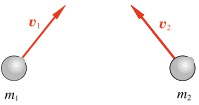
\includegraphics[width=0.41\linewidth]{Immagini/UCA 1.png}
    \quad
    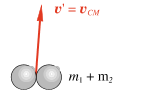
\includegraphics[width=0.3\linewidth]{Immagini/UCA 2.png}
    \caption{prima e dopo un urto completamente anelastico.}
    \label{fig: uerto completamente anelastico}
\end{figure}

Invece, l'energia cinetica prima dell'urto, applicando il secondo teorema di K\"onig, è
\begin{equation}
    K_i=\frac{1}{2}m_1v_1^2+\frac{1}{2}m_2v_2^2=K'+\frac{1}{2}(m_1+m_2)\vcm^{\ 2},
\end{equation}
mentre dopo l'urto è
\begin{equation}
    K_f=\frac{1}{2}(m_1+m_2)\vcm^{\ 2}<K_i.
\end{equation}
In effetti, dopo l'urto non è più presente moto rispetto al centro di massa, con cui i due punti coincidono, e pertanto si deduce che l'energia assorbita in questo tipo d'urto è $K'$, ossia l'energia cinetica i punti hanno rispetto al centro di massa prima dell'urto. La differenza di energia cinetica è infatti
\begin{equation}
    \Delta K=K_f-K_i=-K'.
\end{equation}
Dunque, le forze interne che si sviluppano in questo tipo di urto non sono conservative. 

\section{Urto elastico}
Un urto è elastico se nel processo si conserva anche l'energia meccanica del sistema. Questo implica necessariamente che le forze interne siano conservative. In questo tipo di urto si possono usare le relazioni
\begin{equation}
\label{eq: leggi di conservazione urto elastico}
    \vp_i=\vp_f,\quad K_i=K_f.
\end{equation}
Si consideri un urto elastico su un bersaglio nel piano. Nel sistema di riferimento del laboratorio e nel sistema di riferimento del centro di massa si hanno le situazioni mostrate in figura \ref{fig: urto elastico}.
\begin{figure}[h]
    \centering
        \begin{subfigure}{0.45\textwidth}
        \centering
        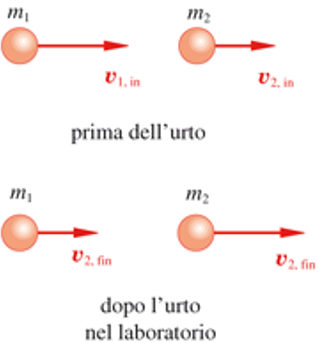
\includegraphics[width=0.8\linewidth]{Immagini/UEL.png}
        \end{subfigure}
    \quad
        \begin{subfigure}{0.45\textwidth}
        \centering
        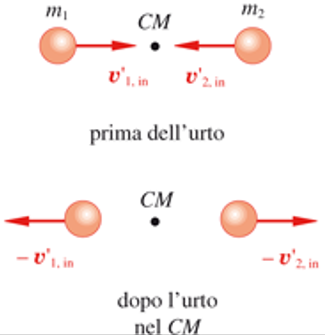
\includegraphics[width=0.8\linewidth]{Immagini/UECM.png}
        \end{subfigure}
    \caption{situazione prima e dopo l'urto nel sistema di riferimento del (i) laboratorio; (ii) centro di massa.}
    \label{fig: urto elastico}
\end{figure}

Si impongano le condizioni \eqref{eq: leggi di conservazione urto elastico} nel sistema di riferimento del laboratorio
\begin{equation}
    \begin{cases}
        \vp_{1,i}=\vp_{1,f}+\vp_{2,f} \\
        K_{1,i}=K_{1,f}+K_{2,f}
    \end{cases},
\end{equation}
che, esplicitando in termini di massa e velocità, diventano
\begin{equation}
    \begin{cases}
        m_1\vv_{1,i}=m_1\vv_{1,f}+m_2\vv_{2,f} \\[1.5ex]
        \dfrac{1}{2}m_1v_{1,i}^2=\dfrac{1}{2}m_1v_{1,f}^2+\dfrac{1}{2}m_2v_{2,f}^2
    \end{cases}.
\end{equation}
Scomponendo le velocità della prima equazione sugli assi cartesiani si ottengono
\begin{equation}
    \begin{cases}
        m_1v_{1,i}=m_1v_{1,fx}+m_2v_{2,fx} \\
        0=m_1v_{1,fy}+m_2v_{2,fy}
    \end{cases}.
\end{equation}
Quindi, si ottengono tre equazioni in quattro incognite, che sono le componenti $x$ e $y$ di $\vv_{1,f}$ e $\vv_{2,f}$. Non tutto è determinato a priori, ma c'è una dipendenza da un parametro libero che può essere identificato nell'angolo $\theta'$ di diffusione nel sistema di riferimento del centro di massa. 

Quindi, ponendosi nel sistema del centro di massa, si possono scrivere le condizioni \eqref{eq: leggi di conservazione urto elastico} come
\begin{equation}
    \begin{cases}
        m_1\vv_{1,i}'+m_2\vv_{2,i}'=m_1\vv_{1,f}'+m_2\vv_{2,f}'=0 \\[1.5ex]
        \dfrac{1}{2}m_1(\vvi_{1,i})^2+\dfrac{1}{2}m_2(\vvi_{2,i})^2=\dfrac{1}{2}m_1(\vvi_{1,f})^2+\dfrac{1}{2}m_2(\vvi_{2,f})^2
    \end{cases}.
\end{equation}
Si dimostra ora che le velocità rimangono invariate in modulo e possono ruotare solo di un angolo $\theta'$, ossia che
\begin{equation}
    v'_{1,i}=v_{1,f}',\quad v_{2,i}'=v_{2,f}'.
\end{equation}
Dalla prima equazione del sistema precedente si ottengono
\begin{equation}
    \begin{cases}
        m_1\vv_{1,i}'=-m_2\vv_{2,i}' \\
        m_1\vv_{1,f}'=-m_2\vv_{2,f}'
    \end{cases},
\end{equation}
e, se si considerano i moduli, si ottengono
\begin{equation}
    \begin{cases}
    \label{eq: sistema dimostrazione velocità urto elastico}
        v_{1,i}'=\dfrac{m_2}{m_1}v_{2,i}' \\[1.5ex]
        v_{1,f}'=\dfrac{m_2}{m_1}v_{2,f}'
    \end{cases}.
\end{equation}
Sostituendo queste nell'equazione di conservazione dell'energia cinetica si ottiene
\begin{equation}
    \begin{split}
        \dfrac{1}{2}m_1\bigg(\dfrac{m_2}{m_1}v_{2,i}'\bigg)^2+\dfrac{1}{2}m_2(\vvi_{2,i})^2&=\dfrac{1}{2}m_1\bigg(\dfrac{m_2}{m_1}v_{2,f}'\bigg)^2+\dfrac{1}{2}m_2(\vvi_{2,f})^2 \\
        \dfrac{1}{2}v_{2,i}^2\bigg(\frac{m_2^2}{m_1}+m_2\bigg)&=\dfrac{1}{2}v_{2,f}^2\bigg(\frac{m_2^2}{m_1}+m_2\bigg) \\
        (v_{2,i}')^2&=(v_{2,f}')^2 \\
        v_{2,i}'&=v_{2,f}'.
    \end{split}
\end{equation}
Sostituendo questo risultato in \eqref{eq: sistema dimostrazione velocità urto elastico} si ottiene
\begin{equation}
    v_{1,i}'=v_{1,f}'.
\end{equation}
Si è quindi dimostrato che, nel sistema del centro di massa, i modulo delle velocità sono uguali prima e dopo l'urto. Quindi, i vettori velocità possono solo ruotare di un angolo $\theta'$. Si studia ora l'urto nel sistema del centro di massa.

Prima dell'urto il centro di massa si muove solo lungo la direzione delle $x$. Usando le equazioni \eqref{eq: velocità CM} e \eqref{eq: velocità nel SdRCM}, e imponendo che il secondo corpo prima dell'urto è fermo, si ottengono
\begin{equation}
    \begin{cases}
        v_{CM}=\dfrac{m_1}{m_1+m_1}v_{1,i} \\[1.5ex]
        v_{1,i}'=\dfrac{m_2}{m_1+m_2}v_{1,i}<v_{1,i} \\[1.5ex]
        v_{2,i}'=-\dfrac{m_1}{m_1+m_2}v_{1,i}=-v_{CM}
    \end{cases}.
\end{equation}
Sostituendo la seconda equazione di questo sistema in $v_{1,i}'=v_{1,f}'$ si ottiene
\begin{equation}
    v_{1,i}'=v_{1,f}'=\dfrac{m_2}{m_1+m_2}v_{1,i}=\dfrac{m_2}{m_1+m_2}\dfrac{m_1+m_2}{m_1}v_{CM}=\frac{m_2}{m_1}v_{CM}.
\end{equation}
In modulo, usando l'equazione $v_{2,i}'=v_{2,f}'$ e l'ultima equazione del medesimo sistema si ottiene
\begin{equation}
    v_{2,i}'=v_{2,f}'=v_{CM}.
\end{equation}
Rispetto al moto del centro di massa, il primo e il secondo corpo si muovono con un angolo $\theta'$ e le loro velocità sono
\begin{equation}
    \begin{cases}
        v_{1,fx}'=\dfrac{m_2}{m_1}v_{CM}\cos{\theta'} \\[1.5ex]
        v_{1,fy}'=\dfrac{m_2}{m_1}v_{CM}\sin{\theta'}
    \end{cases},\quad
    \begin{cases}
        v_{2,fx}'=-v_{CM}\cos{\theta'} \\
        v_{2,fy}'=-v_{CM}\sin{\theta'}
    \end{cases},
\end{equation}
dove per il secondo corpo si sono usate le relazioni in \eqref{eq: sistema dimostrazione velocità urto elastico}. 

Ora passando al sistema di riferimento del laboratorio, usando l'equazione $m_1\vv_{1,i}=m_1\vv_{1,f}+m_2\vv_{2,f}$, per la situazione dopo l'urto si ha
\begin{equation}
    \begin{cases}
        v_{1,fx}=v_{CM}+\dfrac{m_2}{m_1}v_{CM}\cos{\theta'} \\
        v_{1,fy}=\dfrac{m_2}{m_1}v_{CM}\sin{\theta'}
    \end{cases},
\end{equation}
che implica, usando \eqref{eq: sistema dimostrazione velocità urto elastico}, per il secondo corpo
\begin{equation}
    \begin{cases}
        v_{2,fx}=v_{CM}(1-\cos{\theta'}) \\
        v_{2,fy}=-v_{CM}\sin{\theta'}
    \end{cases}.
\end{equation}
Il sistema del primo corpo descrive l'equazione di una circonferenza centrata in $v_x=v_{CM}$ e di raggio $r=(m_2/m_1)v_{CM}$, mentre il sistema del secondo corpo descrive l'equazione di una circonferenza centrata in $v_x=v_{CM}$ e di raggio $r=v_{CM}$. In particolare, queste sono
\begin{equation}
    \begin{cases}
        (v_{1,fx}-v_{CM})^2+(v_{1,fy}^2)=\bigg(\dfrac{m_2}{m_1}v_{CM}\bigg)^2 \\[1.5ex]
        (v_{2,fx}-v_{CM})^2+(v_{2,fy})^2=(v_{CM})^2
    \end{cases}.
\end{equation}
Si presentano tre casi:
\begin{enumerate}
    \item Se il bersaglio è pesante, ossia $m_2>m_1$, allora il proiettile può tornare indietro (Rutherford).
    \item Se il bersaglio ha la stessa massa del proiettile, ossia $m_1=m_2$, allora il proiettile può fermarsi (Fermi).
    \item Se il bersaglio è leggero, ossia $m_1>m_2$, allora il proiettile non torna mai indietro, ma solo in avanti.
\end{enumerate}

\section{Urto anelastico}
Il caso di urto più comune si verifica quando i due punti materiali, dopo aver colliso, tornano ad essere separati. Se non agiscono forze esterne di tipo impulsivo, la quantità di moto si conserva, ma non l'energia cinetica. Una certa frazione $K'$, l'energia cinetica prima dell'urto rispetto al centro di massa, viene assorbita. 


Si consideri un urto elastico nel sistema di riferimento del centro di massa. Il punto con quantità di moto $\vpi_{1,i}$ nell'istante precedente all'urto vede, per effetto dell'impulso nella fase di deformazione, ridursi la quantità di moto progressivamente a zero fino ad arrestarsi. Nella fase successiva, sempre durante l'urto, il punto riacquista quantità di moto fino al valore $\vpi_{1,f}$, opposto in verso e minore di $\vpi_{1,i}$. Si definisce il coefficiente di restituzione $\epsilon$ il rapporto
\begin{equation}
    \epsilon=-\frac{\vpi_{1,f}}{\vpi_{1,i}}=-\frac{\vvi_{1,f}}{\vvi_{1,i}}=-\frac{\vpi_{2,f}}{\vpi_{2,i}}=-\frac{\vvi_{2,f}}{\vvi_{2,i}}.
\end{equation}
Infatti, dato che $\vp=0$, in modulo $p_{1,i}'=p_{2,i}'$ e $p_{1,f}'=p_{2,f}'$, per cui il coefficiente di restituzione è lo stesso anche per la seconda particella. L'energia cinetica del sistema delle due particelle dopo l'urto è
\begin{equation}
    K_f'=\frac{1}{2}m_1(v'_{1,f})^2+\frac{1}{2}m_2(v'_{2,f})^2=\epsilon^2\bigg[\frac{1}{2}m_1(v'_{1,i})^2+\frac{1}{2}m_2(v'_{2,i})^2\bigg]=\epsilon^2K_i'.
\end{equation}
La variazione relativa di energia cinetica rispetto al centro di massa nell'urto è
\begin{equation}
    \delta=\frac{K_f'-K_i'}{K_i'}=\epsilon^2-1.
\end{equation}
Nell'urto elastico $\epsilon=1$ e $\delta=0$, nell'urto completamente anelastico $\epsilon=0$ e $\delta=-1$. Nella situazione di urto anelastico, il coefficiente di restituzione risulta $\epsilon\in(0,1)$, mentre $K_f'<K_i'$. 

La soluzione per le velocità finali nel sistema di riferimento inerziale, sempre nel caso di urto centrale come per l'urto elastico, risulta
\begin{align}
    v_{1,f}&=\frac{(m_1-\epsilon m_2)v_{1,i}+m_2(1+\epsilon)v_{2,i}}{m_1+m_2}, \\
    v_{2,f}&=\frac{m_1(1+\epsilon)v_{1,i}+(m_2-\epsilon m_1)v_{2,i}}{m_1+m_2}.
\end{align}
Con $\epsilon=1$ e $\epsilon=0$ si ritrovano infatti le relazioni per il caso elastico e completamente anelastico. 

\section{Urto con corpi rigidi}
Un urto può anche avvenire tra un punto materiale e un corpo rigido oppure tra due (o più) corpi rigidi. Riassumendo, in un urto si può assumere la costanza dell'energia cinetica del sistema solo se è noto a priori che l'urto è elastico. Se agiscono solo forze interne, o quelle esterne non sono di tipo impulsivo, si conserva la quantità di moto totale. Se invece esiste un vincolo che tiene fermo un punto del corpo rigido, e quindi sviluppa una forza esterna di tipo impulsivo durante l'urto, non si verifica la conservazione della quantità di moto. Infine, qualora rispetto a un certo polo, fisso in un sistema di riferimento inerziale o coincidente con il centro di massa, il momento delle forze esterne, comprese quelle vincolari è nullo, si  conserva il momento angolare rispetto a tale polo. Se agiscono solo forze interne $\vL$ si conserva sempre, indipendentemente dalla scelta del polo.

Quando il corpo urtato è vincolato, il sistema di vincoli può esplicare durante l'urto un sistema di forze che ha una risultante $\vR$ e un momento risultante $\vM$. L'effetto complessivo, nel brevissimo tempo di durata dell'urto, è dato dall'impulso della forza $J=\int\vR\,dt$ e dall'impulso angolare $\Delta L=\int\vM\,dt$, eguali rispettivamente alla variazione della quantità di moto e alla variazione del momento angolare del sistema.

Essendo la quantità di moto e il momento angolare grandezze vettoriali, è possibile trovare situazioni in cui la loro conservazione è parziale; per esempio, $p_x$ e $p_y$ si conservano, $p_z$ cambia: questo vuol dire che l'impulso ha componenti $J_x$ e $J_y$ nulle, mentre $J_z$ è diversa da zero. Analogamente per $\vL$ e l'impulso angolare.
\begin{figure}[h]
    \centering
    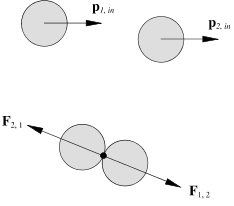
\includegraphics[width=0.3\linewidth]{Immagini/UCR 1.png}
    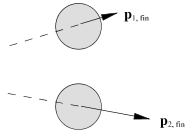
\includegraphics[width=0.3\linewidth]{Immagini/UCR 2.png}
    \caption{urto tra due corpi rigidi non ruotanti (i) prima dell'urto; (ii) durante l'urto; (iii) dopo l'urto.}
    \label{fig: urto corpi rigidi}
\end{figure}

Quando due corpi estesi si urtano, ma non restano attaccati, le quantità di moto dopo l'urto formano normalmente un certo angolo con la direzione che avevano prima dell'urto. Infatti la forza interna impulsiva $\vF_{2,1}$ agente sul primo corpo non è parallela a $\vp_{1,i}$ e quindi $\vp_{1,f}$ risulta deviata rispetto alla direzione iniziale del moto; lo stesso succede per il secondo corpo. La situazione è mostrata qualitativamente in figura \ref{fig: urto corpi rigidi} riferita a due dischetti che non ruotano prima dell'urto. Essi non ruotano nemmeno dopo se non c'è attrito al contatto, cioè se le forze interne non hanno componente tangente. Altrimenti il momento dell'attrito mette in rotazione i dischetti. Solo se i centri dei due dischetti si muovono lungo la stessa retta non si ha deviazione e si parla di urto centrale; l'urto della \ref{fig: urto corpi rigidi} non è centrale.
\chapter{Gravitazione}
Agli inizi del Cinquecento, Copernico avanzò l'ipotesi eliocentrica: il Sole, e non la Terra, era il corpo celeste attorno al quale si svolgeva il moto dei pianeti. Alla fine del secolo, le posizioni da lui assunte erano state oggetto di numerose misurazioni da parte di Brahe. Proprio su queste misure, agli inizi del Seicento, si basò Keplero per formulare le sue tre leggi.
\begin{teo}[leggi di Keplero]\hfill
    \begin{enumerate}
        \item I pianeti percorrono orbite ellittiche intorno al sole che occupa uno dei due fuochi.
        \item La velocità areale con cui il raggio vettore che unisce il Sole ad un pianeta descrive l'orbita è costante.
        \item Il quadrato del periodo di rivoluzione $T$ di ogni pianeta è proporzionale al cubo del semiasse maggiore dell'ellisse $a$, ossia $T^2=ka^3$.
    \end{enumerate}
\end{teo}
Le tre leggi di Keplero forniscono una descrizione cinematica del moto dei pianeti. La spiegazione dinamica venne trovata da Newton nel 1666 e resa nota solo nel 1687. Questa fu l'origine della Teoria della gravitazione universale.

\section{Forza gravitazionale}
Il ragionamento di Newton per determinare l'origine dinamica del moto dei pianeti, inizialmente approssimato, è il seguente. Le orbite dei pianeti, pur essendo ellittiche, sono molto prossime a circonferenze. Si supponga quindi che queste siano approssimativamente considerabili circolari. Se questo è il caso e se la velocità è costante, il moto di un pianeta è circolare uniforme. Infatti, da
\begin{equation}
    \frac{dA}{dt}=\frac{1}{2}r^2\frac{d\theta}{dt},
\end{equation}
la costanza di $dA/dt$ e $r$ implicano che $d\theta/dt$ sia costante.

La forza che agisce sul pianeta deve essere puramente centripeta in modo da permettergli di muoversi di moto circolare uniforme. Questa è
\begin{equation}
    F=m\omega^2r=m\bigg(\frac{2\pi}{T}\bigg)^2r,
\end{equation}
dove $T$ è il periodo di rivoluzione, $m$ la massa del pianeta e $r$ il raggio dell'orbita. Usando la terza legge di Keplero e confondendo $r$ con il semiasse maggiore dell'ellisse si ha
\begin{equation}
    F=\frac{4\pi^2m}{kr^2}.
\end{equation}
Quindi, la forza esercitata dal Sole sugli altri pianeti, che incurva la loro orbita, è inversamente proporzionale al quadrato della distanza dal Sole. 

Si consideri il sistema Sole-Terra. La forza agente esercitata dal Sole sulla terra è
\begin{equation}
    F_{S,T}=\frac{4\pi^2m_T}{k_Tr^2},
\end{equation}
mentre quella esercitata dalla Terra sul Sole, per il terzo principio di Newton, è
\begin{equation}
    F_{T,S}=\frac{4\pi^2m_S}{k_Sr^2}.
\end{equation}
Eguagliando queste due forze si ottiene $m_Tk_S=m_Sk_T$. Definendo la costante
\begin{equation}
    \gamma=\frac{4\pi^2}{m_Tk_S}=\frac{4\pi^2}{m_Sk_T},
\end{equation}
si ha che il modulo della forza agente tra i due corpi celesti, agente lungo la loro retta congiungente, è
\begin{equation}
    F=\gamma\frac{m_Sm_T}{r^2}.
\end{equation}
La formula ottenuta è molto semplice ed è simmetrica nei due corpi. Per questi motivi, Newton suppose che si trattasse di una legge universale ed enunciò la seguente legge.
\begin{axiom}[legge di gravitazione universale]
    Date due masse qualsiasi, di dimensioni trascurabili rispetto alla distanza mutua, tra di esse agisce una forza attrattiva diretta lungo la retta congiungente le due masse, il cui modulo dipende direttamente dal prodotto delle masse e inversamente dal quadrato della distanza.
\end{axiom}
La costante di proporzionalità $\gamma$ è una costante universale, che non dipende dai valori delle masse e dalla geometria del sistema, ma è caratteristica dell'interazione gravitazionale. In termini vettoriali, l'espressione della forza gravitazionale è
\begin{equation}
\label{eq: forza di attrazione gravitazionale}
    \vF_{1,2}=-\gamma\frac{m_1m_2}{r^2}\hatu_{1,2}.
\end{equation}
La prima verifica di questa legge è dovuta sempre a Newton. La \eqref{eq: forza di attrazione gravitazionale} deve valere anche per un corpo di massa $m$ posto sulla Terra. La forza subita dal corpo quindi è
\begin{equation}
    F=\gamma\frac{m_Tm}{r_T^2}.
\end{equation}
Questa formula è valida se si assume che un corpo a simmetrica sferica, come la Terra, eserciti una forza come se la massa fosse interamente concentrata nel suo centro. D'altra parte, la forza peso agente sul corpo è $F=mg$, per cui eguagliando le forze si ottiene
\begin{equation}
    g=\gamma\frac{m_T}{r_T^2}.
\end{equation}
Tuttavia, Newton non conosceva né il valore di $g$ né il valore di $\gamma$ né la massa della Terra $m_T$. Per risolvere il problema, Newton spostò la sua attenzione al sistema Terra-Luna. La forza esercitata dalla Terra sulla Luna è centripeta per la Luna, quindi
\begin{equation}
    F_{T,L}=\gamma\frac{m_Tm_L}{r^2_L}=m_L\omega_L^2r_L,
\end{equation}
da cui segue che $\gamma m_T=\omega_L^2r_L^3$. Pertanto, conoscendo il periodo di rotazione della Luna attorno alla Terra e la distanza Terra-Luna si può determinare il prodotto $\gamma m_T$ e quindi $g$. 

Con i valori noti oggi l'accordo è perfetto. Al tempo di Newton il valore stimato per la distanza Terra-Luna era sbagliato e solo dopo una misurazione astronomica più precisa Newton trovò un buon accordo tra $g$ e $\gamma m_T/r_T^2$. 

La misura diretta di $\gamma$, e quindi la prima determinazione della massa terrestre, venne effettuata da Cavendish nel 1798. Tramite una bilancia di torsione determinò l'attrazione gravitazionale tra due masse sferiche. Questa misura risulta molto complessa dato che l'ordine di grandezza della forza di attrazione gravitazionale è intorno ai $\SI{e-9}{\N}$. Le misure più recenti restituiscono 
\begin{equation}
    \gamma=\SI{6.67e-11}{\meter^{3}\kg^{-1}\s^{-2}},\quad m_T=\SI{5.98e24}{\kg}.
\end{equation}
\begin{obs}
    Solo conoscendo $\gamma$ si possono conoscere le masse dei corpi celesti.
\end{obs}
La \eqref{eq: forza di attrazione gravitazionale} mostra come la forza di attrazione gravitazionale sia una forza centrale. In questo modo si chiarisce la validità della seconda legge di Keplero. 

A differenza delle forze considerate in precedenza, che si manifestano al contatto (macroscopico) tra i corpi, la forza di attrazione gravitazionale si manifesta a distanza, senza che le masse vengano a contatto. In effetti, tutte le forze di interazione fondamentali sono forze a distanza, che differiscono per il raggio di azione. Altre caratteristiche importanti della forza di attrazione gravitazionale sono l'indipendenza dal moto relativo, dalla presenza di materia interposta e dallo stato di aggregazione e composizione chimica. 

\subsection{Esperimento di Cavendish}
L'esperimento di Cavendish è stato il primo esperimento volto a misurare la forza di gravità in laboratorio e il primo a ottenere valori accurati della costante gravitazionale.

L'apparecchio costruito da Cavendish prevedeva una bilancia di torsione fatta di un'asta di legno lunga tenuta sospesa da un filo, con due piccole sfere di piombo attaccate ad ogni estremità. Due sfere di piombo, molto più grandi delle altre, erano situate vicino a quelle più piccole ed erano tenute in posizione da un sistema di sospensione indipendente. L'esperimento misurò la debole attrazione gravitazionale tra le sfere piccole e quelle più grandi.

Le due sfere grandi erano posizionate sui lati opposti del braccio orizzontale di legno della bilancia. La mutua attrazione con le sfere piccole faceva ruotare il braccio, causando la torsione del filo che lo sosteneva. Il braccio cessava di ruotare dopo aver raggiunto un angolo per cui la forza di torsione del filo era bilanciata dalla forza gravitazionale combinata di attrazione tra le sfere grandi e quelle piccole. Misurando l'angolo dell'asta e conoscendo ilo momento meccanico del filo per un dato angolo, Cavendish fu in grado di determinare la forza tra le coppie di masse. Poiché la forza gravitazionale della Terra sulla sfera piccola può essere misurata direttamente pesandola, il rapporto tra le due forze permetteva di calcolare la densità della Terra utilizzando la legge di gravitazione universale.

Per ricavare la costante di gravitazione universale, si parte ricordando che, per la legge di Hooke, il momento sul filo di torsione è proporzionale all'angolo di deviazione della bilancia, in particolare $\vM_T=k\theta$, dove $k$ è il coefficiente di torsione del filo. Tuttavia, il momento può anche essere scritto come prodotto delle forze di attrazione tra le sfere e la distanza dal filo di sospensione. Poiché ci sono due coppie di sfere, ciascuna sottoposta una forza $\vF$ ad una distanza $L/2$ dall'asse della bilancia, il momento di torsione è $M_T'=LF$. Uguagliando le due formule del momento meccanico si ottiene 
\begin{equation}
    k\theta=LF.
\end{equation}
Sostituendo per $F$ il modulo di \eqref{eq: forza di attrazione gravitazionale} si ottiene
\begin{equation}
\label{eq: bilancio momenti cavendish}
    k\theta=L\frac{\gamma mM}{r^2}.
\end{equation}
L'equazione del moto dell'asta è, in modulo, $-k\theta=I\alpha$, che non è altro che l'equazione del moto armonico semplice
\begin{equation}
    \frac{d^2\theta}{dt^2}+\omega^2\theta=0,\quad\omega=\sqrt{\frac{I}{k}}.
\end{equation}
Quindi, per ricavare il coefficiente $k$, Cavendish misurò il periodo di oscillazione della bilancia di torsione dato da
\begin{equation}
    T=\frac{2\pi}{\omega}=2\pi\sqrt{\frac{I}{k}}.
\end{equation}
Trascurando la massa dell'asta di torsione stessa, il momento di inerzia della bilancia è dovuto solo alle sfere piccole
\begin{equation}
    I=m\bigg(\frac{L}{2}\bigg)^2+m\bigg(\frac{L}{2}\bigg)^2=\frac{mL^2}{2}.
\end{equation}
Sostituendo questa, il periodo di oscillazione è
\begin{equation}
    T=2\pi\sqrt{\frac{mL^2}{2k}},
\end{equation}
che risolta per $k$ restituisce
\begin{equation}
    k=2\pi^2\frac{mL^2}{T^2}.
\end{equation}
Sostituendo l'espressione ricavata per $k$ in \eqref{eq: bilancio momenti cavendish} si ottiene
\begin{equation}
    \gamma=\frac{2\pi^2Lr^2}{MT^2}\theta.
\end{equation}
Dunque, dalla conoscenza degli elementi della bilancia e dalla misura dell'angolo di deviazione $\theta$ è possibile ricavare la costante di gravitazione universale $\gamma$. 

\subsection{Massa inerziale e massa gravitazionale}
L'equazione \eqref{eq: forza di attrazione gravitazionale} esprime un particolare tipo di interazione il cui valore dalla costante $\gamma$ e dalla massa $m$ dei corpi che partecipano all'interazione. La massa $m$ in \eqref{eq: forza di attrazione gravitazionale} prende il nome di massa gravitazionale. A priori non c'è nessuna ragione che giustifichi l'uguaglianza tra la massa gravitazionale sia identica alla massa inerziale che compare nel secondo principio di Newton $\vF=m\va$. In quest'ultima, la massa $m$ caratterizza l'inerzia del corpo, qualunque sia la forza agente. Sulla superficie terrestre vale l'equazione
\begin{equation}
    m_Ig=\gamma\frac{m_{T,G}m_G}{r_T^2},
\end{equation}
dove $m_I$ e $m_G$ sono la massa inerziale e gravitazionale del corpo attratto dalla Terra, la cui massa gravitazionale è $m_{T,G}$. Si ricava
\begin{equation}
    g=\gamma\frac{m_{T,G}m_G}{r_T^2m_I}.
\end{equation}
Sperimentalmente, in uno stesso luogo $g$ è indipendente dai corpi, quindi per qualsiasi corpo il rapporto $m_G/m_I$ è pari ad una costante. Quindi, per lo meno $m_G$ e $m_I$ sono proporzionali. 

Dato che non c'è un modo diretto per misurare il rapporto $m_G/m_I$, l'ipotesi più semplice è supporre che $m_G=m_I$. Questo significa che nell'esperimento di Cavendish le masse delle sfere sono quelle inerziali e che quindi il valore di $\gamma$ si basa su questa ipotesi di uguaglianza. 

Se il rapporto $m_G/m_I$ dipendesse dai corpi, ad esempio dalla loro composizione chimica, sarebbe possibile metterlo in evidenza con il metodo seguente. \'E noto che in un sistema di riferimento terrestre (non inerziale) un filo a piombo non si dispone parallelamente alla forza di gravità, dipendente da $m_G$, in quanto risente della forza centrifuga, la quale è una forza apparente dipendente da $m_I$. Questa deviazione è piccola ma è misurabile. Quindi, due fili con appesi corpi di materiale diverso potrebbero disporsi secondo angoli diversi, se per questi il rapporto $m_G/m_I$ fosse differente. Questo metodo venne proposto alla fine dell'Ottocento da E\"otv\"os. L'esperimento non diede risultato, nel senso che il rapporto $m_G/m_I=1$ fu verificato per tutti i corpi provati entro $10^{-6}$. Le misure moderne hanno verificato l'uguaglianza entro $10^{-12}$.

\section{Campo gravitazionale}
La struttura della legge \eqref{eq: forza di attrazione gravitazionale} permette di fare la seguente considerazione. Si possono infatti scrivere
\begin{equation}
    \vF_{1,2}=\bigg(-\gamma\frac{m_1}{r^2}\hatu_{1,2}\bigg)m_2,\quad\vF_{2,1}=\bigg(-\gamma\frac{m_2}{r^2}\hatu_{2,1}\bigg)m_1
\end{equation}
e pensare che la forza gravitazionale $\vF_{1,2}$ esercitata da $m_1$ su $m_2$ sia pari al prodotto di un vettore, che non dipende da $m_2$, ma solo da $m_1$ e dalla distanza di $m_1$ da $m_2$; viceversa per $\vF_{2,1}$. 

Il vettore in questione prende il nome di campo gravitazionale, generato dalla massa sorgente del campo nel punto $P$ distante $r$ da essa. Quindi, con questa definizione si ha
\begin{equation}
\label{eq: forze di attrazione gravitazionale in termini di campo}
    \vF_{1,2}=m_2\vG_1,\quad\vF_{2,1}=m_1\vG_2.
\end{equation}
I vettori $\vG_1$ e $\vG_2$ sono diversi in modulo, ma comunque è verificato il terzo principio di Newton $\vF_{1,2}=-\vF_{2,1}$. Le formule \eqref{eq: forze di attrazione gravitazionale in termini di campo} sono valide per masse puntiformi o a simmetria sferica. In quest'ultimo caso, anche il campo è a simmetria sferica, ossia centrale, sempre rivolto verso la sorgente.

Il campo gravitazionale totale $\vG$ in un punto $P$, generato da un numero $n$ di masse puntiformi $m_1,\dots,m_n$, si ottiene sommando vettorialmente i vari contributi delle singole masse, quindi
\begin{equation}
    \vG=\sum_{i=1}^n\vG_i=\sum_{i=1}^n-\gamma\frac{m_i}{r_i^2}\,\hatu_i.
\end{equation}
Il campo gravitazionale $\vG$ in un punto $P$ dovuto ad una massa $m$ continua contenuta in una regione limitata si calcola dividendo $m$ in parti infinitesime $dm$, ognuna generante una campo $d\vG$ in $P$ che vale
\begin{equation}
    d\vG=-\gamma\frac{dm}{r^2}\hatu,
\end{equation}
e integrando vettorialmente su tutti i contributi si ha
\begin{equation}
    \vG(P)=\int_V-\gamma\frac{dm}{r^2}\hatu=\int_V-\gamma\rho\frac{dV}{r^2}\hatu.
\end{equation}
La forza tra due corpi estesi $C_1$ e $C_2$ di masse $m_1$ e $m_2$ si ottiene calcolando in ciascun elemento di $m_2$ la forza $d\vF_{1,2}=dm_2\vG_1$, esercitata dal corpo di massa $m_1$, e integrando vettorialmente su tutto $C_2$, ovvero
\begin{equation}
    \vF_{1,2}=\int_{C_2}\vG_1\,dm_2.
\end{equation}
\begin{obs}
    La nozione di campo gravitazionale è indipendente dalle masse $m_1$ e $m_2$? Se si supponesse di rimuovere la massa $m_2$, il campo gravitazionale generato da $m_1$ continua ad esistere in quanto modifica lo spazio circostante indipendente dalla presenza di corpi su cui può agire, in accordo con le previsioni della Relatività generale. Se invece si supponesse di rimuovere la sorgente del campo gravitazionale, allora il campo effettivamente cessa di esistere. Tuttavia, un caso particolare è quando la massa che genera tale campo è molto lontana da dove viene rivelato. Ad esempio, una stella molto lontana dalla Terra che genera un campo gravitazionale molto inteso, potrebbe cessare di esistere, a seguito di una supernova, ma suo il campo gravitazionale prima di smettere di essere rivelato sulla Terra, deve prima percorre la distanza che lo separa da essa. Quindi, anche se la sorgente del campo non esiste più, il suo effetto può ancora essere rivelato per un certo periodo di tempo. Il campo gravitazionale si propaga sotto forma di onde gravitazionali, rivelate per la prima volta nel 2015 dall'interferometro LIGO. 
\end{obs}

\section{Energia e potenziale gravitazionale}
La forza gravitazionale è conservativa. L'affermazione è già noto sia vera in quanto è una forza centrale, tuttavia il calcolo esplicito permette di determinare la forma del potenziale gravitazionale. 

Si consideri una massa $m_2$ sottoposta al campo gravitazionale generato da una massa $m_1$. Il lavoro compiuto durante uno spostamento $d\vs$ di $m_2$ è
\begin{equation}
    dW=\vF\cdot d\vs=-\gamma\frac{m_1m_2}{r^2}\hatu_1\cdot d\vs.
\end{equation}
Il prodotto scalare $\hatu_1\cdot d\vs$ è pari alla proiezione di $d\vs$ su $\hatu_1$, quindi è pari a $dr$, ossia alla variazione del modulo della distanza tra le due masse a seguito dello spostamento. Quindi, integrando l'espressione di $dW$ si ottiene
\begin{equation}
    \begin{split}
        W=\int_A^BdW=\int_{r_A}^{r_B}-\gamma\frac{m_1m_2}{r^2}\,dr=-\gamma\frac{m_1m_2}{r_A}-\bigg(-\gamma\frac{m_1m_2}{r_B}\bigg)=-\Delta U_{AB}.
    \end{split}
\end{equation}
Quindi, come previsto, il lavoro della forza gravitazionale non dipende dalla traiettoria e può essere espresso in termini di una funzione di stato $U(r)$, che prende il norme di energia potenziale gravitazionale, definita da
\begin{equation}
\label{eq: energia potenziale gravitazionale}
    U(r)=-\gamma\frac{m_1m_2}{r}.
\end{equation}
\begin{obs}
    A rigore $U(r)$ è definita a meno di una costante additiva $C$. Tuttavia, è ragionevole pensare che a distanza infinita l'energia potenziale gravitazionale tenda a zero. In tal caso, la costante, che ha il significato di valore dell'energia potenziale per $r=\infty$, si annulla. Infatti
    \begin{equation}
        U(r\to\infty)=-\gamma\frac{m_1m_2}{r}+C=0\Rightarrow C=0.
    \end{equation}
\end{obs}
Quando $m_2$ si avvicina a $m_1$, la forza gravitazionale compie un lavoro positivo e $m_2$ acquista energia cinetica. Dato che la forza è conservativa, l'energia meccanica si deve conservare. Quindi, se l'energia cinetica di $m_2$ aumenta, la sua energia potenziale deve diminuire. Essendo nulla per distanze infinite, $U(r)$ deve essere negativa per distanze finite.  

Anche all'energia potenziale gravitazionale può essere associato un potenziale. In questo caso, $U(r)$ si può scrivere come $U(r)=m_2V_1(r)$, dove $V(r)$ prende il nome di potenziale gravitazionale generato da $m_1$ ed è dato da
\begin{equation}
\label{eq: potenziale gravitazionale}
    V_1(r)=-\gamma\frac{m_1}{r}.
\end{equation}
La situazione è simmetrica nelle masse, infatti si può anche scrivere 
\begin{equation}
    U(r)=m_1V_2(r),\quad V_2(r)=-\gamma\frac{m_2}{r}.
\end{equation}
Il lavoro per uno spostamento generico della massa $m_2$ dalla posizione $A$ alla posizione $B$ nel campo $m_1$ è
\begin{equation}
    W=-\Delta U_{AB}=-m_2\Delta V_1=m_2[V_1(r_B)-V_1(r_A)].
\end{equation}
Tra il campo e il potenziale gravitazionale esiste la relazione fondamentale
\begin{equation}
    \vG=-\nabla V.
\end{equation}
Come visto per il campo gravitazionale, anche il potenziale generato da un numero $n$ di masse si ricava calcolando la somma dei singoli contributi finiti, o infinitesimi nel caso di corpi estesi. Tuttavia, nel caso del potenziale la somma è scalare non vettoriale, risultando più semplice dal punto di vista analitico. 
\begin{figure}[h]
    \centering
    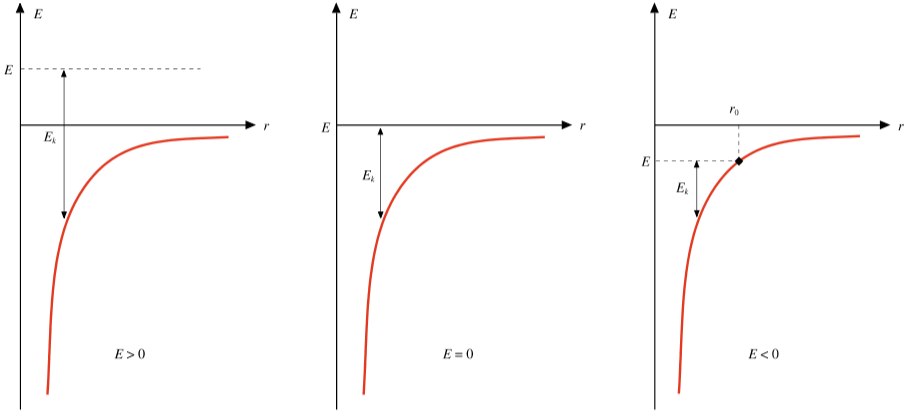
\includegraphics[width=0.9\linewidth]{Immagini/energia orbite.png}
    \caption{confronto tra energia meccanica, potenziale e cinetica per le diverse orbite.}
    \label{fig: energie orbite}
\end{figure}

L'energia totale di un sistema a due masse può assumere valore positivo, nullo o negativo a seconda che sia verificata una delle condizioni
\begin{equation}
    K>|U|,\quad K=|U|,\quad K<|U|.
\end{equation}
Nei grafici in figura \ref{fig: energie orbite} sono rappresentati i tre casi: $r$ è la distanza mutua, $E$ è l'energia totale costante, la doppia freccia indica la differenza $E-U=K$ per un particolare valore di $r$, mentre la curva continua mostra $U=-\gamma m_1m_2/r$ ed è la stessa nei tre casi. Nei primi due casi non ci sono limiti, mentre nel terzo $r$ è limitato da $r\le r_0$, altrimenti si avrebbe $K>E$. Queste considerazioni vengono parzialmente corrette a seguito del calcolo esplicito per l'energia totale del sistema di due masse, valida anche per orbite non circolari. In particolare, si otterrà che se $E>0$ l'orbita è iperbolica, se $E=0$ l'orbita è parabolica, mentre se $E<0$ l'orbita è ellittica. Le traiettorie ellittiche possono essere di tre diverse, di cui una in realtà circolare. 

\section{Teorema di Gauss per \texorpdfstring{$\vG$}{G} e distribuzioni sferiche}
Si consideri un certo numero di masse e una superficie geometrica chiusa che ne racchiude $n$. In ogni punto della superficie si determina $\vG$, che è dovuto a tutte le masse presenti, sia interne che esterne, e si calcola la quantità scalare
\begin{equation}
    d\Phi=\vG\cdot\hatu_N\,dS,
\end{equation}
dove $\hatu_N$ è il vettore normale alla superficie, che si assume essere orientato verso l'esterno, e $dS$ è l'elemento di superficie intorno al quale è calcolato $\vG$. L'integrale esteso a tutta la superficie restituisce 
\begin{equation}
    \Phi=\oint d\Phi=\oint\vG\cdot\hatu_N\,dS,
\end{equation}
che prende il nome di flusso del campo gravitazionale attraverso la superficie $S$. A questo punto è fondamentale il seguente teorema.
\begin{teo}[teorema di Gauss]
    Il flusso del campo gravitazionale attraverso una superficie chiusa è proporzionale alla somma delle masse interne alla superficie secondo
    \begin{equation}
        \Phi=-4\pi\gamma\sum_{i=1}^nm_i.
    \end{equation}
\end{teo}
\begin{proof}
    Il differenziale del flusso di campo gravitazionale è
    \begin{equation}
        d\Phi=\vG\cdot\hatu_N\,dS=-\gamma\frac{m}{r^2}(\hatu_r\cdot\hatu_N)\,dS=-\gamma\frac{m}{r^2}\,dS,
    \end{equation}
    dove il differenziale $dS$ corrisponde ad una porzione infinitesima di superficie sferica che, in coordinate sferiche, è data da
    \begin{equation}
        dS=r^2\sin{\theta}\,d\theta d\phi.
    \end{equation}
    Quindi integrando il differenziale $d\Phi$, in cui si è sostituito $dS$, si ottiene
    \begin{equation}
        \Phi=\int d\Phi=-\gamma\frac{m}{r^2}r^2\int_0^{\pi}\sin{\theta}\,d\theta\int_0^{2\pi}d\phi=-4\pi\gamma m.
    \end{equation}
    La dimostrazione è analoga nel caso in cui il campo gravitazione sia $\vG=\nsum_i\vG_i$ e la massa compresa all'interno della superficie di Gauss sia $m=\nsum_im_i$. 
\end{proof}
Il teorema permette di verificare che il campo generato da una distribuzione sferica di massa è uguale a quello generato da una massa puntiforme identica posta nel centro della distribuzione. Si consideri quindi una distribuzione sferica superficiale uniforme di massa $m$ di raggio $R$. Nel punto $P$, esterno alla distribuzione, il campo $\vG$ è radiale ed è dovuto alla somma di contributi simmetrici, se così non fosse la distribuzione non sarebbe uniforme. In qualsiasi altro punto che abbia la stessa distanza $r$ di $P$ dal centro della distribuzione il campo ha lo stesso valore, in quanto dipende solo dal modulo di $r$, ossia è radiale $\vG=G(r)\hatu_r$. Per calcolare $G(r)$ si considera come superficie di integrazione una seconda superficie sferica $S$ concentrica alla distribuzione di raggio $r\ge R$. In tal caso, si ha che il flusso attraverso $S$ è
\begin{equation}
    \Phi=\oint-G(r)\hatu_r\cdot\hatu_N\,dS=G(r)\oint dS=4\pi r^2G(r).
\end{equation}
Dato che per il teorema di Gauss $\Phi=4\pi\gamma m$, uguagliando le due espressione del flusso si ottiene
\begin{equation}
    G(r)=\gamma\frac{m}{r^2},
\end{equation}
come se $m$ fosse concentrata nel centro della distribuzione di massa. Il risultato vale per $r\ge R$, invece all'interno, per $r<R$, qualsiasi superficie di integrazione si consideri non contiene alcuna massa e quindi il flusso attraverso essa è nullo, in altre parole $G=0$ per $r<R$.

Se $m$ è distribuita uniformemente in tutto il volume sferico, all'esterno l'espressione di $G(r)$ è la medesima, mentre per $r<R$ il valore non è più nullo. Sfruttando la simmetria radiale, all'interno di una superficie sferica $S_1$ di raggio $r\le R$ la massa contenuta $m(r)$ è minore di $m$. Dato che la distribuzione è uniforme, il rapporto tra $m(r)$ e $m$ è uguale al rapporto tra i volumi occupati, ovvero a $r^3/R^3$, per cui
\begin{equation}
    m(r)=\frac{mr^3}{R^3}.
\end{equation}
Sostituendo questa nell'espressione di $\Phi$ e usando il teorema di Gauss si ha
\begin{equation}
    \Phi(r)=4\pi r^2G(r)=4\pi\gamma m(r)=4\pi\gamma m\frac{r^3}{R^3},
\end{equation}
da cui
\begin{equation}
    G(r)=\gamma\frac{m}{R^3}r.
\end{equation}
Riassumendo, l'intensità del campo gravitazionale in funzione della distanza $r$ dal centro della distribuzione volumica sferica omogenea di massa $m$ è
\begin{equation}
\label{eq: campo gravitazionale in funzione di r}
    G(r)=\begin{cases}
        \gamma\dfrac{m}{r^2},\quad r\ge R\\[1.5ex]
        \gamma\dfrac{m}{R^3}r,\quad r<R
    \end{cases}.
\end{equation}
\begin{obs}
    Considerando una massa puntiforme $m_p$, da \eqref{eq: campo gravitazionale in funzione di r} si ha che la forza subita da $m_p$ è
    \begin{equation}
        \vF=m_p\vG=-\gamma\frac{m_pm}{R^3}r\hatu_r=-K\vr,
    \end{equation}
    ossia è una forza di tipo elastico. Se lungo un diametro della distribuzione si creasse un foro e si lasciasse cadere la massa $m_p$ all'interno di esso, questa si muoverebbe di moto armonico con ampiezza pari al raggio $R$ della distribuzione. 
\end{obs}
Dato che l'espressione di $G(r)$ per distanze maggiori del raggio della distribuzione sferica è sempre la stessa, si può dimostrare che la forza gravitazionale tra due sfere omogenee di masse $m_1$ e $m_2$, poste ad una distanza $r$ tra i loro centri $O_1$ e $O_2$, è uguale alla forza gravitazionale tra due masse puntiformi $m_1$ e $m_2$ distanti $r$.

Ciascun elemento $dm_2$ della seconda sfera è soggetto ad una forza gravitazionale equivalente a quella generata da una massa puntiforme $m_1$ posta in $O_1$. Quindi, dalla definizione di $\vG$ e di forza di attrazione gravitazionale si ha
\begin{equation}
    d\vF_{1,2}=dm_2\vG_1=-\gamma\frac{m_1 dm_2}{r_1^2}\hatu_1.
\end{equation}
Per calcolare la risultante di tutte queste forze $d\vF_{1,2}$ si osserva che, il base al terzo principio di Newton, $dm_2$ esercita in $O_1$ una forza uguale e opposta
\begin{equation}
    d\vF_{2,1}=-d\vF_{1,2}=\gamma\frac{m_1 dm_2}{r_1^2}\hatu_1,
\end{equation}
e che l'effetto risultante in $O_1$ è quello di una massa puntiforme $m_2$ posta in $O_2$. Quindi, la forza risultante, in modulo, è
\begin{equation}
    F=\gamma\frac{m_1m_2}{r^2}.
\end{equation}
Il risultato è vero anche se i raggi delle due sfere sono confrontabili con la distanza tra i due centri o anche se le sfere sono a contatto. Si può anche lasciare l'ipotesi che la distribuzione delle masse sia omogenea, in quanto è sufficiente che tale distribuzione vari unicamente in funzione della distanza dal centro in modo da conservare la simmetrica sferica.
\begin{obs}
    Queste proprietà sono tutte derivate dal teorema di Gauss e quindi valgono per tutti i campi proporzionali a $1/r^2$, compreso il campo elettrostatico. 
\end{obs}

\subsection{Energia gravitazionale di una sfera omogenea}
Si supponga di costruire una sfera di massa $m$ e raggio $R$ per gusci successivi, ognuno compreso tra $r$ e $r+dr$. Il lavoro per portare da distanza infinita a distanza $r$ dal centro la massa $dm$ che si distribuisce nel guscio tra $r$ ed $r+dr$ è
\begin{equation}
    dW=-dU=\gamma\frac{m(r)dm}{r}.
\end{equation}
Sapendo che $m(r)=mr^3/R^3$, si ha
\begin{equation}
    dm=\frac{m}{R^3}d(r^3)=\frac{3mr^2}{R^3}dr.
\end{equation}
Pertanto
\begin{equation}
    dW=3\gamma\frac{m^2}{R^6}r^4\,dr,
\end{equation}
la quale integrata tra $0$ ed $R$ restituisce il lavoro necessario per costruire l'intera sfera
\begin{equation}
    W=\frac{3}{5}\gamma\frac{m^2}{R}.
\end{equation}
Il lavoro è fornito dalla forza gravitazionale ed è uguale a $U_i-U_f$. Però, $U_i=0$ in quanto inizialmente tutte le parti della sfera sono infinitamente lontane tra di loro, quindi
\begin{equation}
    U_f=-W=-\frac{3}{5}\gamma\frac{m^2}{R}.
\end{equation}

\subsection{Velocità di fuga e orbita circolare}
La velocità di fuga è la velocità minima necessaria affinché un oggetto possa sfuggire all'attrazione gravitazionale di un corpo celeste senza ulteriore apporto di energia. Si parte dall'uguaglianza tra l'energia cinetica iniziale dell'oggetto e l'energia potenziale gravitazionale necessaria per allontanarlo indefinitamente. L'energia cinetica di $m$ è data dall'espressione $mv^2/2$, mentre l'energia potenziale gravitazionale in prossimità della superficie del pianeta di massa $M$ è $-\gamma m M/R_T$. Affinché l'oggetto possa allontanarsi indefinitamente, la sua energia meccanica totale deve essere nulla, ovvero
\begin{equation}
    \frac{1}{2}mv^2-\gamma\frac{mM}{R_T} = 0.
\end{equation}
Risolvendo rispetto a $v$, si ottiene l'espressione della velocità di fuga:
\begin{equation}
    v = \sqrt{\frac{2 \gamma M}{R_T}}.
\end{equation}
Un altro aspetto importante riguarda l'energia potenziale di un oggetto in orbita a una distanza $R_T+h$ dal centro del pianeta. In questo caso, l'energia potenziale gravitazionale è data da
\begin{equation}
    U(R_T + h) = -\gamma\frac{mM}{R_T + h}.
\end{equation}
Nel caso in cui $h\ll R_T$, si può espandere l'espressione tramite l'approssimazione
\begin{equation}
    \frac{1}{R_T + h} \approx \frac{1}{R_T} \left( 1 - \frac{h}{R_T} \right).
\end{equation}
Pertanto, l'energia potenziale può essere riscritta come
\begin{equation}
    U(R_T + h) \approx -\frac{\gamma m M}{R_T} + \frac{\gamma m M}{R_T^2} h.
\end{equation}
Ricordando che $g=\gamma M/R_T^2$ e notando che il termine $-\gamma m M/R_T$ è una costante, l'energia potenziale $U$ si può scrivere come
\begin{equation}
    U(R_T+h)=mgh+costante.
\end{equation}
Quindi, ridefinendo in modo opportuno la costante è possibile scrivere l'energia potenziale gravitazionale $U$ rispetto alla superficie terrestre come $mgh$. 

\section{Moto dei pianeti}
L'obiettivo è ora dimostrare che le orbite dei pianeti sono ellittiche e che il quadrato del periodo di rivoluzione è proporzionale al cubo del semiasse maggiore, ossia si vogliono dimostrare la prima e la terza legge di Keplero. 

Si considerino due masse isolate $m$ ed $M$, che possono essere indifferentemente puntiformi o estese, tra le quali agisca una forza gravitazionale $\vF=\gamma mM/r^2$. In un sistema di riferimento inerziale 
\begin{equation}
    \vF=m\va_m,\quad\vF=M\va_M.
\end{equation}
L'accelerazione relativa di $m$ rispetto ad $M$ è
\begin{equation}
    \va=\va_m-\va_M=\bigg(\frac{1}{m}+\frac{1}{M}\bigg)\vF=\frac{\vF}{\mu},
\end{equation}
dove $\mu=mM/(m+M)$ è detta massa ridotta del sistema. Pertanto, $\vF=\mu\va$. Quindi, il moto relativo di due punti materiali sottoposti alla loro interazione mutua è equivalente al moto di un punto con massa uguale alla massa ridotta e sottoposto ad una forza uguale a quella di interazione mutua. In altre parole, l'equazione del moto di $m$ rispetto ad $M$, $\vF=\mu\va$, è identica a quella valida in un sistema di riferimento inerziale in cui $M$ è fissa, con il solo scambio $m\to\mu$ e con la forza $\vF$ immutata, anche se $M$ si muove di moto accelerato. Il risultato non dipende dal tipo di forza agente e mostra che il problema del moto relativo di due punti materiali può sempre essere ricondotto a quello di un unico punto. In questo caso, l'equazione del moto è
\begin{equation}
\label{eq: eqzn. moto dei pianeti}
    -\gamma\frac{mM}{r^2}\hatu_r=\mu a_r\hatu_r,
\end{equation}
dove $a_r$ è il modulo dell'accelerazione radiale.

Dato che si sta studiando un sistema isolato di due punti che interagiscono tra di loro tramite la forza di attrazione gravitazionale, che è una forza conservativa, allora valgono la conservazione della quantità di moto totale $\vp$, che implica la velocità del centro di massa $\vcm$ costante, la conservazione del momento angolare $\vL$ e la conservazione dell'energia meccanica $E$. Il fatto che $\vL=\vr\times\vp$ è costante, implica che il moto si svolge sul piano identificato dai vettori $\vr$ e $\vp$. Per descrivere il moto si usano le coordinate polari, in tal caso la velocità ha la forma
\begin{equation}
    \vv=\frac{dr}{dt}\hatu_r+r\frac{d\theta}{dt}\hatu_\theta.
\end{equation}
L'energia meccanica è data da
\begin{equation}
    \begin{split}
        E&=\frac{1}{2}\mu(\vv\cdot\vv)-\gamma\frac{mM}{r} \\
        &=\frac{1}{2}\mu\bigg(\frac{dr}{dt}\bigg)^2+\frac{1}{2}\mu r^2\bigg(\frac{d\theta}{dt}\bigg)^2-\gamma\frac{mM}{r} \\
        &=\frac{1}{2}\mu\bigg(\frac{dr}{dt}\bigg)^2+\frac{1}{2}\mu\frac{L^2}{r^2\mu^2}-\gamma\frac{mM}{r} \\
        &=\frac{1}{2}\mu\bigg(\frac{dr}{dt}\bigg)^2+\frac{L^2}{2\mu r^2}-\gamma\frac{mM}{r},
    \end{split}
\end{equation}
dove si è usata la relazione
\begin{equation}
    L=\mu r^2\frac{d\theta}{dt}\Rightarrow\frac{L}{\mu}=r^2\frac{d\theta}{dt}.
\end{equation}
Dato che gli ultimi due addendi dipendono solo da $r$, si introduce il potenziale efficace
\begin{equation}
    U_{eff}(r)=\frac{L^2}{2\mu r^2}-\gamma\frac{mM}{r}.
\end{equation}
Quindi, l'energia meccanica è
\begin{equation}
    E=\frac{1}{2}\mu\bigg(\frac{dr}{dt}\bigg)^2+U_{eff}(r).
\end{equation}
Osservando la forma del potenziale efficace, si nota che per piccoli valori di $r$ il termine dominante è il primo, proporzionale ad $1/r^2$, mentre per grandi valori di $r$ il termine dominante è il secondo, proporzionale ad $1/r$. Il grafico del potenziale efficace in funzione di $r$ è mostrato nella figura \ref{fig: potenziale efficace}.
\begin{figure}[h]
    \centering
    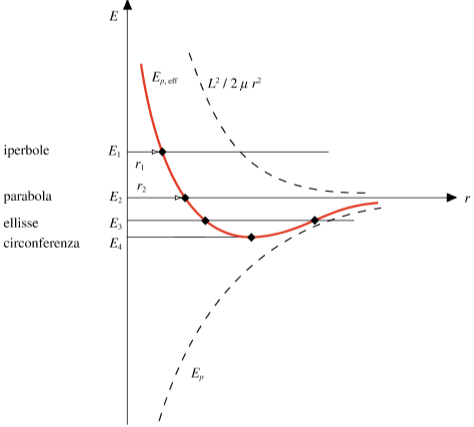
\includegraphics[width=0.6\linewidth]{Immagini/potenziale efficace.png}
    \caption{andamento del potenziale efficace in funzione della distanza tra $m$ ed $M$.}
    \label{fig: potenziale efficace}
\end{figure}


\paragraph{Proprietà delle coniche.} Prima di studiare ulteriormente il moto dei pianeti, è necessario introdurre alcune proprietà delle coniche. Prima di tutto, una conica è definita come il luogo dei punti per i quali il rapporto tra la distanza da un punto, detto fuoco, e la distanza da una retta, detta direttrice, è pari ad una costante positiva $\epsilon$ che prende il nome di eccentricità ed è data da
\begin{equation}
\label{eq: defn. eccentricità}
    \epsilon=\frac{\overline{PF}}{\overline{PQ}}=\frac{r}{r+d\cos\theta},
\end{equation}
dove $d$ è la distanza tra il fuoco e la direttrice, un parametro noto. In coordinate polari, partendo da \eqref{eq: defn. eccentricità}, l'equazione delle conica di centro $F$ è
\begin{equation}
\label{eq: eqzn. coniche}
    \frac{1}{r}=\frac{1}{\epsilon d}-\frac{\cos\theta}{d}.
\end{equation}
La conica può essere un'ellisse se $\epsilon<1$, una parabola se $\epsilon=1$, un'iperbole se $\epsilon>1$, oppure degenera in una circonferenza se $\epsilon=0$. In particolare, per un'ellisse di semiassi $a$ e $b$ valgono le relazioni
\begin{equation}
\label{eq: relazioni ellisse}
    a=\frac{\epsilon d}{1-\epsilon^2},\quad b=a\sqrt{1-\epsilon^2},\quad\epsilon^2=1-\frac{b^2}{a^2},\quad A=\pi a^2\sqrt{1-\epsilon^2}.
\end{equation}

Per esprimere l'accelerazione radiale $\va_r$ in \eqref{eq: eqzn. moto dei pianeti} si può usare la formula di Binet
\begin{equation}
    \va_r=-\frac{L^2}{\mu^2r^2}\bigg[\frac{d^2}{d\theta^2}\bigg(\frac{1}{r}\bigg)+\frac{1}{r}\bigg]\hatu_r.
\end{equation}
Sostituendola in \eqref{eq: eqzn. moto dei pianeti} e considerando i moduli si ottiene
\begin{equation}
    -\gamma\frac{mM}{r^2}=-\mu\frac{L^2}{\mu^2r^2}\bigg[\frac{d^2}{d\theta^2}\bigg(\frac{1}{r}\bigg)+\frac{1}{r}\bigg],
\end{equation}
da cui si trova l'equazione differenziale
\begin{equation}
    \frac{d^2}{d\theta^2}\bigg(\frac{1}{r}\bigg)+\frac{1}{r}=\gamma\mu\frac{mM}{L^2},
\end{equation}
la cui soluzione è la funzione $r(\theta)$ che corrisponde alla traiettoria di $m$ rispetto ad $M$ in coordinate polari. A primo membro si può riconoscere la struttura dell'equazione del moto armonico semplice con un termine aggiuntivo che la rende non omogenea. La soluzione generale di questa equazione è $A\cos\theta+S_p$, dove $S_p$ è una soluzione particolare dell'equazione di partenza. Una soluzione particolare è uguale al termine che compare a secondo membro, ossia $S_p=\gamma\mu mM/L^2$. Pertanto, la soluzione dell'equazione differenziale è
\begin{equation}
\label{eq: soluzione eq. diff.}
    \frac{1}{r}=\gamma\mu \frac{mM}{L^2}+A\cos{\theta},  
\end{equation}
che ha la stessa forma dell'equazione delle coniche \eqref{eq: eqzn. coniche}. Pertanto, la traiettoria è una conica. Dal confronto di \eqref{eq: soluzione eq. diff.} con \eqref{eq: eqzn. coniche} si ottiene che
\begin{equation}
    L^2=\gamma\mu mM\epsilon d.
\end{equation}
Quindi, i parametri della traiettoria $\epsilon$ e $d$ stabiliscono il valore costante del momento angolare della massa $m$. 

L'energia meccanica di $m$ è la somma dell'energia cinetica e dell'energia potenziale
\begin{equation}
    E=\frac{1}{2}\mu\bigg(\frac{dr}{dt}\bigg)^2+\frac{1}{2}\mu r^2\bigg(\frac{d\theta}{dt}\bigg)^2-\gamma\frac{mM}{r}. 
\end{equation}
I termini che compaiono a secondo membro di questa equazione possono essere riscritti come segue. Per il primo membro si riprende l'equazione \eqref{eq: eqzn. coniche} e ne si prende la derivata, ottenendo
\begin{equation}
    \frac{d}{dt}\bigg(\frac{1}{r}\bigg)=\frac{d}{dt}\bigg(\frac{1}{\epsilon d}-\frac{\cos\theta}{d}\bigg)\Rightarrow\frac{dr}{dt}=-\frac{r^2\sin\theta}{d}\frac{d\theta}{dt}.
\end{equation}
Per il secondo termine, dato che la forza gravitazionale è una forza centrale si può usare 
\begin{equation}
    L=\mu r^2\frac{d\theta}{dt},
\end{equation}
in modo da poter scrivere che
\begin{equation}
    \frac{1}{2}\mu r^2\bigg(\frac{d\theta}{dt}\bigg)^2=\frac{1}{2}\frac{L^2}{\mu r^2}.
\end{equation}
Infine, per il terzo termine usando che $L^2=\gamma\mu mM\epsilon d$ si ha che
\begin{equation}
    -\gamma\frac{mM}{r}=-\frac{L^2}{\epsilon d\mu r}.
\end{equation}
Mettendo insieme questi risultati si ha che l'energia meccanica è
\begin{equation}
    E=\frac{1}{2}\frac{\sin^2\theta}{d^2}\frac{L^2}{\mu}+\frac{1}{2}\frac{L^2}{\mu r^2}-\frac{L^2}{\epsilon d\mu r}.
\end{equation}
Utilizzando l'equazione \eqref{eq: eqzn. coniche} per riscrivere $1/r$ ed $1/r^2$, insieme alla relazione $L^2=\gamma\mu mM\epsilon d$, si ottiene l'espressione finale dell'energia meccanica
\begin{equation}
\label{eq: energia meccanica corpi celesti}
    E=\frac{L^2}{2\mu\epsilon^2 d^2}(\epsilon^2-1)=\gamma\frac{mM}{2\epsilon d}(\epsilon^2-1).
\end{equation}
Dunque, anche l'energia meccanica, costante perché la forza agente è conservativa, è determinata dai parametri dell'orbita. Viceversa, fissati i valori di $L$ ed $E$ si possono ricavare $\epsilon$ e $d$. 
\begin{obs}
    L'equazione \eqref{eq: energia meccanica corpi celesti} conferma il fatto che quando $\epsilon<1$ l'orbita è ellittica e l'energia è negativa, quando $\epsilon>1$ l'orbita è iperbolica e l'energia è positiva, mentre quando $\epsilon=1$ l'orbita è parabolica e l'energia è nulla.
\end{obs}
Nel caso particolare delle orbite ellittiche, usando le relazioni \eqref{eq: relazioni ellisse}, si hanno
\begin{equation}
\label{eq: energia meccanica e mom. angolare per orbite ellittiche}
    E=-\gamma\frac{mM}{2a},\quad L^2=\gamma\mu mMa(1-\epsilon^2).
\end{equation}
Data l'energia meccanica $E$, è fissato solo il semiasse maggiore ma non l'eccentricità $\epsilon$. Dunque, a parità di energia si possono avere ellissi diverse (stesso $a$, ma diversa $\epsilon$) con momento angolare diverso, a conferma che $E$ ed $L$ sono indipendenti. Infine, per una forza centrale, la velocità areale è
\begin{equation}
    \frac{dA}{dt}=\frac{L}{2\mu}=\frac{A}{T},
\end{equation}
dove $T$ è il periodo di rivoluzione. Risolvendo per $L$ e usando la relazione per l'area di un ellisse vista in \eqref{eq: relazioni ellisse}, si ha
\begin{equation}
    L=2\mu\frac{A}{T}=2\mu\frac{\pi a^2}{T}\sqrt{1-\epsilon^2}.
\end{equation}
Confrontando quest'ultima con la seconda di \eqref{eq: energia meccanica e mom. angolare per orbite ellittiche} si ha
\begin{equation}
    \frac{4\pi^2\mu^2a^4(1-\epsilon^2)}{T^2}=\gamma\mu mMa(1-\epsilon^2),
\end{equation}
da cui si ricava la terza legge di Keplero
\begin{equation}
    T^2=\frac{4\pi^2\mu a^3}{\gamma mM}=\frac{4\pi^2}{\gamma(m+M)}a^3=Ka^3.
\end{equation}
\begin{obs}
    La costante $K$ presente nella terza legge di Keplero è praticamente uguale per tutti i pianeti. Infatti, se $m\ll M$, allora
    \begin{equation}
        K=\frac{4\pi^2}{\gamma(m+M)}\approx\frac{4\pi^2}{\gamma M}.
    \end{equation}
\end{obs}

\end{document}
